% !TeX program = xelatex
% 编译：latexmk -xelatex -interaction=nonstopmode -halt-on-error main.tex
\documentclass[UTF8,a4paper,12pt,oneside,openany,fontset=none]{ctexrep}
\usepackage[margin=2.5cm,headheight=16pt]{geometry}
\setmainfont{texgyretermes-regular.otf}[
  BoldFont=texgyretermes-bold.otf,ItalicFont=texgyretermes-italic.otf,
  BoldItalicFont=texgyretermes-bolditalic.otf]
\setsansfont{texgyreheros-regular.otf}[
  BoldFont=texgyreheros-bold.otf,ItalicFont=texgyreheros-italic.otf,
  BoldItalicFont=texgyreheros-bolditalic.otf]
\setmonofont{lmmono10-regular.otf}[Scale=MatchLowercase]
\setCJKmainfont{Noto Serif CJK SC}
\setCJKsansfont{Noto Sans CJK SC}
\setCJKmonofont{Noto Sans Mono CJK SC}
\usepackage{amsmath,amssymb,booktabs,array,tabularx,longtable}
\usepackage{graphicx,xcolor,enumitem,fancyhdr}
\usepackage{tikz}
\usetikzlibrary{arrows.meta,positioning,fit,calc}
\usepackage{xurl}
\usepackage[unicode,hidelinks,bookmarksnumbered,hypertexnames=false]{hyperref}
\hypersetup{pdftitle={基于紫光同创 FPGA 的任意角度畸变矫正系统设计报告},
  pdfauthor={参赛团队}}
\definecolor{TemplateBlue}{RGB}{22,75,114}
\definecolor{TemplateGray}{RGB}{245,247,249}
\newcommand{\sourcefile}[1]{\par\noindent{\footnotesize\textcolor{gray}{工程依据：}#1}\par}
\newcolumntype{Y}{>{\raggedright\arraybackslash}X}
\renewcommand{\arraystretch}{1.25}
\setlength{\parindent}{2em}
\setlength{\emergencystretch}{2em}
\setlist{nosep,leftmargin=2em}
\setcounter{tocdepth}{2}
\ctexset{chapter={format=\centering\Large\bfseries},section={format=\large\bfseries}}
\pagestyle{fancy}
\fancyhf{}
\fancyhead[L]{\small 任意角度畸变矫正系统设计报告}
\fancyhead[R]{\small 项目设计报告}
\fancyfoot[C]{\thepage}
\begin{document}
\begin{titlepage}
  \centering
  \vspace*{1cm}
  {\Large 全国大学生嵌入式芯片与系统设计竞赛\par}
  \vspace{0.5cm}
  {\large 2026 FPGA 赛道\quad 紫光同创选题二\par}
  \vspace{2cm}
  {\Huge\bfseries 基于紫光同创 FPGA 的\par 任意角度畸变矫正系统\par}
  \vspace{0.7cm}
  {\LARGE 项目设计报告\par}
  \vspace{1.4cm}
  \begin{tabular}{rl}
    作品名称： & 基于 FPGA 的图像畸变与姿态矫正系统 \\
    报告类别： & 项目设计与验证报告 \\
    报告日期： & 2026 年 10 月 25 日
  \end{tabular}
  \vfill
  {\small 实现平台：PGL50H FPGA / MES50HP 开发板\par}
  {\small 系统设计、算法部署与验证结果\par}
\end{titlepage}
\pagenumbering{Roman}
\chapter*{模板使用说明}
\addcontentsline{toc}{chapter}{模板使用说明}
本模板根据本目录的 \path{problem.md} 及相邻 \path{../Pgl50h/} 工程整理，
适用于“基于紫光同创 FPGA 的任意角度的畸变矫正”选题。
模板以 2026 年 10 月 22 日 CP2102 位流及其归档证据为主要基线，
预填系统架构、算法、模块职责和已有验证数据。所有蓝色“待补充”字段、撰写提示和图片框，
均应在正式提交前完成替换或删除。

本文使用三种结果口径：\textbf{工程实现}描述源码中已有的功能；
\textbf{仿真/实现工具结果}引用已有 RTL 日志及 PDS 报告；
\textbf{实板测量}留待实际硬件验证。当前归档身份文件明确标记
\path{board_programmed=false}、\path{board_tested=false}。
模板整理过程中仅查阅工程与验证记录，未重新运行 FPGA 综合、布局布线或 RTL 回归。

报告中的“任意角度”沿用赛题名称；当前基线仅使用 yaw/pitch，默认每轴约
$\pm15^\circ$，roll 不参与变换。默认实时分块路径使用最近邻采样；
历史串行路径保留双线性，但其性能不适用本模板中的分块吞吐数据。
1080p60 表示输入/输出扫描时序，1080p30 表示当前行为模型仿真的新矫正帧更新能力。

\guide{首先填写封面和第 1 章指标，再补充第 6、7 章实测数据。
如更换源码、标定或位流，应同时更新基线、结果表和附录证据，不能沿用旧性能结论。}

\chapter*{摘要}
\addcontentsline{toc}{chapter}{摘要}
针对镜头畸变和相机姿态变化引起的图像几何失真，本文基于紫光同创
PGL50H-FBG484-6 FPGA，设计面向 $1920\times1080$ 视频的几何矫正系统。
系统通过 MS7200 接收 HDMI RGB888 数据，在量化为 RGB565 前完成帧自适应
Gamma 预处理，并将源帧写入 DDR3。矫正器根据相机标定内参、二阶径向畸变系数及
逐帧锁存的 IMU yaw/pitch，通过定点逆投影生成采样坐标，采用
$128\times32$ 双槽分块缓存和突发访问生成结果帧，经 MS7210 输出 HDMI 视频。
板载 CP2102 提供去畸变、姿态补偿和 Gamma 的独立控制及亮度统计遥测。

当前基线在包含并发采集、渲染、显示及 DDR 停顿的完整 RTL 行为模型中，
达到约 30.000030 个新结果帧/秒，最慢观测渲染时间为 33.14614 ms；
显示扫描为 60 Hz。PDS 2025.2 最终双工作角时序检查通过，
最终占用 104/134 个 DRM 位置、16,878/42,800 个 LUT（含常量和旁路）。
上述数据来自归档仿真及实现报告；实板端到端延迟、真实帧率、直线度及
MTF50/SFR 等结果为\fillin{实测结果及最终结论}。

\noindent\textbf{关键词：}紫光同创 FPGA；畸变矫正；逆投影；IMU；分块缓存；自适应 Gamma

\guide{正式摘要建议保留“问题—方法—结果—结论”结构。
补齐实测后更新结果段，并保持与第 7 章一致；不能把渲染耗时写成端到端延迟。}

\tableofcontents
\clearpage
\pagenumbering{arabic}
\chapter{赛题需求分析}
\label{chap:introduction}

\section{研究背景与应用价值}
本项目面向 2026 年全国大学生嵌入式芯片与系统设计竞赛 FPGA 创新设计赛道，
选择紫光同创选题二“基于紫光同创 FPGA 的任意角度的畸变矫正”。
该赛题要求利用国产 FPGA 平台构建完整的视频处理系统，在真实相机标定参数的基础上，
实现图像几何矫正，并进一步结合姿态感知、硬件流水线及自适应增强，
提升动态场景下的实时处理能力与成像效果\cite{problem}。

在机器视觉、自动驾驶、智能交通和视觉测量等应用中，图像不仅用于观察，
也是目标定位与空间测量的数据来源。镜头的径向畸变可能使直线呈现桶形或枕形弯曲，
切向畸变则会造成局部位置偏移；相机倾斜和转动还会改变目标的投影关系。
这些因素会影响图像拼接、目标检测及尺寸测量的准确性。
因此，需要将镜头畸变补偿与相机姿态变换结合起来，使输出图像保持符合预期的几何关系。

高分辨率视频的几何矫正需要逐像素进行坐标变换与重采样，
且变换后的源像素访问通常不连续。FPGA 可将坐标计算、图像缓存和视频接口组织为
并行模块与流水线，为持续视频处理提供可控的时序基础。
其实现难点在于有限逻辑、乘法和片内存储资源下，协调运算精度、外部存储带宽与处理延迟。
本项目以可改变姿态的相机为应用对象，通过云台调整拍摄方向、IMU 提供姿态信息，
在 FPGA 上完成图像矫正与增强，并由上位机观察输出和控制功能，
形成可用于动态演示与客观测评的实验系统。

\section{赛题任务分解}
依据选题指南正文第 10--12 页，本系统的任务分为基础功能与高阶功能两部分。
基础功能构成从视频输入到矫正输出的数据链路，高阶功能进一步解决动态姿态、
实时吞吐和复杂光照条件下的适应性问题\cite{problem}。

\subsection{基础功能需求}
\begin{enumerate}[label=（\arabic*）]
  \item \textbf{图像采集、缓存与显示。}
  实现 HDMI 或摄像头接口的视频输入、图像缓存和显示输出，保证像素数据与同步信号一致。
  本系统采用 HDMI 输入输出和 DDR3 帧缓存，为几何变换提供可寻址的源图像。
  该链路还需协调输入、存储和输出时钟域，避免读写冲突及画面撕裂。

  \item \textbf{畸变模型与坐标映射。}
  在 FPGA 中实现二阶径向及切向畸变模型，依据焦距、主点和畸变系数计算像素对应关系。
  标定参数应来源于真实相机，并保持标定分辨率、像素坐标约定与硬件实现一致。
  本系统采用输出像素驱动的逆映射，由理想输出位置反求畸变源图像中的采样坐标。

  \item \textbf{图像重采样与完整性。}
  根据映射得到的非整数坐标进行重采样，赛题给出双线性插值作为基础算法示例，
  并要求消除矫正后的黑边或空洞现象。
  设计中需分别处理离散映射产生的漏采样与变换后超出源视场的区域：
  逆映射可避免前者，后者需通过有效视场选择、裁切等策略控制，并评价其对视场的影响。
\end{enumerate}

\subsection{高阶功能需求}
\begin{enumerate}[label=（\arabic*）]
  \item \textbf{任意角度与动态矫正。}
  结合 IMU 或上位机指令，在相机倾斜、旋转时动态更新几何变换。
  姿态坐标轴、角度符号和安装零点应与图像坐标系保持一致；
  同一帧处理期间应采用一致的姿态参数，避免参数切换引起局部错位。
  动态验证需覆盖连续角度变化及不同测试图卡，记录支持的角度范围与边界行为。

  \item \textbf{硬件加速与流水线优化。}
  针对坐标映射中的乘除法、定点运算和非连续访存设计硬件流水线，
  通过缓存复用和突发传输提高外部存储效率。
  系统吞吐应包含采集、运算、访存和结果发布全过程，
  并满足持续视频处理所需的帧率与时序约束。

  \item \textbf{自适应图像预处理。}
  面向强光、夜间等复杂光照，在矫正前或矫正过程中加入自适应 Gamma 校正
  或直方图均衡等增强算法。本系统选择帧自适应 Gamma 方案，
  根据亮度统计调整映射曲线，并通过增强开关对比暗部细节、高光表现及帧间稳定性。
\end{enumerate}

\section{设计目标与评价指标}
\subsection{系统规格与实时处理目标}
赛题以 1080P@30fps 或 60fps 为实时处理标准的示例，
同时要求测量端到端硬件延迟，并在满足性能的前提下降低资源占用。
结合所选 PGL50H 器件与帧缓存结构，本系统将输入输出配置为
$1920\times1080$、60 Hz 扫描，将完整矫正结果的更新速率设为不低于 30 fps 的工程目标。
按有效图像区域计算，30 fps 对应每秒处理 62.208 百万个输出像素，
每个结果帧的平均时间预算约为 33.33 ms。

显示扫描率与矫正更新率分别统计：前者反映输出接口的扫描时序，
后者统计单位时间内由不同源帧生成的完整结果帧数量。
重复显示上一结果帧不计入新的矫正帧，单帧渲染耗时也不等于端到端延迟。
端到端硬件延迟以 FPGA 视频输入侧接收某一可识别事件为起点、
视频输出侧输出其对应像素为终点；若使用相机和采集卡测量整条演示链路，
还需说明这些设备引入的额外延迟。

\subsection{算法精度与工程评价方法}
表~\ref{tab:requirements} 给出本系统依据赛题建立的评价项目。
赛题对清晰度、直线度和延迟给出了评价方向，但未规定统一的数值门限，
因此本报告采用固定图卡、固定测试区域和可重复的测量方法记录结果，
并结合软件参考与原始图像进行比较。

\begin{table}[htbp]\centering\small
\caption{系统设计目标与评价方法}\label{tab:requirements}
\begin{tabularx}{\textwidth}{>{\raggedright\arraybackslash}p{2.5cm}YY}
\toprule
评价项目 & 设计目标或评价重点 & 测量与判定方法 \\
\midrule
视频链路 & $1920\times1080$，60 Hz 输入输出扫描，RGB888 接口 & 检查有效像素数、同步时序、颜色和帧完整性 \\
标定与坐标精度 & 正确使用真实相机内参及畸变系数，控制定点误差 & 核对参数来源，与独立浮点参考比较最大及均方根坐标误差 \\
图像质量 & 直线无明显弯曲，边缘无明显拉伸或断裂 & 使用网格和斜边图卡，测量直线度及 MTF50 或 SFR，记录有效视场与无效区域比例 \\
实时性与延迟 & 完整矫正结果更新率 $\geq30$ fps，并降低链路延迟 & 按源帧身份统计发布率，分别测量渲染耗时和端到端延迟 \\
动态姿态 & 在声明的角度范围内连续更新，帧内参数一致 & 测试中间及边界角度、连续转动、零点和异常姿态输入 \\
自适应增强 & 改善复杂光照下的可见细节，控制亮度跳变 & 对比增强开关及亮暗切换场景，记录亮度统计和主客观效果 \\
资源与稳定性 & 资源占用不超过器件容量，满足时序并保持连续运行 & 检查 LUT、FF、APM、DRM 报告、CDC 处理及持续运行中的异常计数 \\
\bottomrule
\end{tabularx}
\end{table}

\section{开发约束与验证要求}
硬件平台采用赛题推荐的 MES50HP 开发板，核心处理器件为紫光同创 PGL50H，
使用 Verilog HDL 开发，采用 Pango Design Suite（PDS）完成综合、布局布线、
时序分析和位流生成。标定与测试环境由参赛者自行准备，
需包含真实相机、棋盘格或圆点标定板、标定软件及上位机图像质量分析工具。
赛题列举 OpenCV 标定工具箱用于生成基准参数，本工程使用实际相机的 MATLAB 标定记录，
后续比较应统一参数含义、坐标约定及畸变模型。

工程实现需重点处理视频输入、存储控制、姿态接收和显示输出之间的跨时钟域通信，
合理分配片内存储并约束外部接口时序。功能划分、接口定义、关键定点格式和时序约束
应在代码及文档中保持一致。验证采用算法参考、RTL 仿真、FPGA 实现分析与板级测试
相结合的方式，保存与源码、约束和位流版本对应的记录。
决赛演示应能够连续输入实时视频，并在改变相机物理角度或更换图卡时展示输出效果。

\section{本报告的工作内容}
本报告围绕“视频采集与缓存、姿态与镜头模型、逐像素逆映射、图像重采样及显示”
组织系统设计，重点说明定点运算流水线、分块访存和帧级参数管理之间的配合。
第~\ref{chap:system}~章介绍开发平台、硬件组成与总体数据通路；
第~\ref{chap:algorithm}~章介绍标定参数、姿态变换、畸变模型及重采样方法；
第~\ref{chap:hardware}~章说明 FPGA 模块划分、存储调度与跨时钟域设计；
第~\ref{chap:control}~章介绍姿态通信、上位机控制及自适应 Gamma；
第~\ref{chap:verification}~章给出验证方案和板级测试方法；
第~\ref{chap:performance}~章分析帧率、延迟、资源及图像质量，最后总结局限与改进方向。

当前工程基线采用最近邻重采样，yaw/pitch 每轴支持范围约为 $\pm15^\circ$，
roll 未参与变换，所用标定的切向系数为零，无效源区域输出黑色。
因此，双线性插值的实时实现、非零切向场景、完整姿态自由度及黑边处理仍需单独评估。
已有归档提供 RTL 仿真和布局布线证据，实板画质与端到端延迟尚需测量；
后续各章据此说明实现范围，并以相应测试记录判定赛题要求的满足情况\cite{project,current}。

\chapter{系统总体方案设计}
\label{chap:system}

\section{开发平台与器件选型}
本系统选用搭载紫光同创 Logos 系列 PGL50H FPGA 的 MES50HP（盘古 50）开发板，
采用紫光同创 PDS 软件完成逻辑设计与实现。平台选型主要考虑视频流处理的并行性、
定点坐标变换的运算需求，以及图像缓存和外部接口的扩展能力。

\subsection{FPGA 芯片及资源配置}
MES50HP 核心板采用的 FPGA 完整型号为 PGL50H-6IFBG484，
属于紫光同创 Logos 系列，采用 40 nm 工艺，速度等级为 $-6$，温度等级为工业级，
封装为 FBG484，共有 484 个引脚。实际 PDS 工程将器件系列、型号、封装和速度等级
分别配置为 Logos、PGL50H、FBG484 和 $-6$，实现记录中的器件标识为
PGL50H-FBG484-6，与板卡手册给出的型号在这些配置项上一致。
根据硬件手册第 2.2.1 节，芯片主要逻辑与存储资源如表~\ref{tab:fpga-resources} 所示\cite{board}。

\begin{table}[htbp]\centering\small
\caption{PGL50H FPGA 主要资源及其在本系统中的用途}
\label{tab:fpga-resources}
\begin{tabularx}{\textwidth}{>{\raggedright\arraybackslash}p{4cm}>{\raggedright\arraybackslash}p{3.5cm}Y}
\toprule
资源类型 & 器件资源总量 & 本系统中的主要用途 \\
\midrule
六输入查找表（LUT6） & 42\,800 个 & 图像预处理、坐标变换及控制逻辑 \\
触发器（FF） & 64\,200 个 & 流水线寄存、状态保持及跨时钟域同步 \\
片内存储块（DRM） & 134 个，每个 18 Kbit & 图像分块缓存、查找表及 FIFO \\
乘法运算单元（APM） & 84 个 & 定点投影变换中的乘法运算 \\
\bottomrule
\end{tabularx}
\end{table}

畸变矫正需要对输出像素逐点计算源图像坐标，并与视频采集、缓存读写和显示输出
协同运行。FPGA 可将上述功能组织为并行模块和多级流水线；其中，APM 为定点乘法
提供专用运算资源，DRM 用于构建局部图像缓存和数据缓冲，LUT 与触发器实现
采样控制、数据调度和接口时序。上述资源配置为本系统的分块逆映射方案提供了硬件基础，
具体资源占用与时序结果在实现验证章节中给出。

\subsection{MES50HP 开发板}
MES50HP 由核心板和扩展底板组成，两者通过高速板对板连接器连接。
核心板集成 FPGA、存储器、配置 Flash、电源及复位电路，构成 FPGA 最小运行系统；
扩展底板提供视频、通信及通用 I/O 接口，便于连接输入输出设备并开展系统联调\cite{board}。
这种结构兼顾了核心处理电路的集成与外围接口的扩展，适合本系统从算法验证到完整
视频链路搭建的开发过程。

核心板提供 50 MHz、27 MHz 单端时钟源及 125 MHz 差分时钟源，其中
50 MHz 用作 FPGA 系统参考时钟，125 MHz 用作 HSST 高速收发器参考时钟。
本工程使用板载 50 MHz 和 27 MHz 参考时钟，并通过 PLL 生成所需的内部工作时钟
和视频输出像素时钟。板卡已有的时钟、电源、复位和 JTAG 配置条件，
为逻辑下载与调试提供了基础。各外部设备的型号、接口电路及连接方式在下一节说明。

\subsection{PDS 开发工具与工程组织}
本系统使用紫光同创 Pango Design Suite（PDS）作为 FPGA 开发工具，
实现工具为 PDS 2025.2 build 211867。PDS 面向紫光同创 FPGA 提供从
HDL 设计输入、逻辑综合、器件映射、布局布线到静态时序分析及位流生成的实现流程，
并配合厂商 IP 完成时钟与存储接口等基础模块的集成。

实际主工程文件为 \path{EmbFPGA.pds}，顶层模块为 \path{hdmi_ddr3_top}。
工程以 Verilog HDL 描述图像处理与控制逻辑，RTL 源码集中在 \path{src/} 目录；
PLL、读写缓存及 DDR3 控制器等 IP 位于 \path{ipcore/} 目录，并通过
\path{.idf} 文件加入工程。引脚、电气属性和时序约束由
\path{src/constraints/hdmi_ddr3_top.fdc} 管理。
开发时依据板卡手册核对引脚及接口电平，在 PDS 中完成综合与布局布线后，
结合资源报告和时序报告检查实现结果，再生成用于板级验证的配置位流。
实现记录关联工具、目标器件、约束文件与配置位流，保证结果可追溯。
\sourcefile{\path{../Pgl50h/EmbFPGA.pds}；\path{../Pgl50h/bitstream/pc_control_20261022_identity.json}}

\section{系统硬件设计}
\subsection{开发板与外部连接}
系统以 MES50HP 开发板为图像处理核心，板载 HDMI 接收、发送与 DDR3 存储接口
构成视频数据通路，UART 接口接收姿态并连接上位机。
图~\ref{fig:mes50hp} 给出开发板及主要接口分布。

\begin{figure}[htbp]\centering
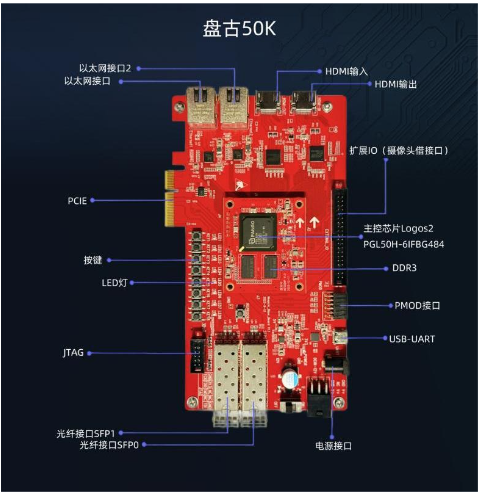
\includegraphics[width=0.66\textwidth]{chapter2/figures/tmp.png}
\caption{MES50HP 开发板及主要接口分布}
\label{fig:mes50hp}
\end{figure}

\subsection{相机与视频输入}
系统使用杰锐微通 USB 工业相机，视频输入规格为 $1920\times1080$、60 fps。
PC 通过 OpenCV 读取原始图像，由独立副屏 HDMI 输出至开发板 HDMI 输入接口；
板载 MS7200 将 HDMI 视频转换为 RGB888 并行像素数据。
该链路便于同时保存原始图像、向 FPGA 供图并开展同源对照分析。
PC 输出显示模式、采集格式和图像尺寸共同决定实际输入条件。

\subsection{视频输出与显示}
FPGA 输出的并行 RGB888 视频由板载 MS7210 编码为 HDMI，
经绿联 USB 采集卡送回 PC，与原始图像并排显示。
显示端独立维持 60 Hz 扫描，新矫正结果在安全帧边界交接。
采集卡与 PC 预览仅承担结果观测，不参与 FPGA 内部的帧率控制。

\subsection{IMU 与姿态输入}
姿态采集使用 RoboMaster C 型开发板，主控为 STM32F407，
传感器为 BMI088 六轴惯性测量单元。
STM32 经 SPI 获取三轴加速度与角速度，以 Mahony 算法解算 yaw、pitch、roll，
量化为有符号 16 bit 数据后，通过 UART 发送至 FPGA。
FPGA 将姿态与源帧关联，在同一帧矫正期间保持参数不变。
姿态采集、坐标约定和通信格式见附录~\ref{app:attitude-estimation}。

\subsection{双轴云台}
相机安装于自研二自由度云台，yaw、pitch 两轴由达妙电机驱动，
用于调整拍摄方向及构造静态、连续转动测试场景。
IMU 与相机保持刚性连接，使姿态输入对应相机的旋转状态。
云台机械轴、传感器轴与图像轴的对应关系决定姿态符号和矫正方向。

\subsection{上位机控制与状态监测}
PC 经板载 CP2102 USB 转串口接口连接 FPGA，
独立控制镜头去畸变、姿态矫正和自适应 Gamma，
并接收功能状态、曲线编号与帧亮度统计。
上位机同时提供双路视频预览、姿态模型显示和图卡质量分析，
软件结构与使用方法见附录~\ref{app:pc-host}。

\section{总体数据通路}
图~\ref{fig:architecture} 给出默认路径。RGB888 输入先完成帧自适应 Gamma，
再转换为 RGB565 以降低帧缓存带宽。采集、渲染和显示并行运行，矫正器使用
源帧对应的姿态和功能快照生成完整结果帧，显示端只在安全的帧边界交接结果。

\begin{figure}[htbp]\centering
\begin{tikzpicture}[
  block/.style={draw=TemplateBlue,rounded corners,fill=TemplateGray,
    align=center,minimum height=1.15cm,text width=4cm,font=\small},
  arrow/.style={-{Latex},thick,draw=TemplateBlue},node distance=0.55cm and 1.3cm]
\node[block] (in) {HDMI 输入 / MS7200\\RGB888};
\node[block,below=of in] (gamma) {帧自适应 Gamma\\RGB888 $\to$ RGB565};
\node[block,below=of gamma] (source) {DDR3 源帧槽 0 / 3\\帧姿态与功能快照};
\node[block,below=of source] (map) {逐像素定点逆投影\\$128\times32$ 双槽分块};
\node[block,right=of map] (sample) {源矩形缓存与采样\\结果块突发写回};
\node[block,right=of source] (result) {DDR3 结果帧槽 1 / 2\\VS 边界交接完整结果};
\node[block,right=of gamma] (out) {RGB565 $\to$ RGB888\\MS7210 / HDMI 60 Hz};
\node[block,right=of in] (ctrl) {IMU UART / CP2102\\姿态、控制与统计遥测};
\draw[arrow] (in)--(gamma);
\draw[arrow] (gamma)--(source);
\draw[arrow] (source)--(map);
\draw[arrow] (map)--(sample);
\node[text=TemplateBlue,inner sep=0pt] at ($(sample.north)!0.5!(result.south)$) {$\uparrow$};
\node[text=TemplateBlue,inner sep=0pt] at ($(result.north)!0.5!(out.south)$) {$\uparrow$};
\draw[arrow,dashed] (ctrl.west)--++(-0.35,0)|- (source.east);
\end{tikzpicture}
\caption{默认配置的系统数据与控制通路}\label{fig:architecture}
\end{figure}

\section{方案选择与实现边界}
\subsection{逆映射与分块访存方案}
正向映射由输入像素寻找输出位置，可能出现输出冲突和未覆盖像素。
本工程采用输出驱动的逆映射，对每个输出像素计算源坐标，再执行采样。
源坐标在外部帧存储中分布不连续，因此使用分块包围矩形与片内缓存，
将多个随机像素访问转换为行内突发读取。

分块仅用于调度和存储，块内仍逐像素计算逆投影，不使用四角网格插值。
输出保持与输入相同的标定内参，不额外裁切或调整焦距；映射超出有效源域时输出黑色。

\subsection{精度、资源与吞吐的取舍}
RGB565 将单像素存储量由 24 bit 降为 16 bit，代价是颜色量化。
默认最近邻采样降低访存和采样开销，但需评估边缘锯齿与高频纹理误差。
透视归一化采用恢复除法流水线，处理吞吐按完整分块通路评价。
最近邻采样、定点精度与颜色量化的影响在图像质量评价中分别考察。

\section{时钟域与帧级工作过程}
系统参考时钟为 50 MHz，视频参考为 27 MHz；视频 PLL 产生 148.5 MHz 输出像素时钟，
DDR 用户接口/渲染域为 100 MHz。输入像素时钟由 HDMI 接收侧提供，
即使同为 148.5 MHz，也应按工程的实际异步关系处理。

帧级过程为：输入 SOF 提交功能设置并锁存姿态，完成源帧采集后允许调度渲染；
渲染期间源槽和结果槽的归属保持不变；最后一个 DDR 写事务完成后登记结果，
显示侧在 VS 边界及相关读事务安全结束后交接。处理未完成时继续显示上一完整结果帧。
\sourcefile{\path{../Pgl50h/src/top/hdmi_ddr3_top.v}；\path{../Pgl50h/src/constraints/hdmi_ddr3_top.fdc}}

\chapter{算法理论推导与 MATLAB 仿真}
\label{chap:algorithm}

\section{算法流程与成像坐标约定}
本章从相机成像模型出发，推导镜头去畸变、姿态矫正及自适应 Gamma 校正算法，
并给出图像重采样与 MATLAB 仿真的组织方法。
其中，去畸变处理镜头引入的非线性几何误差，姿态矫正处理相机旋转导致的投影变化，
Gamma 校正调整像素亮度映射。前两者共同确定输出像素在源图像中的位置，
后者作用于像素值，三者的处理对象和评价方法有所区别。

本系统在源图像上执行自适应 Gamma，再通过组合几何映射一次性完成姿态与镜头补偿，
最后重采样得到输出图像。将两个几何变换合并，可以避免依次生成中间图像造成的重复插值。
Gamma 是非线性变换，通常不满足“先插值后增强”与“先增强后插值”等价，
仿真与后续硬件比较时应保持处理顺序一致。

\subsection{针孔模型与内参矩阵}
设相机坐标系中空间点为 $(X_c,Y_c,Z_c)$，归一化成像坐标为
\begin{equation}
x=\frac{X_c}{Z_c},\qquad y=\frac{Y_c}{Z_c}.
\end{equation}
忽略像素轴倾斜时，理想像素坐标 $(u,v)$ 满足
\begin{equation}
\lambda\begin{bmatrix}u\\v\\1\end{bmatrix}
=K\begin{bmatrix}X_c\\Y_c\\Z_c\end{bmatrix},\qquad
K=\begin{bmatrix}f_x&0&c_x\\0&f_y&c_y\\0&0&1\end{bmatrix},
\label{eq:camera-intrinsics}
\end{equation}
其中 $f_x,f_y$ 为以像素计的焦距，$c_x,c_y$ 为主点坐标。
本章采用列向量表示；原仿真使用的 MATLAB \path{cameraParameters.IntrinsicMatrix}
为该矩阵的转置，读取时需显式转换。

\subsection{标定数据与像素中心}
算法采用以下相机标定参数：
\begin{equation}
K=\begin{bmatrix}
748.4469&0&944.9033\\
0&748.0773&522.3963\\
0&0&1
\end{bmatrix}.
\end{equation}
\begin{equation}
(k_1,k_2)=(0.0099,-0.0434),\qquad(p_1,p_2)=(0,0).
\end{equation}
这些参数记录于原仿真的 \path{para.txt}，与 FPGA 工程中的标定记录一致。
输入与输出图像均为 $1920\times1080$，采用相同内参和尺寸。
图像裁切或缩放时，主点与焦距按像素变换关系相应调整。

MATLAB 图像的像素中心从 1 开始，列坐标对应 $u$，行坐标对应 $v$，
数组访问顺序为 $I(v,u)$。因此输出视线为
\begin{equation}
\boldsymbol d_o=K^{-1}[u,v,1]^{\mathsf T}
=\left[\frac{u-c_x}{f_x},\frac{v-c_y}{f_y},1\right]^{\mathsf T}.
\end{equation}
FPGA 接口使用从 0 开始的坐标，建立视线时应先加 1，最终源像素坐标再减 1。
这一转换改变的是像素索引约定，不应通过修改标定焦距进行补偿。

\section{镜头去畸变算法}
\subsection{径向与切向畸变模型}
镜头畸变描述理想视线与实际感光平面位置之间的偏差。
设归一化理想坐标为 $(x,y)$，到主点的归一化距离平方为
\begin{equation}
r^2=x^2+y^2.
\end{equation}
二阶径向畸变模型取到 $r^4$ 项，径向缩放系数为
\begin{equation}
L(r)=1+k_1r^2+k_2r^4.
\end{equation}
切向畸变常用于描述镜片与成像平面不完全平行等偏心因素，
将两者叠加可得
\begin{align}
x_d&=xL(r)+2p_1xy+p_2(r^2+2x^2),\label{eq:distort-x}\\
y_d&=yL(r)+p_1(r^2+2y^2)+2p_2xy.\label{eq:distort-y}
\end{align}
畸变源图像中的像素位置为
\begin{equation}
u_s=f_xx_d+c_x,\qquad v_s=f_yy_d+c_y.
\label{eq:distort-pixel}
\end{equation}
所用标定中 $p_1=p_2=0$，仍在程序中保留完整切向项，
并以非零参数和已知坐标进行公式检查，避免零系数掩盖实现错误。

\subsection{由正向成像模型构造逆映射}
若逐个源像素寻找矫正后位置，非整数投影和离散取整可能导致多个源像素落入同一位置，
也可能使部分输出位置无人写入。输出驱动的逆映射则遍历每个理想输出像素，
用式~\eqref{eq:distort-x}--\eqref{eq:distort-pixel} 直接计算它对应的畸变源坐标：
\begin{equation}
I_o(u,v)=\mathcal S\left(I_s,\,u_s(u,v),\,v_s(u,v)\right),
\end{equation}
其中 $\mathcal S$ 为重采样算子。
这里不必逐像素求解畸变多项式的反函数，因为已知的是理想输出位置，
实际需要的是该视线在原始畸变图像中的位置。

映射坐标应保留符号与小数精度，先进行有效性判断，再转换为数组索引。
参考实现用双精度坐标图保存 $u_s,v_s$，将无效位置标为非数值，
避免负坐标转换为无符号整数后回绕到图像另一侧。

\subsection{去畸变 MATLAB 仿真}
仿真程序使用 \path{cameraParameters} 建立相机模型，
将内置 \path{undistortImage} 与按式~\eqref{eq:distort-x}、
式~\eqref{eq:distort-y} 构造的映射进行比较。
映射、采样和实验入口分别封装，统一使用相同标定与边界规则。
\path{run_undistort_simulation.m} 读取同一张真实相机图像，
分别生成浮点双线性、5 位权重双线性和最近邻结果，
记录有效区域比例及量化误差。
若安装 Computer Vision Toolbox，则额外调用内置去畸变函数，
并用 \path{undistortPoints} 检查稀疏映射点的反向坐标一致性。
内置图像的输出原点也会保存，避免不同输出视场之间直接做像素相减。

\begin{figure}[htbp]
\centering
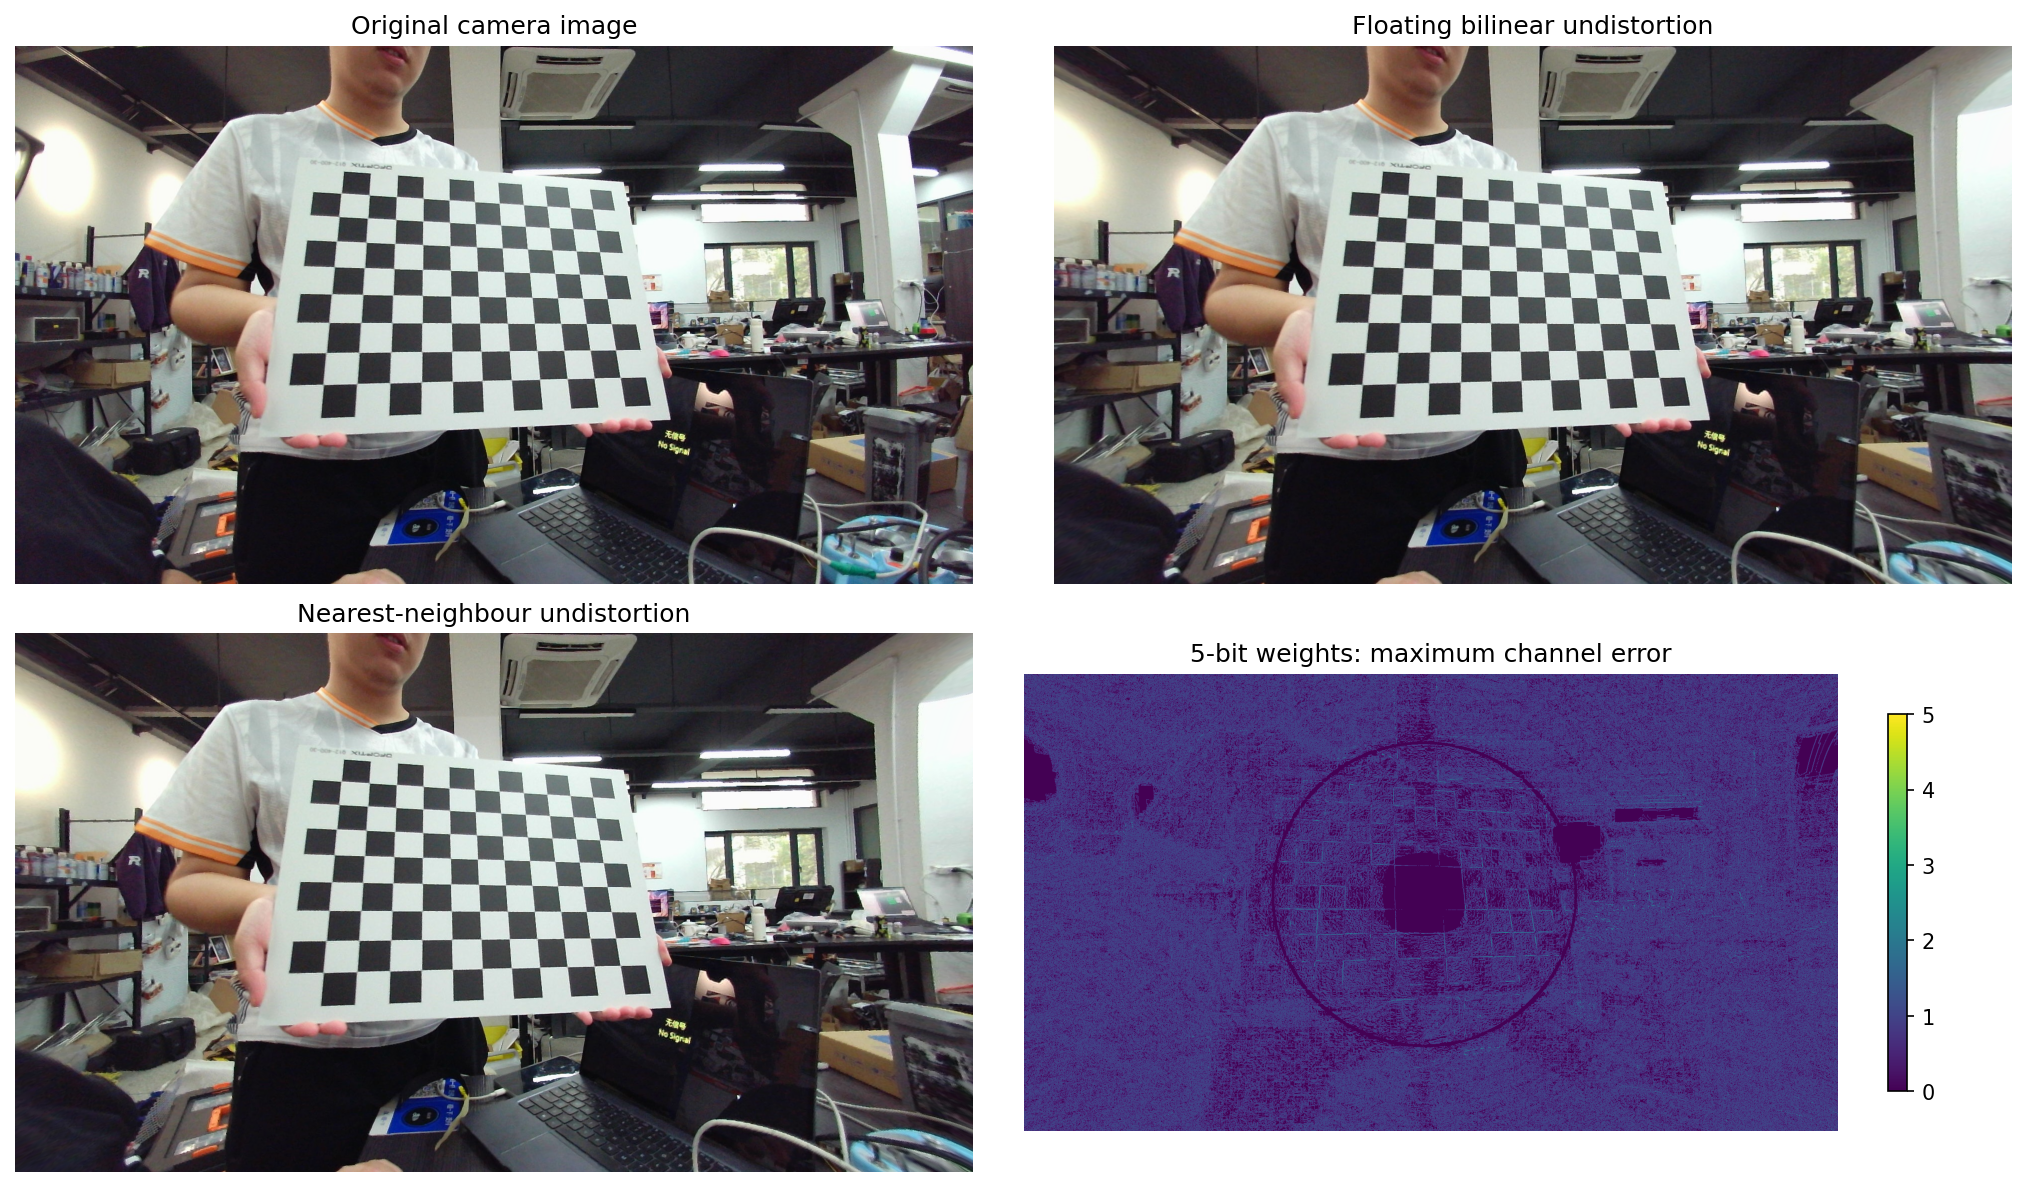
\includegraphics[width=\textwidth]{chapter3/figures/undistort_comparison_reference.png}
\caption{真实相机图像的去畸变与插值对比（独立数值交叉检查生成）}
\label{fig:undistort-simulation}
\end{figure}

\section{姿态矫正算法}
\subsection{参考视线到源相机视线的变换}
镜头去畸变并不能消除相机方向变化引起的透视变化，
因此还需建立参考视场与当前相机视场之间的旋转关系。
本章定义相机坐标轴为 $x$ 向右、$y$ 向下、$z$ 向前，
以 yaw 角 $\psi$ 和 pitch 角 $\theta$ 描述工程使用的两个姿态自由度。
相应旋转矩阵为
\begin{equation}
R_y(\psi)=\begin{bmatrix}
\cos\psi&0&\sin\psi\\0&1&0\\-\sin\psi&0&\cos\psi
\end{bmatrix},\qquad
R_x(\theta)=\begin{bmatrix}
1&0&0\\0&\cos\theta&-\sin\theta\\0&\sin\theta&\cos\theta
\end{bmatrix}.
\end{equation}
按实际算法的运算顺序，输出参考视线先进行 yaw 变换，再进行 pitch 变换，故
\begin{equation}
\boldsymbol d_s=R\boldsymbol d_o,\qquad R=R_x(\theta)R_y(\psi).
\label{eq:pose-rotation}
\end{equation}
若 $C$ 表示源相机坐标到参考坐标的姿态矩阵，则
$C=R^{\mathsf T}=R_y(-\psi)R_x(-\theta)$。
区分 $C$ 与 $R$ 可以避免将相机物理旋转直接当作逆采样方向。

令 $\boldsymbol d_o=[x,y,1]^{\mathsf T}$，先计算
\begin{align}
X_1&=\cos\psi\,x+\sin\psi,&Y_1&=y,&Z_1&=-\sin\psi\,x+\cos\psi,
\end{align}
再计算
\begin{align}
X_s&=X_1,\\
Y_s&=\cos\theta\,Y_1-\sin\theta\,Z_1,\\
Z_s&=\sin\theta\,Y_1+\cos\theta\,Z_1.
\end{align}
透视归一化后的源相机理想坐标为
\begin{equation}
x_s=X_s/Z_s,\qquad y_s=Y_s/Z_s.
\label{eq:pose-normalize}
\end{equation}
当 $Z_s$ 接近零或为负时，视线不具备稳定的前向投影，应判为无效。

\subsection{单应关系与姿态、镜头补偿的组合}
仅考虑相机绕光心旋转且暂不考虑镜头畸变时，有
\begin{equation}
\lambda\boldsymbol p_s=H\boldsymbol p_o,\qquad
H=K_sRK_o^{-1}.
\label{eq:pose-homography}
\end{equation}
本系统中 $K_s=K_o=K$。由于存在齐次除法，yaw/pitch 引起的变换一般是投影变换，
不能直接用二维平移或一般仿射近似替代整个视场的映射。
纯旋转模型不依赖场景深度；如果云台转轴偏离光心而产生明显平移，
不同深度目标会出现视差，该模型无法同时消除所有视差。

组合补偿的计算顺序为
\begin{equation}
\boldsymbol p_o\ \xrightarrow{K_o^{-1}}\ \boldsymbol d_o
\ \xrightarrow{R}\ \boldsymbol d_s
\ \xrightarrow{\text{透视归一化}}\ (x_s,y_s)
\ \xrightarrow{\text{镜头模型}}\ (x_d,y_d)
\ \xrightarrow{K_s}\ (u_s,v_s).
\end{equation}
即将式~\eqref{eq:pose-normalize} 的结果代入镜头模型，最后只进行一次图像重采样。
这也说明不能直接在畸变像素平面上套用理想相机的单应矩阵。

\subsection{姿态输入、有效域与 MATLAB 实验}
工程姿态量按每弧度 2048 个整数单位传送，解码关系为
\begin{equation}
\psi=q_\psi/2048,\qquad\theta=q_\theta/2048.
\end{equation}
当前 FPGA 分块通路的每轴限幅约为 $\pm15^\circ$，roll 不参与变换。
MATLAB 使用双精度三角函数，并单独比较角度量化前后的坐标，
用以分析姿态输入量化误差；它并未模拟 RTL 的每一级截断和查表误差。

\path{run_pose_simulation.m} 构造已知的彩色网格参考平面，
先用 $R^{\mathsf T}$ 合成当前相机图像，再用 $R$ 进行矫正。
该实验关闭镜头畸变以单独考察旋转关系，测试零姿态、单轴转动、双轴组合及边界角度。
理论检查将程序得到的源坐标经式~\eqref{eq:pose-homography} 的逆变换投回，
统计与原输出坐标的差异；图像检查则统计两次采样后与参考图的 RGB 误差。
两者分别反映几何一致性和离散重采样损失，不能混为同一精度指标。

\begin{figure}[htbp]
\centering
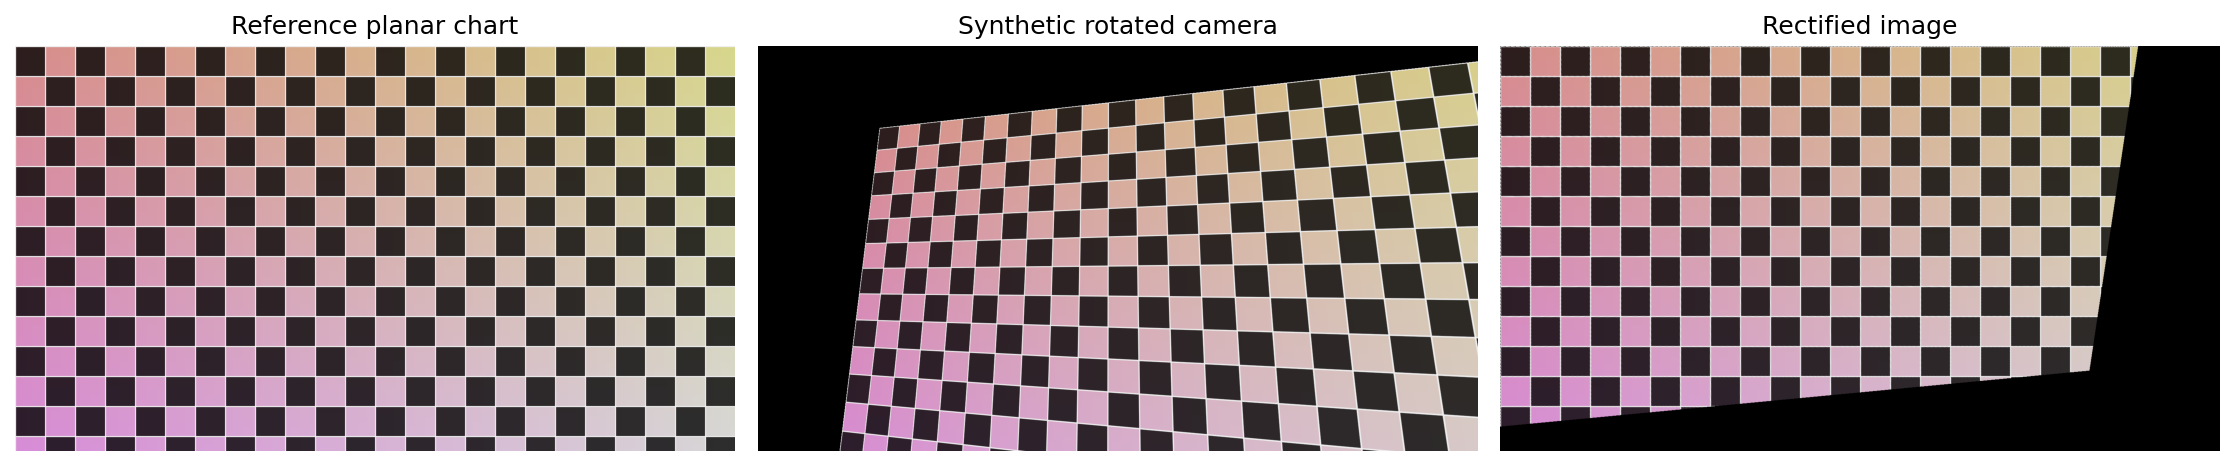
\includegraphics[width=\textwidth]{chapter3/figures/pose_correction_reference.png}
\caption{已知参考网格、合成相机图像与姿态矫正结果（独立数值交叉检查生成）}
\label{fig:pose-simulation}
\end{figure}

统计图像误差时，仅使用输入与合成图像共同可见、且四个插值邻点均有效的区域。
视场外像素置黑，不能把填黑区域当作真实图像参与误差评价。
这类合成实验验证数学映射关系，物理云台的轴向、IMU 零点与时间同步仍需单独实测。

\section{图像重采样及通用处理方法}
\subsection{最近邻与双线性插值}
源坐标 $(u_s,v_s)$ 通常不是整数。最近邻采样选择最近像素，
\begin{equation}
I_o(u,v)=I_s\left(\left\lfloor u_s+\tfrac12\right\rfloor,
\left\lfloor v_s+\tfrac12\right\rfloor\right),
\end{equation}
上式采用图像坐标书写，程序数组索引仍为先行后列。
最近邻实现简单、读取次数少，但会在斜边与细纹理处产生明显的锯齿或跳变。

双线性插值先沿水平方向对相邻两个像素作线性插值，再沿竖直方向插值。
设 $i=\lfloor u_s\rfloor$、$j=\lfloor v_s\rfloor$，
$\alpha=u_s-i$、$\beta=v_s-j$，则
\begin{align}
I_o={}&(1-\alpha)(1-\beta)I_s(i,j)
+\alpha(1-\beta)I_s(i+1,j)\notag\\
&+(1-\alpha)\beta I_s(i,j+1)
+\alpha\beta I_s(i+1,j+1).
\label{eq:bilinear}
\end{align}
四个权重非负且和为 1，因此常值图像应保持不变，线性灰度平面在内部区域可以精确重建。
双线性插值能改善局部连续性，但也可能使高频细节变软，
其效果应结合斜边和纹理区域评价，不能仅凭观感认定清晰度提高。

\subsection{权重量化与整数累加}
为研究有限精度影响，设置 $F=2^b$，将小数位置量化为
\begin{equation}
a=\operatorname{round}(F\alpha),\qquad
b_q=\operatorname{round}(F\beta).
\end{equation}
将式~\eqref{eq:bilinear} 的四个权重改写为整数乘积，先计算
\begin{align}
A={}&(F-a)(F-b_q)I_{00}+a(F-b_q)I_{10}\notag\\
&+(F-a)b_qI_{01}+ab_qI_{11},
\end{align}
再取 $I_o=\lfloor A/F^2\rfloor$。
原仿真使用 $b=5$，故最后除以 $2^{10}$ 可由移位完成。
量化值允许等于 $F$，因此权重在程序中不能被误当作只能表示 $0\ldots F-1$ 的整数。
仿真还保留浮点权重并在输出处取整的参考路径，二者差异包含权重量化和最终舍入规则的影响。

\subsection{边界、有效掩码与颜色处理}
对不在源图像闭区间 $[1,W]\times[1,H]$ 内的坐标，默认输出黑色并记录无效掩码。
对恰好位于末行或末列的有效坐标，重复边界邻点完成退化的一维插值，
从而保证零变换可以完整保留原图。另提供边界复制模式用于方案比较，
但该模式会把边缘内容延伸到视场外，不能视为恢复了未采集的信息。

有效掩码应来自映射与采样条件，不能根据输出 RGB 是否为零判断，
因为图像本身也可能包含黑色目标。
数值保护还限制相机后方视线及径向模型的过度外推。
共用参考函数的深度阈值取 $1024/2^{18}$，径向支持上限取 $r^2\leq600000/2^{18}$，
与工程数值保护保持联系；该上限是算法支持域，不代表独立测得的镜头视场。

RGB 三个通道使用同一组坐标和权重分别插值。
本章参考保留 RGB888，用于观察算法与采样误差；硬件帧缓存采用 RGB565，
比较硬件输出时还应单独考虑颜色量化。
误差统计统一限定到共同有效区域 $\Omega$，例如
\begin{equation}
E_{\rm RGB}=\sqrt{\frac{1}{3|\Omega|}
\sum_{(u,v)\in\Omega}\sum_{c\in\{R,G,B\}}
\left(I_o^{(c)}(u,v)-I_{\rm ref}^{(c)}(u,v)\right)^2}.
\end{equation}
几何坐标误差则以像素为单位，按二维坐标距离计算，不能与灰度级误差直接比较。

\section{帧自适应 Gamma 矫正算法}
\subsection{Gamma 变换与查找表}
将 8 位像素 $z$ 归一化为 $s=z/255$，本系统直接以指数 $\gamma$ 定义变换
\begin{equation}
T_\gamma(z)=\operatorname{round}\left[255\left(\frac{z}{255}\right)^\gamma\right].
\label{eq:gamma-transform}
\end{equation}
这里的指数就是 $\gamma$，没有另取其倒数。
当 $0<\gamma<1$ 时提升中低灰度，当 $\gamma>1$ 时压低中间灰度，
$\gamma=1$ 时保持恒等映射。端点 0 和 255 保持不变，映射单调，
但无法恢复曝光时已饱和或被噪声淹没的细节。

本系统设置七档指数
\begin{equation}
\gamma_c\in\{0.50,0.65,0.80,1.00,1.25,1.55,1.90\},
\qquad c=0,1,\ldots,6.
\end{equation}
每档预先生成 256 项查找表，RGB 三通道共用同一条曲线并独立查表。
对三个通道分别施加非线性变换仍可能改变通道比值和饱和度，
因此增强评价除平均亮度外还应观察颜色表现。

\begin{figure}[htbp]
\centering
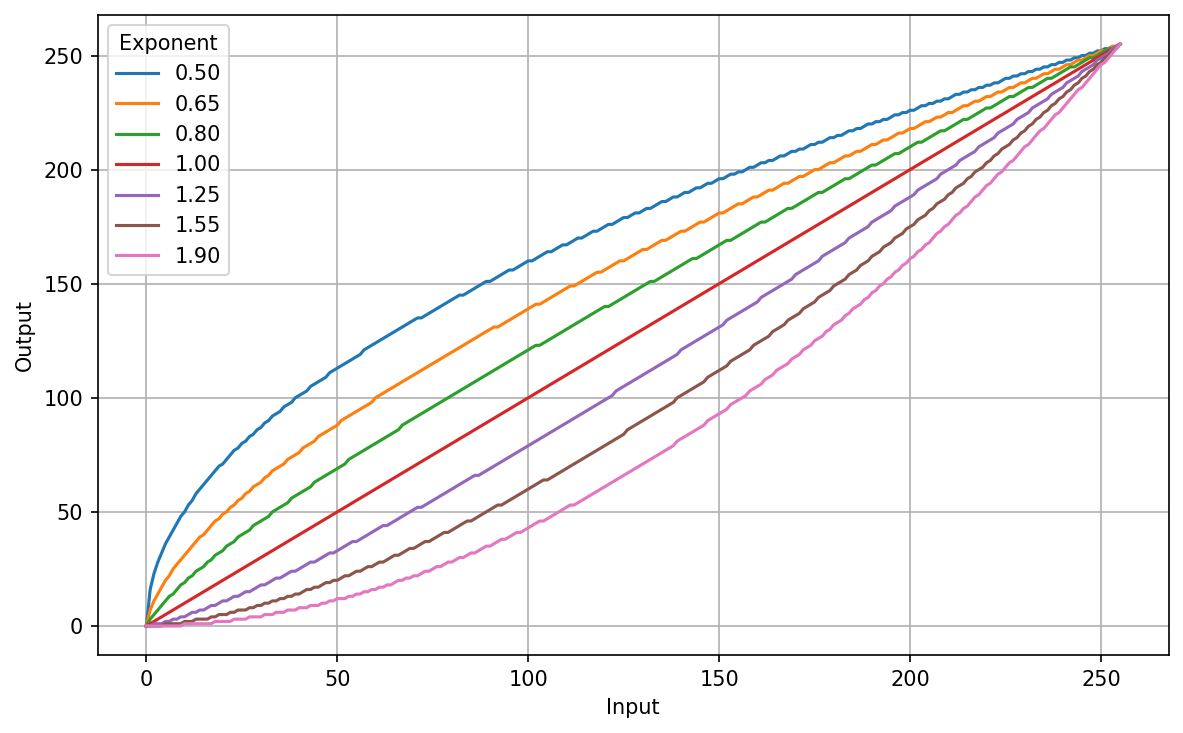
\includegraphics[width=0.76\textwidth]{chapter3/figures/gamma_curves_reference.png}
\caption{七档 Gamma 像素映射曲线（独立数值交叉检查生成）}
\label{fig:gamma-curves}
\end{figure}

\subsection{原始亮度统计与曲线选择}
为降低硬件统计代价，用整数近似亮度
\begin{equation}
Y=\left\lfloor\frac{R+2G+B}{4}\right\rfloor.
\end{equation}
只统计有效图像像素，定义帧像素数 $N$、亮度和 $S$、暗像素数 $D$ 和高光像素数 $H$：
\begin{equation}
S=\sum Y,\qquad D=\sum\mathbf1(Y<48),\qquad H=\sum\mathbf1(Y\geq208),
\qquad\mu=S/N.
\end{equation}
统计对象始终为增强前的原始输入，避免输出亮度改变后反过来驱动选档而形成振荡。
若 $D/N\geq1/8$ 且 $H/N\geq1/8$，优先判为混合光照，选择 $c=2$，
采用温和的暗部提升；否则按表~\ref{tab:gamma-classification} 选择候选曲线。

\begin{table}[htbp]\centering\small
\caption{非混合光照场景的 Gamma 选档规则}
\label{tab:gamma-classification}
\begin{tabular}{ccc}
\toprule
原始帧平均亮度 $\mu$ & 曲线编号 $c$ & 指数 $\gamma_c$\\
\midrule
$\mu<48$ & 0 & 0.50\\
$48\leq\mu<80$ & 1 & 0.65\\
$80\leq\mu<112$ & 2 & 0.80\\
$112\leq\mu\leq144$ & 3 & 1.00\\
$144<\mu\leq176$ & 4 & 1.25\\
$176<\mu\leq208$ & 5 & 1.55\\
$208<\mu$ & 6 & 1.90\\
\bottomrule
\end{tabular}
\end{table}

硬件中不必实际求平均值或比例，例如 $\mu<48$ 改写为 $S<48N$，
混合光照条件改写为 $8D\geq N$ 且 $8H\geq N$，
可利用常数乘法、移位和比较完成。

\subsection{跨帧确认与平滑切换}
为抑制图像内容变化带来的亮度闪烁，系统要求连续两帧得到相同候选分类后，
才更新目标曲线；实际曲线在每个帧起点最多向目标移动一档，且整帧固定。
令 $c_n$ 为第 $n$ 帧的候选分类，$a_n$ 为该帧使用的实际曲线，
$t_n$ 为第 $n$ 帧起点完成上一帧分类后的目标，则
\begin{align}
a_n&=a_{n-1}+\operatorname{sgn}(t_{n-1}-a_{n-1}),\\
t_n&=\begin{cases}
c_{n-1},&c_{n-1}=c_{n-2}\text{ 且两个分类均有效},\\
t_{n-1},&\text{其他情况}.
\end{cases}
\end{align}
初始实际曲线与目标曲线均为 3，即恒等映射。
第 $n-1$ 帧统计在第 $n$ 帧开始时才完整可用，
且该帧实际曲线已按旧目标锁定，新目标最早影响第 $n+1$ 帧。
例如从启动起连续输入暗图，前六帧实际曲线依次为 $3,3,3,2,1,0$。
MATLAB 模型保留这一因果顺序，不用当前帧的全图统计提前处理当前帧。

\subsection{自适应 Gamma MATLAB 仿真}
\path{run_gamma_simulation.m} 以真实图像为基础，构造正常、暗光、强光及左右混合光照
四种受控测试输入，每种连续输入 10 帧，记录原始与增强后平均亮度、候选、目标和实际曲线。
为减少实验开销，仅在这个无几何变换的实验中对图像作四倍间隔抽样。
这些输入用于测试响应机制，不等同于真实低照度传感器噪声或自动曝光过程。

\begin{figure}[htbp]
\centering
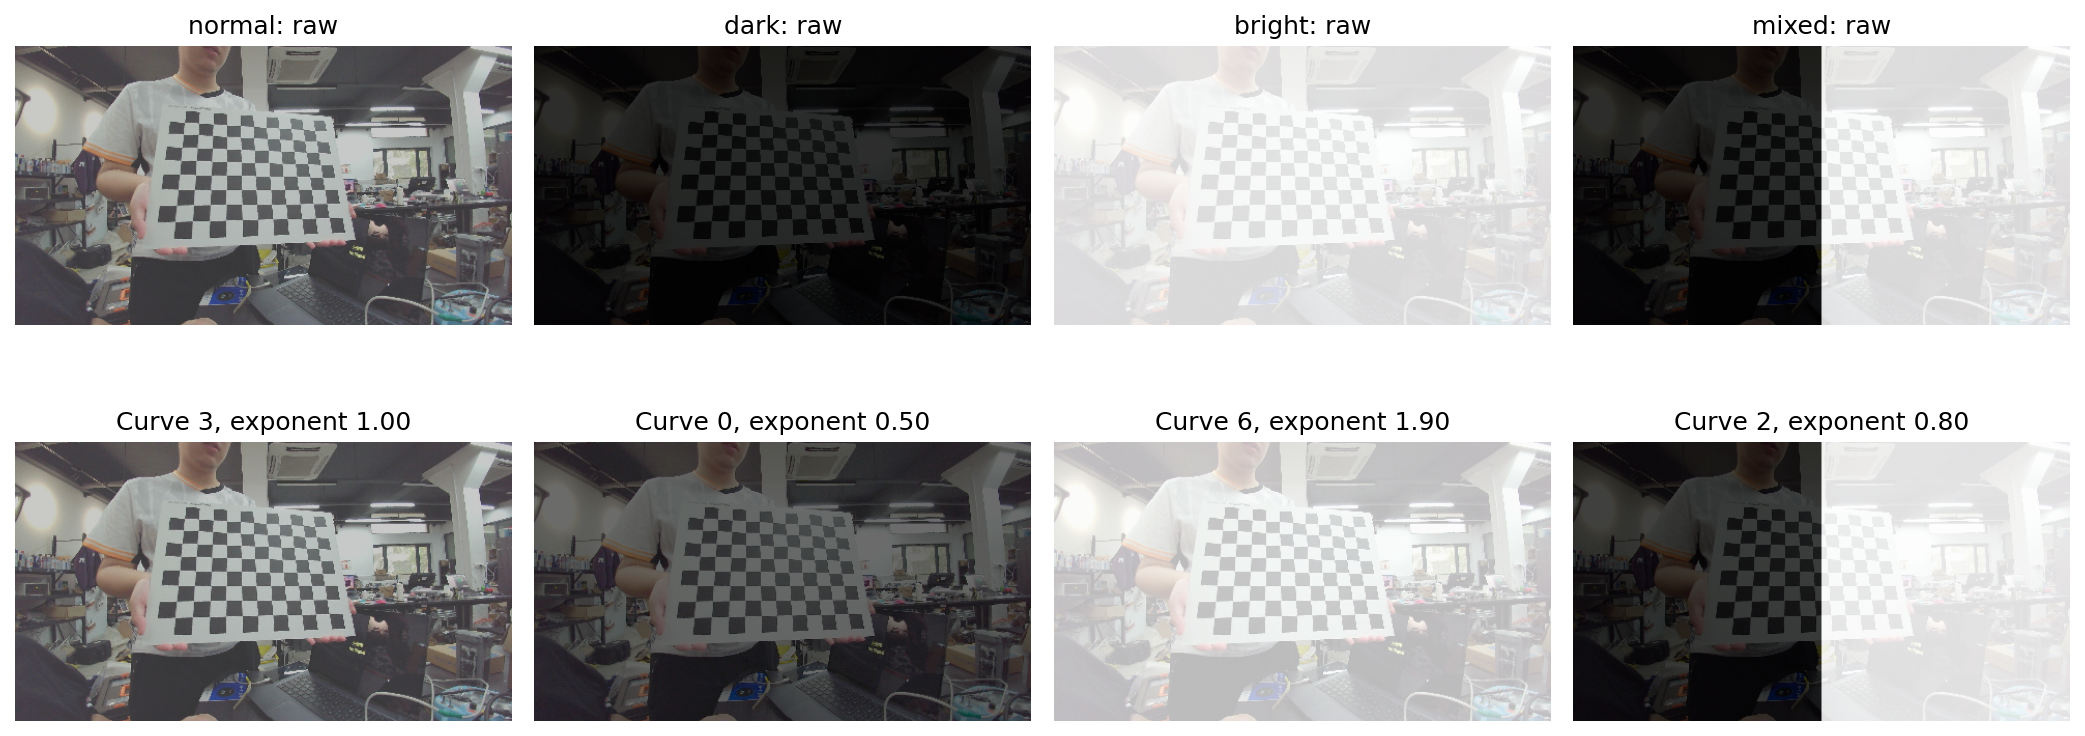
\includegraphics[width=\textwidth]{chapter3/figures/gamma_scenes_reference.png}
\caption{四种受控光照场景及稳定后的增强效果（独立数值交叉检查生成）}
\label{fig:gamma-scenes}
\end{figure}

\begin{figure}[htbp]
\centering
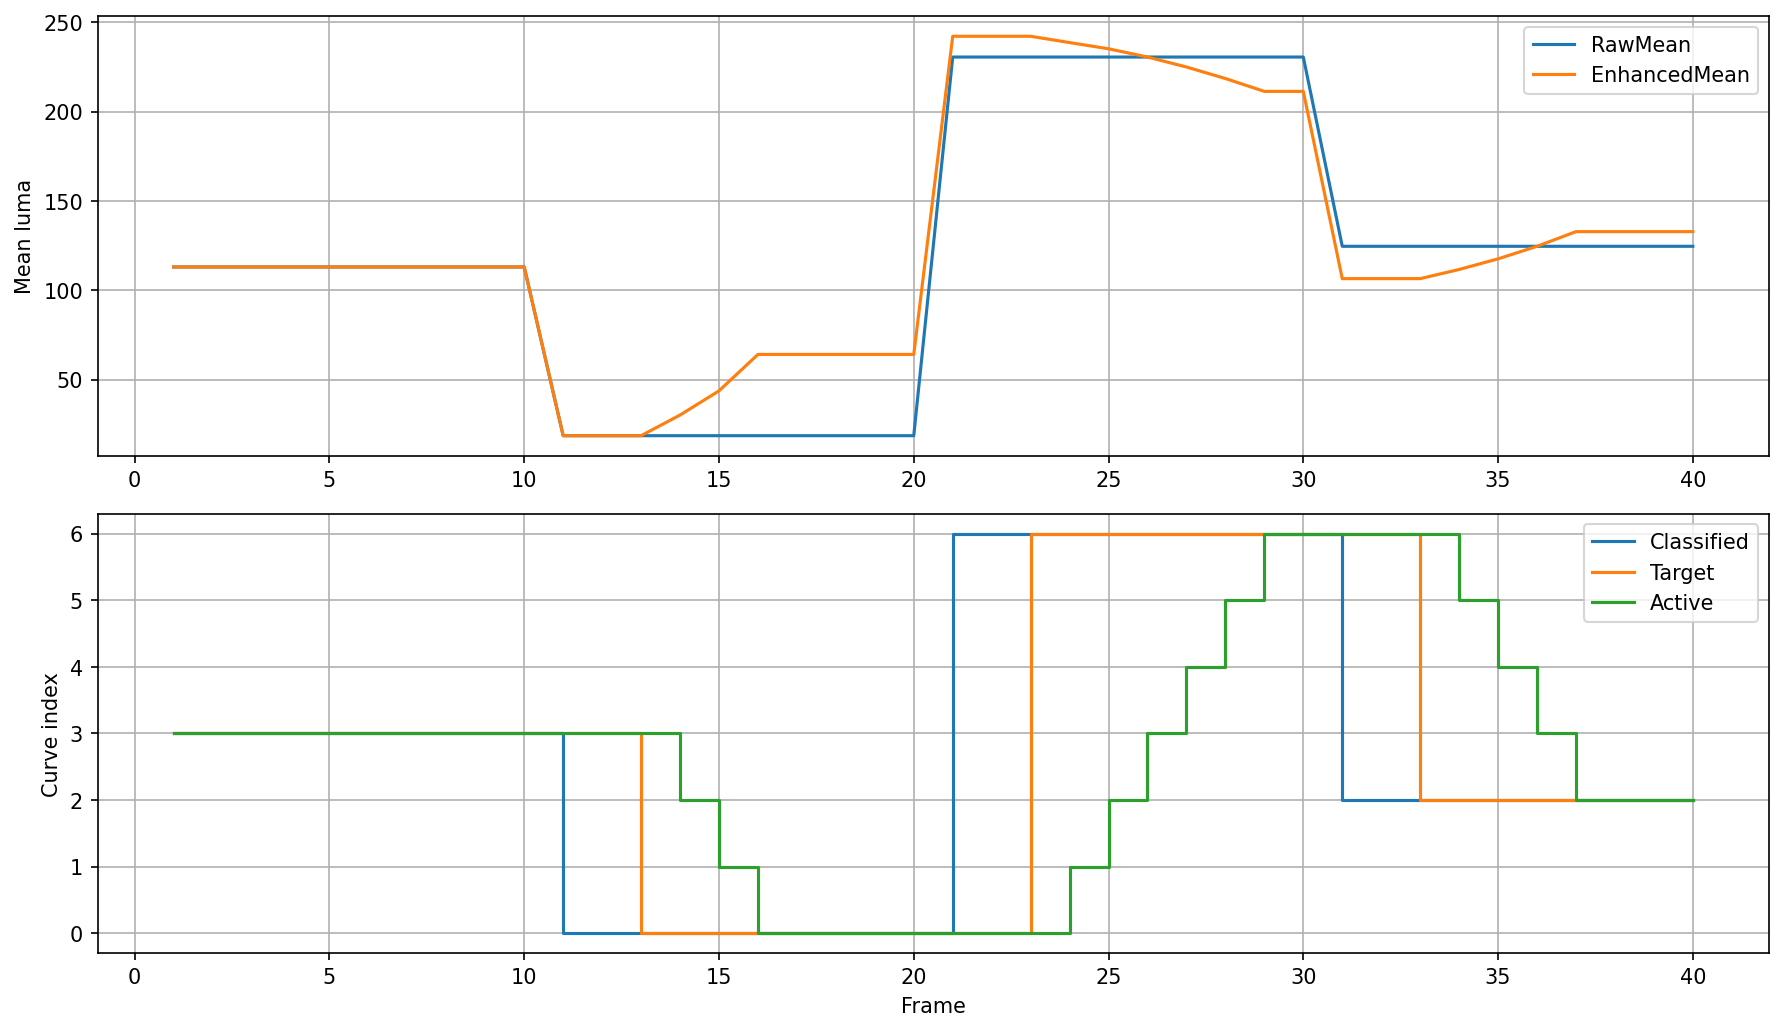
\includegraphics[width=0.9\textwidth]{chapter3/figures/gamma_transition_reference.png}
\caption{亮度统计与曲线切换的帧序列（独立数值交叉检查生成）}
\label{fig:gamma-transition}
\end{figure}

\section{仿真代码组织与结果分析}
\subsection{目录与复现入口}
所有 MATLAB 仿真位于 \path{chapter3/reference/}，
共用参数只在 \path{common/simulation_config.m} 中定义，主要文件见表~\ref{tab:matlab-files}。
输入图像与标定文本作为固定实验数据，计算结果保存于 \path{results/}，
报告插图保存于 \path{chapter3/figures/}。

\begin{table}[htbp]\centering\small
\caption{MATLAB 仿真程序组织}
\label{tab:matlab-files}
\begin{tabularx}{\textwidth}{>{\raggedright\arraybackslash}p{8.5cm}Y}
\toprule
文件（相对于 \path{chapter3/reference/}） & 功能\\
\midrule
\path{run_all_simulations.m} & 三个算法的统一运行入口\\
\path{check_simulation_models.m} & 解析样例、边界和控制时序检查\\
\path{common/inverse_camera_map.m} & 姿态与镜头模型的组合坐标映射\\
\path{common/sample_image.m} & 最近邻、浮点和量化双线性采样\\
\path{common/pose_rotation.m} & 姿态旋转矩阵\\
\path{common/adaptive_gamma_frame.m} & 带历史状态的因果帧级 Gamma 模型\\
\path{undistort/run_undistort_simulation.m} & 去畸变及插值精度比较\\
\path{pose/run_pose_simulation.m} & 合成图卡、姿态扫描及角度量化实验\\
\path{gamma/run_gamma_simulation.m} & 复杂光照与帧间响应实验\\
\bottomrule
\end{tabularx}
\end{table}

在报告根目录启动 MATLAB 后执行：
\begin{verbatim}
addpath('chapter3/reference');
run_all_simulations;
\end{verbatim}
核心算法只依赖 MATLAB 基础数组、图像读写和绘图功能；
内置去畸变比较需要 Computer Vision Toolbox，
保留的图卡质量评估函数还依赖 Image Processing Toolbox。
没有相应工具箱时，手工模型仍可运行，内置比较按可用性跳过。

\subsection{独立数值验证结果}
算法参考程序 \path{verify_reference.py} 使用 SciPy 插值和矩阵运算，
对几何映射、颜色重采样与 Gamma 控制关系进行独立数值验证。
本章图示与数值均来自该程序；MATLAB 程序提供同模型复现入口，
未列入已执行的 MATLAB 测试结果，数值验证也不作为 FPGA 实板测量。

在 $1920\times1080$ 测试图像上，零姿态去畸变映射的有效区域占比为 100\%，
该比例描述既定参数与输出视场下的坐标覆盖。
5 位权重双线性与浮点双线性的最大通道差为 5 灰度级，RGB 均方根差约为 0.677 灰度级。
该结果反映插值权重及取整差异，不能据此代替镜头标定精度或图像清晰度指标。

在 yaw 为 $10^\circ$、pitch 为 $-8^\circ$ 的合成图卡实验中，
共同有效区域约占 73.83\%，两次采样后的 RGB 均方根误差约为 8.88 灰度级。
六组姿态的连续坐标往返误差低于 $10^{-9}$ 像素，
而仅对输入角度作 Q2048 量化后，该双轴场景的源坐标均方根变化约为 0.239 像素。
这说明连续几何一致性、姿态量化和图像插值损失应分别评价。

在稳定后的暗光测试段，平均亮度从约 18.67 提升至 64.14；
强光段从约 230.51 降至 211.30；混合光照选择指数为 0.80 的温和曲线。
七档曲线及安全恒等档的 2048 项数值与 FPGA Gamma ROM 一致，
帧间实际曲线变化也满足每帧至多一档的约束。
这些结果验证了模型的数值关系与控制逻辑，最终画质、颜色、动态姿态同步及硬件吞吐
分别在后续硬件与测试章节中评价。

\chapter{FPGA 代码设计与实现}
\label{chap:hardware}

\tikzset{
  fpblock/.style={draw=TemplateBlue,rounded corners=2pt,fill=TemplateGray,
    align=center,font=\fontsize{9.5}{12.5}\selectfont,minimum height=10mm,text width=4cm,inner sep=4pt},
  fpstate/.style={fpblock,text width=3.1cm},
  fparrow/.style={-{Stealth[length=2mm]},thick,draw=TemplateBlue},
  fpnote/.style={align=center,font=\fontsize{8.5}{11}\selectfont,text=TemplateBlue}
}

\section{设计范围与 RTL 总体结构}
本章以 \path{../Pgl50h/EmbFPGA.pds} 登记的工程及
\path{src/top/hdmi_ddr3_top.v} 默认参数为依据，说明第三章算法在
PGL50H-FBG484-6 上的 RTL 实现。系统输入、输出均为
$1920\times1080$、60 Hz 的 HDMI 视频，外部并行接口采用 RGB888，
DDR3 内的源帧和结果帧采用 RGB565。算法按完整源帧调度，显示端按独立光栅连续扫描，
两者通过结果帧槽解耦；60 Hz 输出时序本身不代表每秒产生 60 个不同的矫正结果。

默认参数为 \path{UNDISTORT_ENABLE=1}、\path{POSE_CORRECTION_ENABLE=1}、
\path{POSE_TILED_ENABLE=1}、\path{INTERPOLATION_MODE=1}，
即启用双槽分块逆投影与最近邻采样。输入预处理选择
\path{ADAPTIVE_PREPROCESS_MODE=3}，启用帧自适应 Gamma；
\path{PC_CONTROL_ENABLE=1} 支持运行时控制。
\path{POSE_RECIPROCAL_LUT_ENABLE=0} 选择恢复除法流水线，
\path{OUTPUT_BYPASS=0} 选择处理后输出。
双线性插值由保留的串行路径实现，不属于本章默认分块数据通路。

图~\ref{fig:fpga-architecture} 给出按实际实例关系整理的 RTL 结构原理图。
图中的 DDR3 控制器以及时钟通路使用的 PLL 采用厂商 IP；
像素处理、帧管理和仲裁功能由工程 RTL 实现。
\begin{figure}[htbp]
\centering
\begin{tikzpicture}
\node[fpblock] (rx) at (0,0) {MS7200 并行输入\\RGB888、DE、VS};
\node[fpblock] (gamma) at (5,0) {输入寄存 + 自动 Gamma\\\texttt{pixclk\_in}};
\node[fpblock] (capture) at (10,0) {RGB565 / 完整帧采集\\打包 → 采集异步 FIFO};
\node[fpblock] (render) at (0,-2.3) {双槽分块渲染器\\联合逆投影 / 源缓存 / 采样};
\node[fpblock] (arb) at (5,-2.3) {DDR 读写仲裁器\\采集/渲染写，显示/渲染读};
\node[fpblock] (ddr) at (10,-2.3) {\texttt{DDR3\_50H} IP\\用户数据 256 bit / DDR3};
\node[fpblock] (display) at (0,-4.6) {结果帧预取 / 显示 FIFO\\RGB565 解包};
\node[fpblock] (output) at (5,-4.6) {RGB888 展开 / 输出寄存\\独立 1080p60 光栅};
\node[fpblock] (tx) at (10,-4.6) {MS7210 并行输出\\RGB888、DE、HS、VS};
\draw[fparrow] (rx)--(gamma);
\draw[fparrow] (gamma)--(capture);
\draw[fparrow] (capture.south)--++(0,-0.65)-| (arb.north);
\draw[fparrow] (arb.east)--(ddr.west);
\draw[fparrow] (ddr.south)--++(0,-0.45)-| (arb.south east);
\draw[fparrow,<->] (render.east)--(arb.west);
\draw[fparrow] (arb.south)--++(0,-0.65)-| (display.north);
\draw[fparrow] (display)--(output);
\draw[fparrow] (output)--(tx);
\node[fpnote] at (0,-1.2) {帧级锁存 IMU 姿态与几何开关};
\node[fpnote] at (10,0.95) {PC 掩码在输入 SOF 应用};
\node[fpnote] at (5,-5.6) {帧槽管理、采集、渲染和显示预取由 \texttt{fram\_buf\_pose} 组织};
\end{tikzpicture}
\caption{默认配置的 RTL 数据通路结构原理图（按源码连接重绘）}
\label{fig:fpga-architecture}
\end{figure}


\begin{longtable}{p{6.0cm}p{9.0cm}}
\caption{默认数据通路中的主要模块及职责}\label{tab:modules}\\
\toprule 模块（相对 \path{src/}） & 实现职责 \\\midrule\endfirsthead
\toprule 模块（相对 \path{src/}） & 实现职责 \\\midrule\endhead
\bottomrule\endfoot
\path{top/hdmi_ddr3_top.v} & 连接板级接口、PLL、DDR3 IP、视频处理和控制通路；按参数选择生成分支。\\
\path{board/ms72xx_ctl.v} & 组织 MS7200、MS7210 的寄存器初始化及两路 I\textsuperscript{2}C 接口。\\
\path{video/preprocess/adaptive_gamma_stream.v} & 原始帧亮度统计、目标曲线选择、三通道同步 LUT 查询及旁路对齐。\\
\path{video/format/rgb888_to_rgb565.v} & 对齐 VS、DE 与 RGB，寄存输出 RGB565 写接口。\\
\path{video/pose/fram_buf_pose.v} & 完整源帧采集、帧槽分配、姿态快照、渲染启动、结果发布与显示读出。\\
\path{video/pose/pose_renderer_tiled.v} & 双块槽调度、逐像素投影、源区域预取、最近邻采样及结果突发写回。\\
\path{video/pose/pose_inverse_project_q14.v} & 帧姿态系数准备、定点逆投影、镜头模型及坐标有效性判定。\\
\path{video/pose/pose_ddr_arbiter.v} & 两个写客户端、两个读客户端共享 DDR3 用户接口；核验长度、ID 和 LAST。\\
\path{video/pose/pose_async_fifo.v} & 采集和显示数据的双时钟缓冲，含同步 RAM 预取与 Gray 指针同步。\\
\path{video/timing/sync_vg.v}、\path{video_raster_delay.v} & 独立生成 1080p60 光栅，延迟显示 DE；二者位于同一目录。\\
\path{video/format/rgb565_to_rgb888.v}、\path{video/preprocess/gamma_correct_rgb888.v} & RGB 展开及输出寄存；自动 Gamma 模式关闭后级固定 Gamma 运算。\\
\path{imu/imu_protocol_50m.v}、\path{imu/attitude_cdc.v} & IMU 串口解析及姿态快照跨域。\\
\path{control/cp2102_control.v}、\path{control/video_control_cdc.v} & PC 协议解析、串口应答及输入帧边界应用控制掩码。\\
\path{control/gamma_telemetry.v}、\path{control/cdc_snapshot.v} & 形成同帧统计快照，握手跨域后发送遥测。\\
\end{longtable}
工程还保留线性帧缓存、单独去畸变及串行姿态矫正等生成分支。
独立文件 \path{pose_frame_bank_allocator.v} 和 \path{pose_tile_read_scheduler.v}
虽登记在工程中，默认路径未实例化；本章的帧槽、块读取调度分别对应
\path{fram_buf_pose.v} 和 \path{pose_renderer_tiled.v} 内部逻辑。
\sourcefile{\path{../Pgl50h/EmbFPGA.pds}；\path{../Pgl50h/src/top/hdmi_ddr3_top.v}}

\section{顶层接口、时钟与启动控制}
\subsection{顶层端口及接口边界}
表~\ref{tab:fpga-top-ports} 中方向均相对于 FPGA。
视频接口使用 DE 指示有效像素，输入 HS 不参与默认路径的逐行地址计数；
完整帧内有效像素按 DE 顺序打包，不进行水平抽列或缩放。
\begin{table}[htbp]\centering\small
\caption{顶层主要物理接口}\label{tab:fpga-top-ports}
\begin{tabularx}{\textwidth}{p{5.3cm}p{1.2cm}Y}
\toprule 端口组及位宽 & 方向 & 含义 \\\midrule
\path{sys_clk}、\path{video_ref_clk} & 输入 & 板载 50 MHz 系统时钟、27 MHz 视频参考时钟。\\
\path{pixclk_in}、\path{vs_in/hs_in/de_in}、\path{r_in/g_in/b_in[7:0]} & 输入 & MS7200 输出的源同步像素总线，1080p60 下约 148.5 MHz。\\
\path{pixclk_out}、\path{vs_out/hs_out/de_out}、\path{r_out/g_out/b_out[7:0]} & 输出 & 驱动 MS7210 的并行视频总线。\\
\path{imu_uart_rx} & 输入 & IMU UART，921600 bit/s、8N1。\\
\path{pc_uart_rx}、\path{pc_uart_tx} & 入/出 & 板载 CP2102 UART，115200 bit/s、8N1。\\
\path{sys_led[7:0]} & 输出 & 低三位依次显示镜头、姿态、Gamma 的已应用使能，其余位为 0。\\
\path{rstn_out}、两路 \path{iic*_scl/sda} & 出/双向 & 桥芯片复位与寄存器配置，SDA 通过三态接口连接。\\
\path{mem_a[14:0]}、\path{mem_ba[2:0]}、命令/时钟端口 & 输出 & DDR3 行列/Bank 地址、差分时钟及命令控制。\\
\path{mem_dq[31:0]}、\path{mem_dqs(_n)[3:0]}、\path{mem_dm[3:0]} & 双向/出 & 32 bit DDR3 物理数据、四组差分数据选通与字节屏蔽。\\
\bottomrule
\end{tabularx}
\end{table}

\subsection{时钟域划分与复位顺序}
系统分为四类工作域，如表~\ref{tab:fpga-clocks} 所示。
输入、输出像素时钟即使标称频率相同，也来自不同信号源，不能直接混用。
\begin{table}[htbp]\centering\small
\caption{实际工作时钟与承载逻辑}\label{tab:fpga-clocks}
\begin{tabularx}{\textwidth}{p{3.0cm}p{3.0cm}Y}
\toprule 时钟域 & 来源与频率 & 承载逻辑 \\\midrule
\path{sys_clk} & 板载 50 MHz & UART 接收/发送、IMU 协议、PC 控制。\\
\path{cfg_clk} & $27\times44/119\approx9.983$ MHz & 启动等待及 MS72xx I\textsuperscript{2}C 配置。\\
\path{pixclk_in} & HDMI 接收像素时钟 & 输入寄存、自动 Gamma、RGB565 打包、源帧姿态锁存。\\
\path{ddr_core_clk} & DDR3 IP 用户时钟 100 MHz & 采集写入、帧槽管理、投影/渲染、DDR 仲裁及显示预取。\\
\path{pixel_clk} & $27\times44/8=148.5$ MHz & 输出光栅、RGB565 解包、输出流水线。\\
\bottomrule
\end{tabularx}
\end{table}
视频 PLL 锁定后，\path{cfg_clk} 域计数至 10000，约等待 1 ms，
再拉高 \path{rstn_out}。\path{ms72xx_ctl} 先完成接收端 MS7200 的配置，
再以接收端完成信号释放 MS7210 配置状态机；两路 I\textsuperscript{2}C
使用独立驱动，按约 400 kHz 参数配置，寄存器地址低字节先发送。
DDR3 IP 同时以 \path{rstn_out} 释放复位并完成校准。

系统、输入像素和输出像素逻辑设置各自的两级复位释放同步寄存器；
帧缓存与异步 FIFO 以 \path{ddr_init_done} 为复位条件，分别在像素域释放。
跨域数据通路只有在相应复位释放且有效标志成立后使用。
输出光栅由 \path{video_reset_n} 控制，独立于 DDR 校准和首帧完成状态运行，
因此初始化尚未完成时仍能提供标准行场时序，并用诊断颜色表示状态。

\section{视频输入、自适应 Gamma 与输出时序}
\subsection{固定延迟的输入数据通路}
默认输入通路如图~\ref{fig:fpga-gamma}。
原始 RGB、DE 和低有效 VS 首先在 \path{pixclk_in} 上升沿寄存；
送入自动 Gamma 时将 VS 取反，以高有效 VS 的上升沿表示帧起始 SOF。
Gamma 的两个寄存级同时处理 RGB、完整 VS 电平和 DE，
再由 \path{rgb888_to_rgb565} 寄存成写接口。总计四拍输入延迟，
其中格式转换为
\begin{equation}
P_{565}=\{R[7:3],\ G[7:2],\ B[7:3]\}.
\end{equation}
格式转换输出 \path{wr_en}、\path{wr_data[15:0]} 和 \path{vs_out}
进入帧缓存；SOF 在帧缓存入口恢复为高有效 \path{wr_fsync}。
Gamma 关闭时使用同延迟旁路，保证开关前后帧同步与像素位置不变。
\begin{figure}[htbp]
\centering
\begin{tikzpicture}
\node[fpblock] (in) at (0,0) {输入 I/O 寄存\quad 1 拍\\RGB888、DE、VS};
\node[fpblock] (lut) at (5,0) {Gamma 寄存 / 同步 LUT\\RGB、DE、VS 共 2 拍};
\node[fpblock] (convert) at (10,0) {RGB888 → RGB565\quad 1 拍\\\texttt{wr\_data / wr\_en / VS}};
\node[fpblock] (stats) at (0,-2.3) {原始亮度与 DE 统计\\$S,N,N_{\rm dark},N_{\rm high}$};
\node[fpblock] (target) at (5,-2.3) {移位 / 加法阈值比较\\连续两帧相同 → 目标曲线};
\node[fpblock] (active) at (10,-2.3) {SOF 锁存使能 / 活动曲线\\向旧目标每帧移动至多一级};
\draw[fparrow] (in)--(lut);
\draw[fparrow] (lut)--(convert);
\draw[fparrow] (in)--(stats);
\draw[fparrow] (stats)--(target);
\draw[fparrow] (target)--(active);
\draw[fparrow,dashed] (active.north)--(10,-1.1)-| (lut.south);
\node[fpnote] at (5,1.0) {关闭 Gamma 选择同延迟旁路；总输入延迟为 4 拍，启动间隔为 1 拍};
\node[fpnote] at (5,-3.35) {统计在下一 SOF 发布，新分类只能影响后续完整帧；首帧使用恒等曲线};
\end{tikzpicture}
\caption{自适应 Gamma 的像素流水线与帧级控制回路}
\label{fig:fpga-gamma}
\end{figure}


\subsection{Gamma 的统计、控制与 LUT 电路}
\path{adaptive_gamma_stream} 的数据接口为
\path{in_r/g/b[7:0]}、\path{in_de/in_vs} 输入和对应
\path{out_r/g/b[7:0]}、\path{out_de/out_vs} 输出，流水线启动间隔为一拍，
接口不支持输入回压。控制端 \path{enable} 在 SOF 锁存，
输出 \path{active_curve[2:0]}、\path{target_curve[2:0]} 表示曲线状态。

亮度以 $Y=(R+2G+B)\gg2$ 计算，仅对原始输入的 DE 像素累加。
内部亮度和为 30 bit，像素数、暗像素数和高亮像素数为 22 bit，
分别覆盖 1080p 的最大亮度和 528768000 与像素数 2073600。
统计结果在下一帧 SOF 以 \path{stats_valid} 发布，四项统计扩展为 32 bit；
\path{stats_curve/stats_target/stats_enabled} 描述刚完成的统计帧。

曲线选择电路通过亮度和 $S$ 与常数倍像素数 $N$ 比较，避免实时求平均值除法。
在不满足混合光照判据时，按表~\ref{tab:fpga-gamma-select} 选曲线。
若暗像素 $Y<48$ 和高亮像素 $Y\ge208$ 均至少占 $1/8$，优先选择曲线 2。
\begin{table}[htbp]\centering\small
\caption{自动 Gamma 的分类规则及预存指数}\label{tab:fpga-gamma-select}
\begin{tabular}{ccc}
\toprule 分类条件（依次判定） & 曲线编号 & LUT 指数 $\gamma$ \\\midrule
$S<48N$ & 0 & 0.50\\
$48N\le S<80N$ & 1 & 0.65\\
$80N\le S<112N$ & 2 & 0.80\\
$S>208N$ & 6 & 1.90\\
$176N<S\le208N$ & 5 & 1.55\\
$144N<S\le176N$ & 4 & 1.25\\
其余 & 3 & 1.00\\
\bottomrule
\end{tabular}
\end{table}
连续两次分类相同才更新目标曲线；活动曲线仅在 SOF 向当时已有目标移动一级。
当前 SOF 发布的统计稍后才形成新目标，因此不会改变正在开始的这一帧。
复位时活动与目标均为恒等曲线 3。
\path{adaptive_gamma_lut} 按
$\operatorname{round}[255(v/255)^\gamma]$ 预存映射，
地址为曲线号与 8 bit 通道值拼接；每通道实例化一份 $2048\times8$ bit 同步 ROM。
关闭增强仍保留原始统计与曲线状态演进，像素选择延迟匹配的旁路值。
\sourcefile{\path{../Pgl50h/src/video/preprocess/adaptive_gamma_stream.v}；\path{adaptive_gamma_lut.v}}

\subsection{显示读出及行场对齐}
\path{sync_vg} 的行总长为 2200 像素，场总长为 1125 行，
有效区域为 $1920\times1080$；水平前肩/同步/后肩分别为 88/44/148，
垂直分别为 4/5/36。在 148.5 MHz 下，帧率为
$148.5\times10^6/(2200\times1125)=60$ Hz。
默认 \path{alg_rd_en=timing_de}，每个有效扫描位置都请求一个像素。

显示 FIFO 的 256 bit 数据按低位到高位拆成 16 个 RGB565 像素，
\path{fram_buf_pose} 内两拍寄存输出像素。
\path{video_raster_delay} 将光栅 DE 延迟同样的两拍，
\path{rgb565_to_rgb888} 用位复制组合展开到 RGB888，
后级 \path{gamma_correct_rgb888} 即使关闭运算仍保留一拍寄存，
最终顶层输出再寄存一拍。因此默认数据、DE、HS、VS 相对于输出时序源均延迟四拍。
自动 Gamma 生效时后级固定 Gamma 被旁路，避免重复校正。

最终视频寄存器放置在输出 I/O 单元；物理 \path{pixclk_out} 保持正相，
RGB/控制在上升沿更新，MS7210 按下降沿采样。
DE 无效时 RGB 清零；有效期内依优先级输出初始化诊断颜色：
发送端未完成为品红、DDR PLL 未锁定为蓝、DLL 未锁定为青、
DDR 未完成校准为红、尚无完整结果帧为黄，均就绪后输出处理数据。
\sourcefile{\path{../Pgl50h/src/top/hdmi_ddr3_top.v}；\path{../Pgl50h/src/video/timing/}}

\section{完整帧缓存与帧槽所有权}
\subsection{帧缓存接口和 DDR 地址组织}
\path{fram_buf_pose} 将采集、渲染与显示封装为统一帧缓存。
输入域接收 \path{wr_fsync/wr_en/wr_data[15:0]} 和已跨域的
\path{imu_yaw/imu_pitch[15:0]}、\path{lens_enable}；
输出域接收 \path{rd_fsync/rd_en}，返回
\path{vout_de/vout_data[15:0]}；DDR 域输出下节定义的用户命令。
\path{init_done} 在首个结果帧交给显示后置位，
\path{captured_frames/rendered_frames/displayed_frames} 分别计数采集提交、渲染完成和结果发布次数。
这些诊断计数及 \path{protocol_error} 等端口在当前顶层留空，未直接接入 UART 遥测。

一帧的有效数据量为
\begin{equation}
S_f=1920\times1080\times2=4147200\ \text{bytes},\qquad
N_b=\frac{1920\times1080}{16}=129600\ \text{beat}.
\end{equation}
DDR 用户地址以 32 bit word 为单位，一拍 256 bit 占 8 个地址单位，
同一帧相邻行首地址相差 $1920/2=960$。
帧槽 $b$ 的基址及其中像素 $(x,y)$ 所在 beat 地址为
\begin{equation}
A_b=b\,2^{22},\qquad
A(b,x,y)=A_b+960y+8\left\lfloor\frac{x}{16}\right\rfloor.
\label{eq:fpga-ddr-address}
\end{equation}
像素在 beat 内的 lane 为 $x\bmod16$，首像素位于数据低 16 bit。
基址转换为字节地址后如表~\ref{tab:fpga-banks}。
\begin{table}[htbp]\centering\small
\caption{DDR3 帧槽布局}\label{tab:fpga-banks}
\begin{tabular}{cccc}
\toprule 槽号 & 用户地址基址（word） & 字节地址基址 & 用途 \\\midrule
0 & \texttt{0x0000000} & \texttt{0x00000000} & 源帧 A\\
1 & \texttt{0x0400000} & \texttt{0x01000000} & 结果帧 A\\
2 & \texttt{0x0800000} & \texttt{0x02000000} & 结果帧 B\\
3 & \texttt{0x0C00000} & \texttt{0x03000000} & 源帧 B\\
\bottomrule
\end{tabular}
\end{table}
帧槽间隔为 16 MiB，仅有效帧载荷参与传输；DDR 帧槽与后文片内两个块槽是不同层次的缓存。

\subsection{源帧采集、提交与并行调度}
DDR 域翻转 \path{capture_request} 请求一帧，输入域同步该翻转，
在下一个 SOF 才开始采集，并同时锁存 yaw、pitch 和镜头使能。
每收齐 16 个有效像素产生一个 256 bit FIFO 写脉冲。
DDR 域从采集 FIFO 取数，先装满最多 16 beat 的客户端突发 RAM，再提交写命令。
未凑满 16 beat 的尾部在确认采集结束且 FIFO 排空后提交。

输入域收齐 2073600 个像素后发布完成翻转；DDR 域同步完成与失败标志，
再等待 8 个 DDR 时钟，使完成消息和最后一笔 FIFO 写指针均有时间到达。
只有 FIFO 无有效数据、占用计数为零、无未完成采集写、突发缓冲为空，
且已完成写入恰为 129600 beat 时，才接受该源帧。
输入提前出现新 SOF、FIFO 满导致写脉冲未被接受或帧长度不符，均使该帧被丢弃并重新请求。
HDMI 输入不能回压，FIFO 的 \path{wr_ready} 只用于检测接收失败。

默认快速路径的控制状态为
\path{C_REQUEST}（请求采集）、\path{C_CAPTURE}（收集并提交）和
\path{C_RENDER}（完整源帧等待调度）。后者需等待渲染器空闲、无待发布结果且无渲染错误，
再把源帧槽、姿态和镜头使能交给渲染器。
启动后采集槽在 0/3 间切换，下一帧采集与当前帧渲染重叠；
若新源帧已就绪而渲染器仍忙，就保持该源帧，并跳过后续输入帧，直到它可以调度。
\begin{figure}[htbp]
\centering
\begin{tikzpicture}
\node[fpblock] (cap) at (0,0) {源槽采集（0/3 轮换）\\SOF 锁存姿态并接收像素};
\node[fpblock] (ready) at (5,0) {完整源帧等待调度\\FIFO 排空、全部采集写结束};
\node[fpblock] (render) at (10,0) {源槽只读供渲染\\整帧像素与姿态保持不变};
\draw[fparrow] (cap)--(ready);
\draw[fparrow] (ready)--(render);
\draw[fparrow] (render.north)--++(0,0.8)-| (cap.north);
\node[fpnote,fill=white] at (5,1.0) {前一渲染完成后源槽可再次使用；另一源槽可并行采集};
\node[fpblock] (write) at (0,-2.5) {空闲结果槽（1/2 轮换）\\选择当前显示槽以外的槽};
\node[fpblock] (pending) at (5,-2.5) {待发布完整结果\\最后块末行写完成 → done};
\node[fpblock] (show) at (10,-2.5) {显示持有结果槽\\按独立光栅重复读出};
\draw[fparrow] (write)--(pending);
\draw[fparrow] (pending)--(show);
\draw[fparrow] (show.south)--++(0,-0.9)-| (write.south);
\node[fpnote,fill=white] at (5,-3.65) {新结果替换显示槽后，旧显示槽方可写入下一结果};
\node[fpnote,text width=14cm] at (5,-1.2)
 {发布门槛：显示 VS 请求新 epoch → 旧读事务结束 → 旧 FIFO 排空 → 确认与接受握手};
\end{tikzpicture}
\caption{源帧与结果帧的逻辑所有权流转（概念状态，与 RTL 标志及控制状态对应）}
\label{fig:fpga-frame-ownership}
\end{figure}


\subsection{结果发布与显示 epoch 握手}
结果帧始终写入当前显示槽之外的 1/2 号槽。
\path{renderer_done} 且无错误时设置 \path{pending_valid}，表示完整结果已提交。
显示域在 VS 上升沿翻转 \path{display_request}，开始刷新 epoch，停止使用旧像素并排空显示 FIFO。
DDR 域检测到新 epoch 后停止发旧帧读命令，等在途读完成且 FIFO 写域空闲额度恢复为全深度，
才确认 epoch；此时如有待发布结果则切换显示槽，否则继续使用原显示槽。
显示域收到确认后返回 \path{display_accept_epoch}，DDR 域收到此接受消息才允许新一轮预取。
因此旧事务、旧 FIFO 数据均先结束，随后才允许新的帧数据进入。

显示按最多 16 beat 突发预取，发命令前检查 FIFO 空闲额度能够容纳整笔返回。
若有效扫描期间 FIFO 饥饿，置位粘滞诊断 \path{display_underrun}，
并把本帧余下像素补黑、排掉迟到数据，下一帧边界重新交接，避免晚到像素造成水平错位。
\path{displayed_frames} 只在发布新结果时增加，不能用它直接计数全部物理 HDMI 扫描帧。
\sourcefile{\path{../Pgl50h/src/video/pose/fram_buf_pose.v}}

\section{双槽分块渲染器设计}
\subsection{接口契约、块划分与片内存储}
\path{pose_renderer_tiled} 工作在 100 MHz DDR 用户时钟域。
\path{start} 仅在 \path{busy=0} 时接收；同时锁存
\path{source_bank[1:0]}、\path{render_bank[1:0]}、
\path{yaw_q2048/pitch_q2048[15:0]} 和 \path{lens_enable}。
整个渲染过程中这些帧级参数保持不变。
\path{done} 为一拍完成脉冲，\path{completed_bank[1:0]} 指示结果槽；
\path{error} 表示容量或数据返回异常，出现后停止继续调度，当前实现依赖复位恢复。

输出划分为 $128\times32$ 的块，按从左到右、从上到下顺序遍历。
1080p 共 15 列、34 排、510 块，最后一排高度为 24。
每块所有输出像素均执行定点逆投影，逐点记录最近邻采样坐标，
不采用只计算块角点的网格近似。
内部块槽 0/1 各包含坐标 RAM、源区域 RAM 和输出 RAM，容量见表~\ref{tab:fpga-tile-memory}。
\begin{table}[htbp]\centering\small
\caption{默认分块配置的逻辑缓存容量}\label{tab:fpga-tile-memory}
\begin{tabularx}{\textwidth}{p{4.0cm}p{4.4cm}Y}
\toprule 缓存 & 容量 & 实现用途 \\\midrule
\path{coordinates} & 总计 $8192\times23$ bit & 每项为有效位、11 bit 源行坐标、11 bit 源列坐标。\\
\path{source_mem} & 总计 $4096\times256$ bit & 每槽 2048 beat，即 64 KiB 源矩形缓存。\\
\path{output_mem} & 总计 $512\times256$ bit & 每槽 256 beat，容纳一个完整 $128\times32$ 结果块。\\
采集/显示 FIFO & 各 $512\times256$ bit & 各 16 KiB，跨像素域与 DDR 域。\\
采集/渲染写 RAM & 各 $16\times256$ bit & 客户端持有的分布式 RAM 突发缓冲。\\
\bottomrule
\end{tabularx}
\end{table}
这些是 RTL 逻辑容量，实际 DRM 位置数还取决于端口组织和工具映射。
大容量 RAM 不逐项复位，而是复位指针、占用和有效状态，
以先写后读及槽所有权防止使用旧内容，并保持同步块 RAM 推断。

\subsection{投影、包围矩形与源区域预取}
图~\ref{fig:fpga-tile-flow} 将投影/读源、采样和写回三个并行状态机展开。
\path{pb} 指向投影/预取块槽，\path{sb} 指向采样/写回块槽；
\path{occupied} 与 \path{ready_tiles} 分别表示槽被占用、坐标和源区域已准备好。
投影器每拍接收一个块内输出位置，返回值有效时用
\begin{equation}
x_t=\left\lfloor u_s+\tfrac12\right\rfloor,\qquad
 y_t=\left\lfloor v_s+\tfrac12\right\rfloor
\end{equation}
得到最近邻坐标。RTL 直接使用 Q14 坐标整数部分加第 13 位实现舍入，
并对所有有效采样点求 $x_{\min},x_{\max},y_{\min},y_{\max}$。
\begin{figure}[htbp]
\centering
\begin{tikzpicture}[fpblock/.append style={text width=3.8cm,font=\fontsize{8.5}{11}\selectfont,minimum height=10mm}]
\node[fpnote] at (0,0.95) {投影 / 预取状态机 \texttt{ps}};
\node[fpnote] at (5,0.95) {采样状态机 \texttt{ss}};
\node[fpnote] at (10,0.95) {写回状态机 \texttt{ws}};
\node[fpblock] (slot) at (0,0) {准备姿态，等待空闲块槽\\\texttt{P\_POSE / P\_SLOT}};
\node[fpblock] (proj) at (0,-1.6) {逐点投影，坐标写 RAM\\累积有效采样点的包围矩形};
\node[fpblock] (area) at (0,-3.2) {\texttt{P\_BOUNDS → P\_AREA}\\\texttt{→ P\_CAPACITY}\\超过 2048 beat 则置错};
\node[fpblock] (read) at (0,-4.8) {按源矩形逐行读 DDR\\\texttt{P\_READ\_CMD / DATA}};
\node[fpblock] (ready) at (0,-6.4) {源区域完整 → 发布块就绪\\\texttt{P\_READY}，翻转 \texttt{pb}};
\node[fpblock] (wait) at (5,0) {\texttt{S\_WAIT}\\等待 \texttt{ready\_tiles[sb]}};
\node[fpblock] (coord) at (5,-1.6) {读坐标 RAM\\取得有效位、源 $x/y$};
\node[fpblock] (sample) at (5,-3.2) {相对地址 → 源 RAM\\按 lane 取样，无效点填黑};
\node[fpblock] (pack) at (5,-4.8) {16 像素打包写输出 RAM\\完整行递增 \texttt{rows\_ready}};
\node[fpblock] (drain) at (5,-6.4) {\texttt{S\_DRAIN}\\等待该块写完后翻转 \texttt{sb}};
\node[fpblock] (row) at (10,0) {\texttt{W\_WAIT}\\等待下一输出行就绪};
\node[fpblock] (load) at (10,-1.6) {\texttt{W\_LOAD}\\同步 RAM → 客户端行缓冲};
\node[fpblock] (cmd) at (10,-3.2) {\texttt{W\_CMD}\\提交写命令并保持行缓冲};
\node[fpblock] (done) at (10,-4.8) {\texttt{W\_DONE}\\等待真实末拍 \texttt{wr\_done}};
\node[fpblock] (release) at (10,-6.4) {行未结束则继续下一行\\块结束释放槽，帧结束置 done};
\foreach \a/\b in {slot/proj,proj/area,area/read,read/ready,wait/coord,coord/sample,sample/pack,pack/drain,row/load,load/cmd,cmd/done,done/release}
  \draw[fparrow] (\a)--(\b);
\draw[fparrow,dashed] (ready.east)--(2.5,-6.4)--(2.5,0)--(wait.west);
\node[fpnote,rotate=90,fill=white,font=\scriptsize] at (2.5,-2.2) {块就绪后消费};
\draw[fparrow,dashed] (pack.east)--(7.5,-4.8)--(7.5,0)--(row.west);
\node[fpnote,rotate=90,fill=white,font=\scriptsize] at (7.5,-2.2) {行就绪即可写回};
\node[fpnote,text width=14cm] at (5,-7.5) {全块无效时跳过源读取；两个块槽交替：下一块投影/预取与当前块采样/写回重叠。};
\end{tikzpicture}
\caption{双槽分块渲染流程（按三个实际状态机分组，省略等待自环）}
\label{fig:fpga-tile-flow}
\end{figure}


源矩形按 16 像素打包边界横向扩展，所需 beat 数为
\begin{equation}
W_s=\left\lfloor\frac{x_{\max}}{16}\right\rfloor-
\left\lfloor\frac{x_{\min}}{16}\right\rfloor+1,\qquad
H_s=y_{\max}-y_{\min}+1,\qquad B_s=W_sH_s.
\end{equation}
\path{P_BOUNDS} 寄存矩形宽高，\path{P_AREA} 寄存面积，
\path{P_CAPACITY} 检查 $B_s\le2048$，将减法、乘法和比较分到不同周期。
超限时在发出首个读命令前置错，避免源 RAM 地址截断引起静默覆盖。
全块坐标无效时直接标记块就绪，后续生成黑块而不读源帧。

读取接口为 \path{rd_cmd_valid/ready}、\path{rd_cmd_addr[27:0]}、
\path{rd_cmd_len[4:0]}，长度为实际 beat 数 1～16。
按源矩形逐行发突发，不把跨行的无关数据并入同笔请求。
返回接口 \path{rd_data_valid}、\path{rd_data[255:0]}、\path{rd_data_last}
没有回压；这里的 \path{rd_data_last} 接的是仲裁器核验后的读完成脉冲。
每拍写入当前块槽源 RAM，并核对末拍位置与累计缓存容量。
读源完成后发布 \path{ready_tiles[pb]}，投影端转向另一空槽。

\subsection{最近邻采样、行就绪与结果写回}
采样状态机对就绪块依序读取坐标，经过“坐标 RAM → 相对地址 → 源 RAM → lane 选择 → 打包”
流水线，每拍启动一个像素。若源矩形左边界的 beat 列为 $x_{w0}$、首行为 $y_0$，
局部源 RAM 地址为
\begin{equation}
a_{\mathrm{local}}=(y_t-y_0)W_s+
\left(\left\lfloor x_t/16\right\rfloor-x_{w0}\right).
\end{equation}
以 $x_t\bmod16$ 选择 16 bit 像素；坐标有效位为零时输出黑色。
每 16 个像素打包写入输出 RAM，\path{rows_ready} 记录已完整生成的行数。

写回状态机无需等待整块采样结束，只需下一行已经完整生成，即可在
\path{W_LOAD} 将该行从同步输出 RAM 装载到客户端突发 RAM，
排空最后一拍 RAM 读延迟后，以 \path{W_CMD} 发写请求。
一个 128 像素行对应 8 beat，写地址按式~\eqref{eq:fpga-ddr-address} 计算。
\path{wr_cmd_valid/ready} 仅表示仲裁器接收命令，
客户端仍须保持缓冲内容，直到 \path{wr_done} 才推进结果行。
块最后一行真实写完后清除占用、切换 \path{sb}；最后一个块提交后才撤销
\path{busy} 并产生 \path{done}，不会在仅完成投影或发出写地址时发布结果。

两个块槽允许第 $n+1$ 块投影及读源与第 $n$ 块采样和写回重叠；
同块内还允许已完成行写回与后续行采样重叠。
当两个几何开关均关闭、帧姿态为零时，渲染器选择精确恒等坐标通路，
避开定点往返误差和投影器的边界保护，保留最后一行、最后一列的直接拷贝。
\sourcefile{\path{../Pgl50h/src/video/pose/pose_renderer_tiled.v}}

\section{姿态与镜头联合逆投影流水线}
\subsection{模块接口与定点格式}
\path{pose_inverse_project_q14} 以 \path{pose_load} 锁存帧姿态及镜头开关，
准备三角系数后置 \path{pose_ready}；渲染器等待该信号后才发送像素。
输入为 \path{in_valid} 与 \path{dst_x/dst_y[10:0]}，
输出为 \path{out_valid}、\path{map_valid} 和两个有符号 32 bit Q14 源坐标。
\path{out_valid} 表示该拍对应一个已经处理完的输入坐标，
\path{map_valid} 才表示此坐标能够采样。无效位置仍占一个输出顺序位置，
下游将其填黑，不能删去该项；投影流水线没有 \path{ready} 回压接口。

\begin{table}[htbp]\centering\small
\caption{主要定点量及数值含义}\label{tab:fpga-fixed-point}
\begin{tabularx}{\textwidth}{p{4.0cm}p{3.2cm}Y}
\toprule 量 & 位宽/小数位 & 说明 \\\midrule
yaw、pitch & 有符号 16 bit，11 位小数 & Q2048 弧度值；实际角度为码值除以 2048。\\
正弦、余弦 & 有符号 16 bit，14 位小数 & 整数角度查表及表间线性插值。\\
归一化坐标、旋转射线 & 有符号 24 bit，18 位小数 & 乘法保留宽中间结果，按级移位回到 Q18。\\
$f_x,f_y,c_x,c_y$ & 有符号 32 bit，14 位小数 & 由标定参数预量化；焦距倒数为编译期常数。\\
$k_1,k_2,p_1,p_2$ & 有符号 18 bit，14 位小数 & 默认 $162,-711,0,0$。\\
输出源坐标 & 有符号 32 bit，14 位小数 & 下游按整数部分及最高小数位进行最近邻舍入。\\
\bottomrule
\end{tabularx}
\end{table}
默认渲染器向投影器传入 \path{POSE_LIMIT_Q2048=536}，即约
$\pm15^\circ$；超限输入先钳位并置 \path{pose_clamped}。
该上限来自调用实例，不能误用投影模块独立声明中更大的兼容默认值。
roll 虽由 IMU 解码，但默认联合矫正只使用 yaw、pitch。

\subsection{分级运算与有效性传播}
图~\ref{fig:fpga-projector} 给出联合映射的硬件运算顺序。
输出坐标从 0 开始，而标定主点采用原有的一基坐标，因此归一化使用
$(u_d+1-c_x)/f_x$、$(v_d+1-c_y)/f_y$，投回源图时再减 1。
归一化乘以编译期预求的焦距倒数，不在像素通路中计算焦距除法。
\begin{figure}[htbp]
\centering
\begin{tikzpicture}
\node[fpblock] (norm) at (0,0) {输出像素归一化\\一基 / 零基换算、常数乘法};
\node[fpblock] (rotate) at (5,0) {yaw / pitch 射线旋转\\前端共五级寄存};
\node[fpblock] (divide) at (10,0) {透视归一化 $x/z,y/z$\\两个并行 42 级恢复除法器};
\node[fpblock] (lens) at (10,-2.2) {径向与切向镜头模型\\$r^2,r^4$、系数乘积及求和};
\node[fpblock] (focal) at (5,-2.2) {焦距乘法与主点累加\\部分积拆分、逐级寄存};
\node[fpblock] (check) at (0,-2.2) {坐标范围 / 有效性判定\\Q14 坐标 + valid + map};
\node[fpnote] (pose) at (5,1.35) {帧级 \texttt{pose\_load} → 钳位 / 查表插值 → \texttt{pose\_ready}};
\draw[fparrow,dashed] (pose)--(rotate);
\draw[fparrow] (norm)--(rotate);
\draw[fparrow] (rotate)--(divide);
\draw[fparrow] (divide)--(lens);
\draw[fparrow] (lens)--(focal);
\draw[fparrow] (focal)--(check);
\node[fpnote,text width=14cm] at (5,-3.4) {valid 与候选有效位随各级传播；流水线每拍可接收一个坐标，无效映射仍保留输出位置。};
\end{tikzpicture}
\caption{姿态与镜头联合逆投影的定点硬件流水线}
\label{fig:fpga-projector}
\end{figure}


三角系数准备按“幅值钳位 → 弧度转角度 → 相邻整数角度查表 → 插值乘积 → 符号恢复”分级。
像素前端分成归一化、yaw 乘积、yaw 求和、pitch 乘积、pitch 求和五级，
实现第三章所定义的逆向射线映射
$\boldsymbol{r}=R_x(\mathrm{pitch})R_y(\mathrm{yaw})[x_d,y_d,1]^\mathsf{T}$。
这里采用从理想输出射线映射到当前相机射线的方向，
不将用于描述相机朝向的逆矩阵 $C=R_y(-\mathrm{yaw})R_x(-\mathrm{pitch})$ 直接用于采样。
系数快照随像素前端一起寄存，避免控制更新与在途像素混用。

透视归一化使用两个并行的恢复除法器计算 $r_x/r_z$、$r_y/r_z$。
分子宽度为 $24+18=42$ bit，每一级处理一位，形成 42 级除法流水线，
从而用多级延迟换取每拍一组坐标的吞吐，而非每像素等待一次串行除法。
默认关闭实验性的倒数 LUT 分支。
射线须满足 $r_z>1024/2^{18}$ 且 $|r_x|,|r_y|<2r_z$，
不满足时仍传播有效拍但清除候选有效位，并使用安全分母/分子进入后续运算。

镜头模型依次计算 $x^2,y^2,xy,r^2,r^4$、径向系数和切向偏移，
再乘焦距并加主点。乘法、交叉项求和与主点累加分别寄存，
较宽焦距乘法还拆分为高低部分积，缩短单周期组合链。
镜头开关关闭时径向缩放设为 1、切向项设为 0，姿态映射仍正常工作。
镜头开启时还要求 $r^2\le600000/2^{18}$。
最终保守有效范围为 $0\le u_s<1919$、$0\le v_s<1079$，
这是投影模块沿用的四邻域边界保护；默认最近邻路径也继承该判据，
仅前述精确恒等通路绕过它。所有阶段同步传递 valid 和候选标志，
渲染器以返回 valid 计数排空流水线，不用固定等待估计完成时间。
\sourcefile{\path{../Pgl50h/src/video/pose/pose_inverse_project_q14.v}}

\section{DDR3 仲裁与事务完成控制}
\subsection{用户接口与客户端握手}
\path{pose_ddr_arbiter} 为采集写、渲染写、显示读、渲染读提供统一接口。
写通道固定采集优先，读通道固定显示优先；读写通道分别拥有独立状态机，
允许同时存在一笔读事务与一笔写事务，各自最多一笔在途，不交错同向事务。
同向优先请求持续存在时，渲染请求等待仲裁。

\begin{table}[htbp]\centering\small
\caption{DDR3 IP 用户接口的实际语义}\label{tab:fpga-ddr-interface}
\begin{tabularx}{\textwidth}{p{5.0cm}p{2.2cm}Y}
\toprule 信号 & 方向（仲裁器） & 语义 \\\midrule
\mbox{\texttt{axi\_awaddr[27:0]}}、\mbox{\texttt{awid[3:0]}}、\mbox{\texttt{awlen[3:0]}}、\mbox{\texttt{awvalid}} & 输出 & 写首地址、客户端 ID、beat 数减 1、地址有效；等待 \path{awready}。\\
\mbox{\texttt{axi\_wdata[255:0]}}、\mbox{\texttt{wstrb[31:0]}} & 输出 & 当前 beat 及字节写使能，默认屏蔽全开。\\
\mbox{\texttt{axi\_wready}}、\mbox{\texttt{axi\_wlast}} & 输入 & IP 接受当前写 beat，IP 指示该拍为最后一拍。\\
\mbox{\texttt{axi\_araddr[27:0]}}、\mbox{\texttt{arid[3:0]}}、\mbox{\texttt{arlen[3:0]}}、\mbox{\texttt{arvalid}} & 输出 & 读首地址、客户端 ID、beat 数减 1、地址有效；等待 \path{arready}。\\
\mbox{\texttt{axi\_rdata[255:0]}}、\mbox{\texttt{rid[3:0]}}、\mbox{\texttt{rvalid/rlast}} & 输入 & 无回压读返回，逐 beat 核对 ID 与最后一拍标志。\\
\bottomrule
\end{tabularx}
\end{table}
该接口是厂商 DDR3 IP 的精简 AXI 风格接口，不能按完整 AXI4 连接理解：
没有 \path{WVALID}、\path{RREADY} 或写响应 B 通道，
\path{axi_wlast} 是 IP 输出给仲裁器的信号。
因此发 AW 前客户端必须准备好整笔写数据，发 AR 前必须预留整笔返回空间。
内部命令长度为 5 bit 的实际 beat 数 $L\in[1,16]$，
对 IP 编码为 4 bit 的 $L-1$；采集/显示 ID 为 0，渲染 ID 为 1。

\subsection{事务状态机及共享写缓冲}
如图~\ref{fig:fpga-ddr-fsm}，\path{IDLE} 接受客户端
\path{valid && ready} 后锁存地址、长度和所有者；\path{ADDRESS} 保持地址及 valid，
直至 IP 接受；\path{PAYLOAD} 按真实 beat 传输推进计数。
实现还覆盖地址握手与首个数据传输出现在同一周期的情况。
\begin{figure}[htbp]
\centering
\begin{tikzpicture}[fpstate/.append style={text width=4cm}]
\node[fpstate] (idle) at (0,0) {\texttt{IDLE}\\客户端握手，锁存合法命令};
\node[fpstate] (address) at (5,0) {\texttt{ADDRESS}\\地址、ID、长度不变\\VALID 保持至握手};
\node[fpstate] (payload) at (10,0) {\texttt{PAYLOAD}\\逐 beat 核验并推进计数};
\node[fpstate] (fault) at (10,-2.1) {\texttt{FAULT}\\锁存错误，停止本通道};
\draw[fparrow] (idle)--(address);
\draw[fparrow] (address)--(payload);
\draw[fparrow] (payload.north)--++(0,1.0)-| (idle.north);
\node[fpnote,fill=white] at (5,1.25) {正确末拍：产生客户端 done，返回空闲};
\draw[fparrow] (payload)--node[right,font=\footnotesize]{异常 LAST / ID}(fault);
\draw[fparrow] (idle.south)--(0,-2.1)--node[above,font=\footnotesize]{非法长度；异常返回同样进入故障}(fault.west);
\node[fpnote,text width=14cm] at (5,-3.45) {写：\texttt{WREADY} 接受数据，核验 IP 返回的 \texttt{WLAST}；读：\texttt{RVALID} 时接收并核验 \texttt{RID/RLAST}。\\地址接受与首拍数据可以同周期发生；故障通道只通过复位恢复。};
\end{tikzpicture}
\caption{DDR 事务状态与完成条件（读写通道分别独立运行）}
\label{fig:fpga-ddr-fsm}
\end{figure}


每次 \path{WREADY} 有效才推进写 beat 索引，并核对
\path{WLAST==(remaining==1)}；只有正确接受最后一个 beat 才产生
\path{cap_w_done} 或 \path{render_w_done}。
此处完成的含义是 IP 用户接口已接受全部数据，并非 DDR 器件物理写入的独立确认。
读返回则要求当前处于允许返回的事务阶段、ID 匹配且 LAST 与剩余长度一致，
通过后路由到对应客户端，末拍同时产生 \path{*_r_done}。
非法长度、过早/过晚 LAST、错误 ID 或无事务返回均使相应通道进入
\path{FAULT}，置位 \path{protocol_error}，直到复位才恢复，防止错误事务引起帧槽提前复用。

默认 \path{SHARED_WRITE_PAYLOAD=1}，采集端与渲染端各自持有
$16\times256$ bit 分布式 RAM，仲裁器输出 \path{write_beat_index[3:0]}，
从当前所有者读出 \path{cap_w_beat/render_w_beat[255:0]}。
等待 \path{WREADY} 时索引不变，数据保持稳定；客户端直到 done 才重填缓冲。
旧式 \path{wr_data[4095:0]} 端口在该模式固定为零，
避免重复存储整笔 4096 bit 载荷，降低宽寄存器和选择网络开销。
\sourcefile{\path{../Pgl50h/src/video/pose/pose_ddr_arbiter.v}；\path{fram_buf_pose.v}；\path{pose_renderer_tiled.v}}

\section{姿态输入、运行控制与统计遥测}
\subsection{IMU 协议及帧姿态快照}
\path{imu_uart_rx_50m} 在 50 MHz 域同步异步串口输入并按 16 倍波特率采样。
\path{imu_protocol_50m} 依次识别
\texttt{55 AA}、6 字节姿态载荷、载荷累加和低 8 bit、帧尾 \texttt{0D}。
yaw、pitch、roll 各占小端序 16 bit；仅校验和及帧尾均正确时，
同时更新三轴数据、产生一拍 \path{attitude_valid} 并翻转 \path{attitude_toggle}。

\path{attitude_cdc} 将事件翻转两级同步并捕获稳定角度快照。
顶层同时保留向输出像素域和输入像素域的同步实例；默认完整帧路径使用输入域的快照，
在被选中源帧的 SOF 锁存 yaw/pitch，此后直到源帧提交与渲染调度均保持不变。
姿态开关关闭时顶层向帧缓存送零角度；实现使用绝对姿态值，未在该通路额外加入三轴融合、
roll 补偿或相邻帧姿态差计算。
该 CDC 没有返回确认，正确性依赖 IMU 更新间隔足够长、数据在快照捕获期间稳定，
不能用于任意高速变化总线。

\subsection{PC 控制的帧边界原子应用}
控制掩码 \path{mask[2:0]} 中 bit 0、1、2 分别为镜头、姿态、自动 Gamma 使能。
串口包为 \texttt{A5 5A | version | type | sequence | length | payload | XOR}，
版本为 1，XOR 覆盖 version 到 payload。
\path{cp2102_control} 校验长度、可用功能、参数范围和忙状态后，
输出 \path{control_valid} 与 \path{control_mask[2:0]}。
\begin{table}[htbp]\centering\small
\caption{PC 串口命令与应答类型}
\begin{tabularx}{\textwidth}{p{2.2cm}p{3.0cm}Y}
\toprule 类型 & 载荷 & 行为 \\\midrule
\texttt{0x10} & 1 字节功能掩码 & 请求更新三个功能开关，忙时拒绝重叠请求。\\
\texttt{0x11} & 无 & 查询请求值、应用值及控制状态。\\
\texttt{0x12} & 1 字节 0/1 & 关闭/开启周期遥测。\\
\texttt{0x13} & 无 & 请求最近一次统计快照，无快照时返回错误。\\
\texttt{0x80} & 8 字节 & 状态应答，保留请求序号并携带结果码。\\
\texttt{0x81} & 28 字节 & 统计遥测，使用独立递增序号。\\
\bottomrule
\end{tabularx}
\end{table}

\path{video_control_cdc} 在系统域锁存 \path{requested_mask} 并翻转 request，
输入域同步后在寄存 VS 产生的 SOF 才更新 \path{applied_mask_vin} 并返回 acknowledge；
系统域收到确认后才更新 \path{applied_mask_sys} 并清 busy。
图~\ref{fig:fpga-control-cdc} 给出顺序。
Gamma 在该 SOF 使用 \path{next_mask_vin}，确保与掩码提交同帧生效；
后级几何参数在延迟后的 RGB565 SOF 使用已应用掩码。
因此同一源帧的三个开关一致，控制值保持到整帧结束。
\begin{figure}[htbp]
\centering
\begin{tikzpicture}[fpblock/.append style={text width=4.9cm}]
\node[fpnote] at (0,0.9) {50 MHz 系统域};
\node[fpnote] at (8,0.9) {输入像素域};
\node[fpblock] (req) at (0,0) {锁存 \texttt{requested\_mask[2:0]}\\翻转 request，置 busy};
\node[fpblock] (sync) at (8,0) {request 两级同步\\检测到尚未应用的新请求};
\node[fpblock] (hold) at (0,-1.8) {保持掩码直至确认返回\\忙时拒绝后续重叠命令};
\node[fpblock] (wait) at (8,-1.8) {等待寄存输入 VS 的 SOF\\帧内不改变应用掩码};
\node[fpblock] (ack) at (0,-3.6) {acknowledge 两级同步\\更新系统域应用值，清 busy};
\node[fpblock] (apply) at (8,-3.6) {原子更新 \texttt{applied\_mask\_vin}\\返回 acknowledge 翻转};
\draw[fparrow] (req)--node[above,font=\footnotesize]{稳定数据 + 事件}(sync);
\draw[fparrow] (req)--(hold);
\draw[fparrow] (hold)--(ack);
\draw[fparrow] (sync)--(wait);
\draw[fparrow] (wait)--(apply);
\draw[fparrow] (apply)--node[above,font=\footnotesize]{应用后确认}(ack);
\node[fpnote,text width=14cm] at (4,-4.8) {Gamma 通过 \texttt{next\_mask\_vin} 在提交 SOF 取新值；几何开关与姿态在后级源帧 SOF 锁存。};
\end{tikzpicture}
\caption{PC 控制掩码跨域握手与帧边界应用流程}
\label{fig:fpga-control-cdc}
\end{figure}


命令应答成功表示请求已接收，是否已应用需结合 busy 和应用掩码判断；
LED 显示源帧侧的已应用状态，显示器仍可能正在扫描较早配置生成的完整结果帧。
输入无新 SOF 时请求保持 busy，不会在帧中途强制应用。

\subsection{遥测快照与跨域发送}
\path{gamma_telemetry} 同时接收原始统计和 Gamma 输出像素，
额外统计输出亮度和；亮度计算先寄存再累加，将 ROM 查询与 32 bit 累加链隔开。
每份 224 bit 快照包含帧号、输入亮度和、有效像素数、暗/高亮像素数、
输出亮度和，以及各占一字节的曲线号、目标号、使能和掩码。
统计元数据对齐已完成帧，避免把新帧开关附在旧帧亮度上。

\path{cdc_snapshot} 使用数据保持寄存器和 request/acknowledge 翻转握手，
将整份快照从输入像素域送到 50 MHz 域；源端 busy 时丢弃新采样，保持在途数据完整。
\path{cp2102_control} 缓存最近快照，默认 10 Hz 上报，命令应答优先于遥测。
多字节字段按低字节先发。这条通路用于观察亮度和开关，
不包含渲染完成率、DDR 错误计数或实板帧率测量。
\sourcefile{\path{../Pgl50h/src/imu/}；\path{../Pgl50h/src/control/}}

\section{跨时钟域实现与工程约束}
\subsection{异步 FIFO 的存储与指针同步}
采集与显示各使用一份 \path{pose_async_fifo}，默认宽 256 bit、深 512，
二进制读写指针均为 10 bit（含回绕位），跨域前转换为 Gray 码：
\begin{equation}
g=b\oplus(b\gg1).
\end{equation}
远端 Gray 指针经两级同步后用于空满判断及本域额度计算。
读端使用同步 RAM 预取当前或下一队首，只有
\path{rd_valid && rd_ready} 才前移读指针；停顿时保持队首，
预取字仍计入占用，不会被写端提前覆盖。
\path{wr_free} 为写域保守空闲额度，\path{rd_count} 为读域保守占用计数，
均有跨域同步延迟，不能当作另一时钟域的瞬时状态。

两域共用异步复位断言，各自同步释放；复位丢弃所有 FIFO 数据，
RAM 内容不清零，只有 valid 和指针决定内容能否读取。
除 FIFO 外，配置和遥测采用有确认邮箱，IMU 采用事件翻转快照，
采集完成及显示 epoch 使用专门握手。时序例外只描述时钟关系，不能替代这些同步结构。

\subsection{FDC 与实现检查的对应关系}
\path{src/constraints/hdmi_ddr3_top.fdc} 为顶层分配引脚、电平标准、
输入/输出寄存器位置和时钟约束，主要设计关系见表~\ref{tab:fpga-fdc}。
\begin{table}[htbp]\centering\small
\caption{RTL 结构与工程时序约束的对应关系}\label{tab:fpga-fdc}
\begin{tabularx}{\textwidth}{p{3.5cm}p{4.3cm}Y}
\toprule 对象 & 工程约束 & 对应实现含义 \\\midrule
主/生成时钟 & 50 MHz、27 MHz、输入周期 6.734 ns；声明视频和 DDR 生成时钟 & 保留 PLL 倍分频及 DDR PHY 时钟来源。\\
HDMI 输入 & 输入延迟最大 2.000 ns、最小 $-0.500$ ns & 相对于 \path{pixclk_in} 的源同步预算。\\
输入首级捕获 & 对 RGB、DE、VS 外部到首级路径设置 setup multicycle 0 & 描述同一发射周期的 I/O 寄存捕获；后续内部路径仍为普通单周期。\\
HDMI 输出 & 输出延迟最大 1.500 ns、最小 $-0.500$ ns；约束时钟反相 & 用反相生成时钟描述 MS7210 下降沿采样，物理输出时钟保持正相。\\
异步时钟组 & 按板载、输入、视频、DDR PHY 关系划组 & 每条跨域路径对应 FIFO、同步器或厂商 IP 结构。\\
FIFO Gray 总线 & 四条总线各 10 bit，最大偏斜 6.734 ns & 限制指针位间到达偏斜，独立于异步时钟组审查。\\
HDMI 输出 I/O & \path{PAP_IO_REGISTER=TRUE} & 缩短 fabric 至管脚路径，并控制 RGB/同步总线偏斜。\\
\bottomrule
\end{tabularx}
\end{table}
输入同周期捕获依赖当前板级输入时序预算与时钟布线关系，
更换桥芯片配置、板卡或输入频率时需重新核对该假设。
PDS 工程通过 \path{ipcore/} 下的 \path{.idf} 引入 PLL 和 DDR3 IP，
因此重建工程还需保留 IP 配置与 FDC，不能仅复制应用 RTL。

现有 2026 年 10 月 22 日实现归档包含快慢工作角时序及四条 Gray 指针偏斜审计，
本章用其说明当前代码与约束的组织方式；资源、处理帧率及仿真证据在后续章节分别讨论。
这些工具结果不代替板卡下载后的端到端验证，当前文档不将其表述为实板测量。
\sourcefile{\path{../Pgl50h/src/video/pose/pose_async_fifo.v}；\path{../Pgl50h/src/constraints/hdmi_ddr3_top.fdc}；\path{../Pgl50h/verification/20261022_pc_control_sbit.md}}

\chapter{FPGA 仿真与验证}
\label{chap:control}
\label{chap:fpga-simulation}

本章围绕“输入数据是否正确、帧配置是否一致、访存是否遵守接口约定、结果是否完整提交”
建立 RTL 仿真证据链。验证对象包括 IMU 接收、姿态跨域、像素预处理、运行时控制、
逆映射与分块渲染，以及共享 DDR 访问。2026 年 10 月 25 日，使用工程现有测试平台
复跑了 11 项功能测试，全部通过；其中分块渲染采用缩小的输出区域，以覆盖块边界和异常处理。
完整 $1920\times1080$ 并发链路和厂商 DDR 模型结果分别引用已有归档，明确保留其版本与条件。
本章给出功能验证方法与观测结果，实时性能和资源效率见第~\ref{chap:verification}~章，
矫正清晰度、直线度及边缘质量的实测方案见第~\ref{chap:performance}~章。

\section{仿真环境与验证层次}
\subsection{工具、时钟与证据管理}
本次复跑使用 Icarus Verilog 12.0，以 SystemVerilog 模式编译测试平台，
由 \texttt{vvp} 执行。复跑脚本直接读取 \path{../Pgl50h/tests/} 与
\path{../Pgl50h/src/} 中的源码，不改写 FPGA 工程；编译产物存放于临时目录，
日志、参数、输入文件 SHA256 及选定信号的 VCD 保存在本报告的
\path{chapter5/references/local_20261025/}。清单逐项记录编译及运行命令，
因此本次结果对应清单中的源码内容，而非仅对应一个工程目录名。

测试平台按模块使用不同的时钟：IMU 和控制域通常为 50 MHz，
视频像素域以半周期 3.367 ns 近似 148.5 MHz，DDR 用户侧及主要渲染模块为 100 MHz。
各平台分别检查复位、有效信号和跨域事件，不将独立时钟视为同相时钟。
\path{tb_pc_control} 为缩短串口测试时间，将模块时钟频率参数设为 1.8432 MHz，
保持 115200 baud 的整数分频关系；其结果用于验证协议状态机，
不能替代真实 50 MHz 时钟和板级串口电气测试。

\begin{table}[htbp]\centering\small
\caption{本章采用的三层仿真证据}\label{tab:sim-evidence}
\begin{tabularx}{\textwidth}{>{\raggedright\arraybackslash}p{2.5cm}YY}
\toprule
层次与日期 & 模型及覆盖范围 & 结果的适用边界 \\
\midrule
本次功能复跑\newline 10 月 25 日 & 当前读取的 RTL、原工程测试平台；11 项测试与两组 VCD & 证明所选激励下的功能和协议行为；未重跑完整 1080p 并发链路 \\
整帧并发归档\newline 10 月 22 日 & ModelSim、采集/渲染/显示并发、共享 DDR 行为模型 & 对应归档源码快照；吞吐结果不能自动转移到后续修改版本 \\
厂商 DDR 归档\newline 10 月 10 日 & 实际生成的控制器/PHY 与两颗 Micron x16 模型 & 验证短事务的数据、边界及返回时序；不代表整帧并发或实板结果 \\
\bottomrule
\end{tabularx}
\end{table}

\subsection{自动判定方法与测试矩阵}
各测试平台通过断言和计分板自动判定结果：输入激励产生独立期望值或事务序列，
输出有效时逐项比较；超时、数据错误、重复提交和非法协议均触发失败。
复跑脚本要求编译和运行返回码均为零、日志包含 \texttt{PASS} 且无
\texttt{FATAL/ERROR}。本次 11 项测试的编译日志均为空，运行均满足上述条件。
其中 DDR 仲裁和渲染测试主动注入非法响应，预期行为是模块报告错误并阻止不安全完成，
测试平台检查该行为后仍以 \texttt{PASS} 结束。

\begin{table}[htbp]\centering\small
\caption{本次实际执行的功能测试矩阵（全部通过）}\label{tab:sim-matrix}
\begin{tabularx}{\textwidth}{>{\raggedright\arraybackslash}p{4.5cm}Y}
\toprule
测试平台（省略 \texttt{tb\_} 前缀） & 主要检查内容与规模 \\
\midrule
\path{imu_protocol} & 921600 baud，符号与字节序、坏校验拒收、重复帧头重同步 \\
\path{attitude_cdc} & 100 组异步姿态快照，无混包、无重复，目的域复位 \\
\path{pose_async_fifo} & 512/8/2 深度、独立时钟、满空及回绕、反压与非空复位 \\
\path{pose_ddr_arbiter} & \texttt{STREAM=1}；160 笔写/760 beats、128 笔读/488 beats \\
\path{pose_inverse_project_q14} & 默认除法路径；姿态就绪、坐标参考点、限幅和无效映射 \\
\path{adaptive_gamma_stream} & 2048 个 LUT 表项，15365 个有效像素、60 次帧统计 \\
\path{pc_control} & 8 种掩码、SOF 应用、busy、校验、超时、查询和遥测 \\
\path{gamma_telemetry} & \texttt{COLOR=1}；彩色 Gamma 参考、前后亮度和、跨域快照 \\
\path{pc_control_frame_alignment} & \texttt{GAMMA=1}；25 帧、8 种掩码、SOF 与首像素对齐 \\
\path{rgb888_raster} & 全部 65536 种 RGB565 输入，DE 转发，23/2 拍光栅延迟与复位 \\
\path{pose_renderer_tiled} & $144\times40$ 输出区域，$128\times32$ 块，5 组姿态与异常 LAST \\
\bottomrule
\end{tabularx}
\end{table}
\sourcefile{\path{chapter5/references/run_simulations.py}；本次日志与源码哈希见
\path{chapter5/references/local_20261025/manifest.json}}

\section{姿态输入与跨时钟域验证}
\subsection{IMU 串口帧解析}
IMU 测试直接向接收端串行注入 8-N-1 数据。帧为
\begin{center}
\texttt{55 AA | yaw[2] | pitch[2] | roll[2] | SUM | 0D}，
\end{center}
其中角度为 16 bit 小端有符号 Q2048 弧度，校验为六个载荷字节的模 256 加和。
测试使用 50 MHz 接收时钟与约 1085 ns 位周期，依次发送合法帧、校验错误帧、
噪声字节及包含重复 \texttt{55} 的重新同步序列。

第一组合法载荷为 yaw=\texttt{FC00}、pitch=\texttt{0200}、roll=\texttt{FF00}，
检查负数不被解释为无符号大角度，且三个字段不会发生大小端交换。
坏校验帧之后，姿态寄存器和事件翻转标志均应保持不变。
噪声与重复帧头之后，再发送 yaw=\texttt{0100}、pitch=\texttt{FE00}、
roll=\texttt{0080} 的合法帧，检查接收器能够恢复。
测试最终只允许两次合法更新，表明异常字节没有形成虚假的姿态事件。

\subsection{异步姿态快照与波形分析}
\path{attitude_cdc} 的源域为 50 MHz，目的域约为 148.5 MHz。
测试生成 100 组不断变化的 yaw、pitch、roll，源端以翻转标志通知更新，
目的端每次 \path{valid} 有效时同时比较三个字段，并统计接收次数。
因此，单独检查某一个角度正确还不够，三个字段必须来自同一组输入快照。
结束前复位目的域，检查输出数据和有效信号被清零。

图~\ref{fig:sim-cdc} 直接由本次 VCD 绘制，显示第一组快照：
160 ns 时源端更新 yaw=\texttt{000D}、pitch=\texttt{FFF2}、
roll=\texttt{B9B0}，并翻转事件标志；
178.451 ns 时目的端三个输出同时更新，\path{valid} 保持一个目的时钟周期，
于 185.185 ns 撤销。该片段的事件到输出延迟为 18.451 ns，
它只对应本次时钟相位，不能作为所有异步相位下固定的跨域延迟。

\begin{figure}[htbp]\centering
% Generated from actual VCD by references/make_waveforms.py.
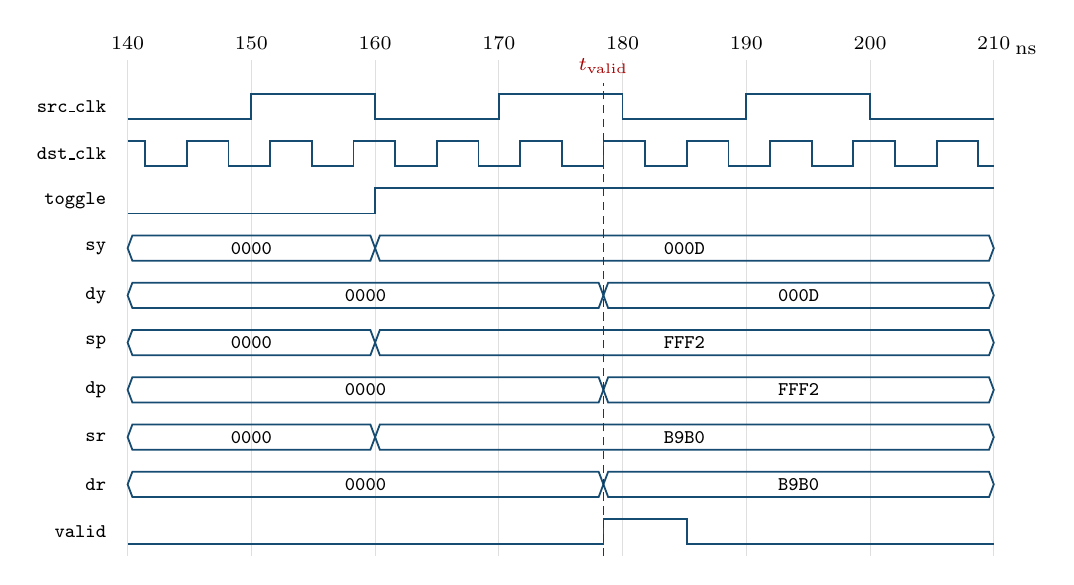
\begin{tikzpicture}[x=1cm,y=1cm,font=\scriptsize]
\tikzset{trace/.style={draw=TemplateBlue,line width=0.65pt}}
\draw[gray!25] (0.00000,-5.550) -- (0.00000,0.75);
\node[anchor=south] at (0.00000,0.76) {140};
\draw[gray!25] (1.57143,-5.550) -- (1.57143,0.75);
\node[anchor=south] at (1.57143,0.76) {150};
\draw[gray!25] (3.14286,-5.550) -- (3.14286,0.75);
\node[anchor=south] at (3.14286,0.76) {160};
\draw[gray!25] (4.71429,-5.550) -- (4.71429,0.75);
\node[anchor=south] at (4.71429,0.76) {170};
\draw[gray!25] (6.28571,-5.550) -- (6.28571,0.75);
\node[anchor=south] at (6.28571,0.76) {180};
\draw[gray!25] (7.85714,-5.550) -- (7.85714,0.75);
\node[anchor=south] at (7.85714,0.76) {190};
\draw[gray!25] (9.42857,-5.550) -- (9.42857,0.75);
\node[anchor=south] at (9.42857,0.76) {200};
\draw[gray!25] (11.00000,-5.550) -- (11.00000,0.75);
\node[anchor=south] at (11.00000,0.76) {210};
\node[anchor=west] at (11.15,0.87) {ns};
\node[anchor=east] at (-0.15,0.160) {\texttt{src\_clk}};
\draw[trace] (0.00000,0.000) -- (1.57143,0.000) -- (1.57143,0.320) -- (3.14286,0.320) -- (3.14286,0.000) -- (4.71429,0.000) -- (4.71429,0.320) -- (6.28571,0.320) -- (6.28571,0.000) -- (7.85714,0.000) -- (7.85714,0.320) -- (9.42857,0.320) -- (9.42857,0.000) -- (11.00000,0.000);
\node[anchor=east] at (-0.15,-0.440) {\texttt{dst\_clk}};
\draw[trace] (0.00000,-0.280) -- (0.22220,-0.280) -- (0.22220,-0.600) -- (0.75130,-0.600) -- (0.75130,-0.280) -- (1.28040,-0.280) -- (1.28040,-0.600) -- (1.80950,-0.600) -- (1.80950,-0.280) -- (2.33860,-0.280) -- (2.33860,-0.600) -- (2.86770,-0.600) -- (2.86770,-0.280) -- (3.39680,-0.280) -- (3.39680,-0.600) -- (3.92590,-0.600) -- (3.92590,-0.280) -- (4.45500,-0.280) -- (4.45500,-0.600) -- (4.98410,-0.600) -- (4.98410,-0.280) -- (5.51320,-0.280) -- (5.51320,-0.600) -- (6.04230,-0.600) -- (6.04230,-0.280) -- (6.57140,-0.280) -- (6.57140,-0.600) -- (7.10050,-0.600) -- (7.10050,-0.280) -- (7.62960,-0.280) -- (7.62960,-0.600) -- (8.15870,-0.600) -- (8.15870,-0.280) -- (8.68780,-0.280) -- (8.68780,-0.600) -- (9.21690,-0.600) -- (9.21690,-0.280) -- (9.74600,-0.280) -- (9.74600,-0.600) -- (10.27510,-0.600) -- (10.27510,-0.280) -- (10.80420,-0.280) -- (10.80420,-0.600) -- (11.00000,-0.600);
\node[anchor=east] at (-0.15,-1.040) {\texttt{toggle}};
\draw[trace] (0.00000,-1.200) -- (3.14286,-1.200) -- (3.14286,-0.880) -- (11.00000,-0.880);
\node[anchor=east] at (-0.15,-1.640) {\texttt{sy}};
\draw[trace] (0.00000,-1.640) -- (0.06000,-1.480) -- (3.08286,-1.480) -- (3.14286,-1.640) -- (3.08286,-1.800) -- (0.06000,-1.800) -- cycle;
\node at (1.57143,-1.640) {\texttt{0000}};
\draw[trace] (3.14286,-1.640) -- (3.20286,-1.480) -- (10.94000,-1.480) -- (11.00000,-1.640) -- (10.94000,-1.800) -- (3.20286,-1.800) -- cycle;
\node at (7.07143,-1.640) {\texttt{000D}};
\node[anchor=east] at (-0.15,-2.240) {\texttt{dy}};
\draw[trace] (0.00000,-2.240) -- (0.06000,-2.080) -- (5.98230,-2.080) -- (6.04230,-2.240) -- (5.98230,-2.400) -- (0.06000,-2.400) -- cycle;
\node at (3.02115,-2.240) {\texttt{0000}};
\draw[trace] (6.04230,-2.240) -- (6.10230,-2.080) -- (10.94000,-2.080) -- (11.00000,-2.240) -- (10.94000,-2.400) -- (6.10230,-2.400) -- cycle;
\node at (8.52115,-2.240) {\texttt{000D}};
\node[anchor=east] at (-0.15,-2.840) {\texttt{sp}};
\draw[trace] (0.00000,-2.840) -- (0.06000,-2.680) -- (3.08286,-2.680) -- (3.14286,-2.840) -- (3.08286,-3.000) -- (0.06000,-3.000) -- cycle;
\node at (1.57143,-2.840) {\texttt{0000}};
\draw[trace] (3.14286,-2.840) -- (3.20286,-2.680) -- (10.94000,-2.680) -- (11.00000,-2.840) -- (10.94000,-3.000) -- (3.20286,-3.000) -- cycle;
\node at (7.07143,-2.840) {\texttt{FFF2}};
\node[anchor=east] at (-0.15,-3.440) {\texttt{dp}};
\draw[trace] (0.00000,-3.440) -- (0.06000,-3.280) -- (5.98230,-3.280) -- (6.04230,-3.440) -- (5.98230,-3.600) -- (0.06000,-3.600) -- cycle;
\node at (3.02115,-3.440) {\texttt{0000}};
\draw[trace] (6.04230,-3.440) -- (6.10230,-3.280) -- (10.94000,-3.280) -- (11.00000,-3.440) -- (10.94000,-3.600) -- (6.10230,-3.600) -- cycle;
\node at (8.52115,-3.440) {\texttt{FFF2}};
\node[anchor=east] at (-0.15,-4.040) {\texttt{sr}};
\draw[trace] (0.00000,-4.040) -- (0.06000,-3.880) -- (3.08286,-3.880) -- (3.14286,-4.040) -- (3.08286,-4.200) -- (0.06000,-4.200) -- cycle;
\node at (1.57143,-4.040) {\texttt{0000}};
\draw[trace] (3.14286,-4.040) -- (3.20286,-3.880) -- (10.94000,-3.880) -- (11.00000,-4.040) -- (10.94000,-4.200) -- (3.20286,-4.200) -- cycle;
\node at (7.07143,-4.040) {\texttt{B9B0}};
\node[anchor=east] at (-0.15,-4.640) {\texttt{dr}};
\draw[trace] (0.00000,-4.640) -- (0.06000,-4.480) -- (5.98230,-4.480) -- (6.04230,-4.640) -- (5.98230,-4.800) -- (0.06000,-4.800) -- cycle;
\node at (3.02115,-4.640) {\texttt{0000}};
\draw[trace] (6.04230,-4.640) -- (6.10230,-4.480) -- (10.94000,-4.480) -- (11.00000,-4.640) -- (10.94000,-4.800) -- (6.10230,-4.800) -- cycle;
\node at (8.52115,-4.640) {\texttt{B9B0}};
\node[anchor=east] at (-0.15,-5.240) {\texttt{valid}};
\draw[trace] (0.00000,-5.400) -- (6.04230,-5.400) -- (6.04230,-5.080) -- (7.10050,-5.080) -- (7.10050,-5.400) -- (11.00000,-5.400);
\draw[red!65!black,densely dashed] (6.04230,-5.550) -- (6.04230,.46);
\node[anchor=south,text=red!65!black] at (6.04230,.46) {$t_{\rm valid}$};
\end{tikzpicture}

\caption{本次姿态跨域仿真的首组快照波形（总线以十六进制表示）}
\label{fig:sim-cdc}
\end{figure}

100 次更新全部通过，无重复、丢失或字段混合。该测试的前提是源数据在目的端采样期间
保持稳定，且下一次更新留有足够间隔；数字 RTL 仿真不能模拟模拟电路的亚稳态概率，
相关跨域结构和时序约束仍需单独审查。
\sourcefile{\path{../Pgl50h/tests/tb_imu_protocol.sv}；
\path{../Pgl50h/tests/tb_attitude_cdc.sv}；
\path{chapter5/references/local_20261025/attitude_cdc.vcd}}

\section{像素预处理与帧级配置验证}
\subsection{Gamma 数值参考和视频节拍}
Gamma 测试使用数学公式独立计算表项期望值：
\begin{equation}
C_{\mathrm{ref}}=\operatorname{round}\!\left[255
\left(\frac{C_{\mathrm{in}}}{255}\right)^\gamma\right],
\qquad C_{\mathrm{in}}\in\{0,\ldots,255\}.
\end{equation}
七条有效曲线与一个保留恒等档共 2048 个表项全部比较，
不以“读取 DUT 的 LUT 再与 DUT 输出比较”作为数值参考。
像素计分板进一步检查三个颜色通道以及 DE、VS 的两级寄存器延迟，
包括增强关闭时的恒等像素行为与同样的节拍延迟。

场景激励包含暗场 16、亮场 224、明暗混合 32/224、中性灰 128、
各通道变化及 111/112 分类阈值附近的输入。测试检查分类滞回、
曲线逐档变化和帧内配置稳定性，主动在帧中改变启用请求，确认不会从半帧开始换曲线。
帧统计还检查末像素是否被计入、空帧和启动阶段是否被错误发布。
本次共核对 15365 个有效像素和 60 次统计，全部通过。

另有 10 月 22 日归档的 \path{tb_adaptive_gamma_1080p}，
在 148.5 MHz、60 Hz 完整光栅下检查 2073600 个像素不插入额外周期。
全白帧亮度和为
\begin{equation}
S_{\max}=255\times1920\times1080=528768000<2^{29},
\end{equation}
归档记录与此值精确一致。该结果用于补充整帧统计容量和连续节拍证据，
不是本次重新执行的第十二项测试。

\subsection{运行时掩码、SOF 原子应用和首像素对齐}
\path{tb_pc_control} 遍历三位功能掩码的全部 8 种组合，
bit0、bit1、bit2 分别控制镜头去畸变、姿态矫正和自适应 Gamma。
测试检查串口命令校验、未完成帧超时、busy 时拒收、状态查询与连续遥测，
重点区分“接收请求”和“输入 SOF 应用请求”两个时刻。
无 SOF 时 \path{requested_mask} 可以改变，
\path{applied_mask} 必须保持原值，并保留 pending 状态。

仅在简单测试平台中同时翻转掩码和 SOF，容易遗漏真实像素寄存器带来的相位差。
因此，本次还执行 \path{tb_pc_control_frame_alignment}，
串联输入寄存、控制跨域、Gamma 和 RGB565 转换，
在 SOF 与首个 DE 同时出现等条件下比较像素与帧元数据。
25 帧测试覆盖全部掩码与 pending 命令，检查首像素使用的 Gamma 开关、
几何控制和遥测帧身份一致，未发现一帧内混用新旧配置。

\begin{table}[htbp]\centering\small
\caption{帧级一致性检查及失败含义}\label{tab:sim-frame-atomic}
\begin{tabularx}{\textwidth}{>{\raggedright\arraybackslash}p{3.2cm}YY}
\toprule
检查事件 & 自动判定条件 & 可发现的问题 \\
\midrule
命令接收后尚无 SOF & 已应用配置不变，请求保持 pending & 串口 ACK 后立即切换半帧配置 \\
SOF 与首 DE 同时到达 & 首像素与该帧掩码使用相同配置 & 控制与像素流水线相差一拍 \\
帧内修改启用请求 & 当前完整帧的曲线和开关保持稳定 & 半帧亮度突变或错误统计归属 \\
Gamma 统计跨域 & 像素数、亮度和、曲线、掩码属于同一帧 & 分别同步多位字段导致快照撕裂 \\
\bottomrule
\end{tabularx}
\end{table}

\subsection{遥测与输出格式}
\path{tb_gamma_telemetry} 使用 \texttt{COLOR=1}，
独立计算彩色像素经 Gamma 后的 RGB 和近似亮度，
比较增强前后亮度和以及先前完成帧的曲线、掩码元数据，检查统计快照跨域时的一致性。
该检查防止出现“像素总数属于上一帧，而曲线号已属于下一帧”的情况。
统计位置在几何重采样和 RGB565 量化之前，其正确性不等于最终输出图像质量已获得验证。

输出格式测试穷举全部 65536 种 RGB565 输入，检查按位扩展至 RGB888 的结果及 DE 原样转发，
并分别检查默认 23 拍与参数化 2 拍光栅延迟，以及流水线占用期间的复位。
因此，格式测试的判据是像素位值与显示节拍一致，而非仅观察屏幕是否有图像。
\sourcefile{\path{../Pgl50h/tests/tb_adaptive_gamma_stream.sv}；
\path{../Pgl50h/tests/tb_pc_control_frame_alignment.sv}；
\path{../Pgl50h/tests/tb_gamma_telemetry.sv}；
\path{../Pgl50h/tests/tb_rgb888_raster.sv}；整帧 Gamma 归档见
\path{../Pgl50h/verification/pds_pc_control_write_ram_20261022/pc_control/03_tb_adaptive_gamma_1080p.log}}

\section{逆映射与分块渲染验证}
\subsection{坐标运算模块的参考点测试}
\path{tb_pose_inverse_project_q14} 采用默认除法实现，
先加载姿态并等待 \path{pose_ready}，再输入目的像素，
检查输出有效、源坐标和映射有效标志。
零姿态检查参考点 $(944,522)$，正负 yaw 约 $30^\circ$、pitch 约 $20^\circ$
以及组合姿态用于检查轴向、符号和投影方向；超限输入检查约 $35^\circ$ 的模块限幅，
并要求视场外坐标标记为无效，不能简单复制边界像素。

上述宽角度激励属于坐标模块测试，默认系统工作范围仍为 yaw/pitch 每轴约
$\pm15^\circ$。测试中参考点的允许误差为 2--5 像素，
因此通过结果只能说明这些参考点满足既定数值容差，
不能据此声称全视场亚像素精度、极低直线度误差或 MTF50 达标。

\subsection{分块遍历、缓存和逐像素计分板}
本次对 \path{tb_pose_renderer_tiled} 设置
\texttt{WIDTH=144, HEIGHT=40, TILE\_W=128, TILE\_H=32}，
保留其默认源图像 $320\times180$ 和测试内参 $f_x=f_y=125$、$(c_x,c_y)=(160,90)$。
这是截取左上方输出区域的功能测试，不是把完整标定图像缩放到 $144\times40$。
横向与纵向均产生一个完整块和一个裁剪块，四块分别为
$128\times32$、$16\times32$、$128\times8$、$16\times8$，
可直接覆盖右侧不足块宽和底部不足块高的边界。

源图像使用由 bank、横坐标和纵坐标共同决定的合成 RGB565 图样。
测试枚举所有目的像素，建立期望颜色数组和访问标志；每笔输出写突发到达时，
逐 beat、逐像素比较颜色，并拒绝越界、重复或遗漏输出。
源数据地址和输出地址还必须属于正确的帧 bank，突发长度必须处于 1--16 beats。
参考坐标由另一个相同的逆映射模块生成，故该计分板主要独立检查
调度、缓存寻址、采样和提交链路，不构成对投影公式的独立高精度复核。

渲染开始后，测试主动改变输入姿态、源 bank、输出 bank 和镜头使能请求，
要求当前任务继续使用启动时锁存的快照；读、写命令就绪分别周期性停顿，
响应延迟以 24 拍为基础附加变化，检查等待期间命令地址、长度和写载荷保持稳定。
只有全部输出写事务收到完成响应后才允许发布结果。

\begin{table}[htbp]\centering\small
\caption{本次 $144\times40$ 分块渲染测试结果}\label{tab:sim-tiled-results}
\begin{tabularx}{\textwidth}{rr*{5}{>{\centering\arraybackslash}X}}
\toprule
\multicolumn{2}{c}{姿态（Q2048）} & 耗时/拍 & 源读命令 & 源读 beats & 有效像素 & 黑色填充 \\
\cmidrule(lr){1-2}
yaw & pitch & & & & & \\
\midrule
0 & 0 & 12644 & 91 & 403 & 5760 & 0 \\
536 & 536 & 11552 & 23 & 129 & 866 & 4894 \\
536 & $-536$ & 12589 & 87 & 393 & 5760 & 0 \\
$-536$ & 536 & 10833 & 2 & 2 & 4 & 5756 \\
$-536$ & $-536$ & 12512 & 88 & 416 & 4279 & 1481 \\
\bottomrule
\end{tabularx}
\end{table}

表~\ref{tab:sim-tiled-results} 的 $536/2048$ rad 约为 $15^\circ$。
每组姿态均完成 5760 个目的像素、80 笔输出写事务；五组共比较 28800 个输出像素，
块边界、姿态快照和最后写入提交检查全部通过。
由于测试仅覆盖左上角区域，部分姿态下大多数坐标落到源视场之外；
黑色填充计数差异反映该测试几何条件，不能用来代表整幅输出的有效视场比例。
无效像素减少了源读取量，也使本表耗时不能直接外推到完整 1080p 帧率。

最后一次测试注入错误的读 LAST，确认模块报告错误后保持 busy、禁止 done，
防止错误帧被当作完整结果发布。
\sourcefile{\path{../Pgl50h/tests/tb_pose_inverse_project_q14.sv}；
\path{../Pgl50h/tests/tb_pose_renderer_tiled.sv}；
\path{chapter5/references/local_20261025/pose_renderer_tiled.log}}

\section{异步缓存与共享 DDR 协议验证}
\subsection{异步 FIFO 的顺序、反压和复位}
\path{tb_pose_async_fifo} 同时测试三种配置：256 bit、512 深度用于接近采集缓存的规模，
37 bit、8 深度以及 8 bit、2 深度用于快速触发满空边界和指针回绕。
各实例采用不同写读时钟，并插入随机停顿，由队列计分板核对读出顺序。
检查内容包含满时不写、空时不读、反压时输出保持、信用计数不高估可用空间，
以及 FIFO 非空时复位能够清除原有事务。

三组实例分别完成 12260/11488、15108/15096、3526/3522 次写/读，
所有检查通过。写读总数不同与测试中的非空复位及结束时残留有关，
不能直接把两者差值解释为丢失数据；无复位区间内的数据顺序由计分板逐项约束。

\subsection{DDR 仲裁与实际完成事件}
\path{tb_pose_ddr_arbiter} 设置 \texttt{STREAM=1}，
检查共享写载荷路径。采集写与渲染写、显示读与渲染读同时竞争时，
测试检查优先级、唯一事务归属和返回路由。行为模型独立停顿地址接收与数据传输，
插入最长 31 拍的延迟，避免使用固定计时器的错误完成逻辑侥幸通过。

工程所用 DDR 用户接口具有 AW/AR、WREADY、RVALID 和 LAST 等信号，
但没有完整 AXI4 的 WVALID、RREADY 与 B 响应通道；写侧 LAST 来自控制器。
因此，本章按该 IP 的接口约定判断有效数据拍，不套用完整 AXI4 的五通道握手规则。
每次有效写拍都比较载荷和 beat 序号，最后拍检查 LAST 与长度一致，
并要求完成信号只返回给该事务所属客户端。

图~\ref{fig:sim-ddr} 为本次仿真的三拍采集写片段，
\path{axi_awlen}=\texttt{2} 表示总计三个 beats。
755 ns 的上升沿接受地址，之后三个写数据拍分别在 815、935、1075 ns 被接受；
中间出现长时间 WREADY 停顿，\path{write_beat_index} 只能在真实数据拍后推进。
\path{cap_w_done} 于最后拍对应时刻产生，\path{protocol_error} 保持为零。
这组波形说明“地址已接受”与“最后数据已提交”是不同事件，
输出帧的发布不能由地址握手或估计延迟替代。

\begin{figure}[htbp]\centering
% Generated from actual VCD by references/make_waveforms.py.
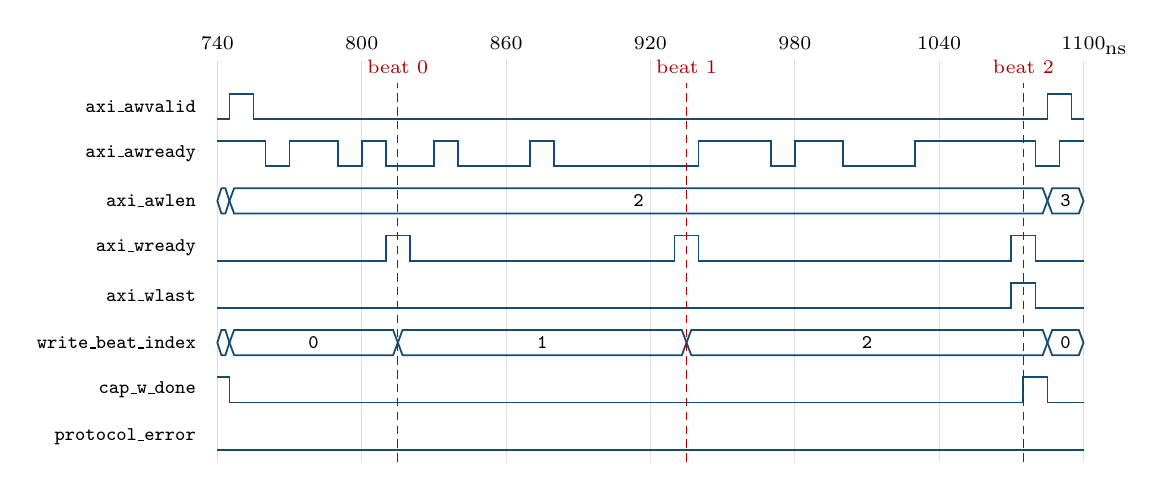
\begin{tikzpicture}[x=1cm,y=1cm,font=\scriptsize]
\tikzset{trace/.style={draw=TemplateBlue,line width=0.65pt}}
\draw[gray!25] (0.00000,-4.350) -- (0.00000,0.75);
\node[anchor=south] at (0.00000,0.76) {740};
\draw[gray!25] (1.83333,-4.350) -- (1.83333,0.75);
\node[anchor=south] at (1.83333,0.76) {800};
\draw[gray!25] (3.66667,-4.350) -- (3.66667,0.75);
\node[anchor=south] at (3.66667,0.76) {860};
\draw[gray!25] (5.50000,-4.350) -- (5.50000,0.75);
\node[anchor=south] at (5.50000,0.76) {920};
\draw[gray!25] (7.33333,-4.350) -- (7.33333,0.75);
\node[anchor=south] at (7.33333,0.76) {980};
\draw[gray!25] (9.16667,-4.350) -- (9.16667,0.75);
\node[anchor=south] at (9.16667,0.76) {1040};
\draw[gray!25] (11.00000,-4.350) -- (11.00000,0.75);
\node[anchor=south] at (11.00000,0.76) {1100};
\node[anchor=west] at (11.15,0.87) {ns};
\node[anchor=east] at (-0.15,0.160) {\texttt{axi\_awvalid}};
\draw[trace] (0.00000,0.000) -- (0.15278,0.000) -- (0.15278,0.320) -- (0.45833,0.320) -- (0.45833,0.000) -- (10.54167,0.000) -- (10.54167,0.320) -- (10.84722,0.320) -- (10.84722,0.000) -- (11.00000,0.000);
\node[anchor=east] at (-0.15,-0.440) {\texttt{axi\_awready}};
\draw[trace] (0.00000,-0.280) -- (0.61111,-0.280) -- (0.61111,-0.600) -- (0.91667,-0.600) -- (0.91667,-0.280) -- (1.52778,-0.280) -- (1.52778,-0.600) -- (1.83333,-0.600) -- (1.83333,-0.280) -- (2.13889,-0.280) -- (2.13889,-0.600) -- (2.75000,-0.600) -- (2.75000,-0.280) -- (3.05556,-0.280) -- (3.05556,-0.600) -- (3.97222,-0.600) -- (3.97222,-0.280) -- (4.27778,-0.280) -- (4.27778,-0.600) -- (6.11111,-0.600) -- (6.11111,-0.280) -- (7.02778,-0.280) -- (7.02778,-0.600) -- (7.33333,-0.600) -- (7.33333,-0.280) -- (7.94444,-0.280) -- (7.94444,-0.600) -- (8.86111,-0.600) -- (8.86111,-0.280) -- (10.38889,-0.280) -- (10.38889,-0.600) -- (10.69444,-0.600) -- (10.69444,-0.280) -- (11.00000,-0.280);
\node[anchor=east] at (-0.15,-1.040) {\texttt{axi\_awlen}};
\draw[trace] (0.00000,-1.040) -- (0.05093,-0.880) -- (0.10185,-0.880) -- (0.15278,-1.040) -- (0.10185,-1.200) -- (0.05093,-1.200) -- cycle;
\draw[trace] (0.15278,-1.040) -- (0.21278,-0.880) -- (10.48167,-0.880) -- (10.54167,-1.040) -- (10.48167,-1.200) -- (0.21278,-1.200) -- cycle;
\node at (5.34722,-1.040) {\texttt{2}};
\draw[trace] (10.54167,-1.040) -- (10.60167,-0.880) -- (10.94000,-0.880) -- (11.00000,-1.040) -- (10.94000,-1.200) -- (10.60167,-1.200) -- cycle;
\node at (10.77083,-1.040) {\texttt{3}};
\node[anchor=east] at (-0.15,-1.640) {\texttt{axi\_wready}};
\draw[trace] (0.00000,-1.800) -- (2.13889,-1.800) -- (2.13889,-1.480) -- (2.44444,-1.480) -- (2.44444,-1.800) -- (5.80556,-1.800) -- (5.80556,-1.480) -- (6.11111,-1.480) -- (6.11111,-1.800) -- (10.08333,-1.800) -- (10.08333,-1.480) -- (10.38889,-1.480) -- (10.38889,-1.800) -- (11.00000,-1.800);
\node[anchor=east] at (-0.15,-2.240) {\texttt{axi\_wlast}};
\draw[trace] (0.00000,-2.400) -- (10.08333,-2.400) -- (10.08333,-2.080) -- (10.38889,-2.080) -- (10.38889,-2.400) -- (11.00000,-2.400);
\node[anchor=east] at (-0.15,-2.840) {\texttt{write\_beat\_index}};
\draw[trace] (0.00000,-2.840) -- (0.05093,-2.680) -- (0.10185,-2.680) -- (0.15278,-2.840) -- (0.10185,-3.000) -- (0.05093,-3.000) -- cycle;
\draw[trace] (0.15278,-2.840) -- (0.21278,-2.680) -- (2.23167,-2.680) -- (2.29167,-2.840) -- (2.23167,-3.000) -- (0.21278,-3.000) -- cycle;
\node at (1.22222,-2.840) {\texttt{0}};
\draw[trace] (2.29167,-2.840) -- (2.35167,-2.680) -- (5.89833,-2.680) -- (5.95833,-2.840) -- (5.89833,-3.000) -- (2.35167,-3.000) -- cycle;
\node at (4.12500,-2.840) {\texttt{1}};
\draw[trace] (5.95833,-2.840) -- (6.01833,-2.680) -- (10.48167,-2.680) -- (10.54167,-2.840) -- (10.48167,-3.000) -- (6.01833,-3.000) -- cycle;
\node at (8.25000,-2.840) {\texttt{2}};
\draw[trace] (10.54167,-2.840) -- (10.60167,-2.680) -- (10.94000,-2.680) -- (11.00000,-2.840) -- (10.94000,-3.000) -- (10.60167,-3.000) -- cycle;
\node at (10.77083,-2.840) {\texttt{0}};
\node[anchor=east] at (-0.15,-3.440) {\texttt{cap\_w\_done}};
\draw[trace] (0.00000,-3.280) -- (0.15278,-3.280) -- (0.15278,-3.600) -- (10.23611,-3.600) -- (10.23611,-3.280) -- (10.54167,-3.280) -- (10.54167,-3.600) -- (11.00000,-3.600);
\node[anchor=east] at (-0.15,-4.040) {\texttt{protocol\_error}};
\draw[trace] (0.00000,-4.200) -- (11.00000,-4.200);
\draw[red!65!black,densely dashed] (2.29167,-4.350) -- (2.29167,.46);
\node[anchor=south,text=red!65!black] at (2.29167,.46) {beat 0};
\draw[red!65!black,densely dashed] (5.95833,-4.350) -- (5.95833,.46);
\node[anchor=south,text=red!65!black] at (5.95833,.46) {beat 1};
\draw[red!65!black,densely dashed] (10.23611,-4.350) -- (10.23611,.46);
\node[anchor=south,text=red!65!black] at (10.23611,.46) {beat 2};
\end{tikzpicture}

\caption{三拍采集写事务在 DDR 反压下的完成时序（标线对应数据接受时钟沿）}
\label{fig:sim-ddr}
\end{figure}

本次正常事务共核对 160 笔写、760 个写 beats，以及 128 笔读、488 个读 beats。
此外，平台专门检查地址与首拍同周期的边界条件，并注入异常 LAST 和响应 ID，
要求错误被识别且完成事件不被错误路由。
上述协议验证通过后，仍需使用厂商模型检查真实控制器的突发边界与延迟分布。
\sourcefile{\path{../Pgl50h/tests/tb_pose_async_fifo.sv}；
\path{../Pgl50h/tests/tb_pose_ddr_arbiter.sv}；
\path{chapter5/references/local_20261025/pose_ddr_arbiter.vcd}}

\section{厂商模型与整帧并发归档复核}
\subsection{实际 DDR 控制器的突发边界测试}
10 月 10 日的 \path{tb_pose_vendor_ddr} 归档连接生成的
\path{DDR3_50H} 控制器、PHY 及两颗 Micron x16 DDR3 仿真模型。
测试覆盖 1--16 beats 的合法突发，并把起点放在 512/1024 个 32 bit 地址单位边界之前，
其中 1024 个地址单位对应 4 KiB。
为避免写入和读回共享相同的回绕错误，测试采用“突发写、单 beat 读回”和
“单 beat 写、突发读回”的非对称参考；另外检查 16 行、
行步长 960 个地址单位的源图像区域，等价于每行 1920 个 RGB565 像素。

归档共比较 472 个写 beats、608 个读 beats，数据和 LAST 位置检查通过。
100 MHz 用户时钟下，AR 接受到首个 RVALID 为 27--29 拍，
8-beat、16-beat 读到末拍分别为 34--41、42--49 拍，
AW 首次有效至最后 WREADY 的最大观测值为 245 拍。
模型中的跨行和成组刷新引入额外间隙，说明功能测试使用的 24 拍基础延迟
不能被当成真实 DDR 最坏访问延迟。

该归档未发现仿真 Error、Fatal 或 Micron 时序违规，存在 33 条与旧版生成 IP
端口、位宽和工具设置有关的 Warning。测试为短事务序列，
没有同时施加全速采集、渲染和显示负载，故不能单独证明整帧吞吐。
\sourcefile{\path{../Pgl50h/verification/pose_tiled_20261010/vendor_ddr_boundary_latency/README.md}；
同目录 \path{sim.log} 与 \path{source_identity.json}}

\subsection{完整 1080p 并发链路}
10 月 22 日归档的 \path{tb_fram_buf_pose_tiled} 在 ModelSim SE-64 10.6e 下运行，
输入为 $1920\times1080$ 完整光栅，共施加 28 个输入帧，启用预处理、运行时控制
与共享数据通道。DDR 行为模型设置基础延迟 32 拍、25\% 数据气泡，
并每 780 拍插入 35 拍刷新暂停；这与上一节厂商模型的实际短事务 trace 是两组不同条件。

\begin{table}[htbp]\centering\small
\caption{10 月 22 日整帧并发归档的功能观测}\label{tab:sim-full-archive}
\begin{tabularx}{\textwidth}{>{\raggedright\arraybackslash}p{4.2cm}Y}
\toprule
观测项 & 归档结果与解释 \\
\midrule
显示数据计分板 & 比较 51840000 个显示像素，检查帧身份及输出内容 \\
姿态与控制激励 & 11 组姿态激励及全部 8 种功能掩码；未穷举两者的笛卡尔积 \\
新结果发布 & 发布 13 帧；约 30.000030 fps，区别于 60 Hz 显示光栅 \\
最慢渲染与发布间隔 & 3314614 拍与 3333330 拍，按 100 MHz DDR 用户时钟计 \\
采集 FIFO 峰值 & 15/512，用于检查该场景下的缓冲压力 \\
日志状态 & 0 Error、4 Warning；警告涉及 Gamma 统计元数据未连接 \\
\bottomrule
\end{tabularx}
\end{table}

归档中的源帧编号会跳过部分输入帧，发布结果序列包含
1、2、5、7、\ldots、25；因此，通过判据是按系统策略发布完整且身份一致的新结果，
并非要求每个 60 Hz 输入帧都完成矫正。
该测试没有经真实 UART 注入全部控制流，也没有连接厂商 DDR PHY 模型。
后续源码已有修改，10 月 25 日复跑的小区域测试只能增加当前功能证据，
不能将上述 1080p 吞吐结果认定为当前全部源码的重测结论。
版本对应、帧率预算和性能余量进一步见第~\ref{chap:verification}~章。
\sourcefile{\path{../Pgl50h/verification/pds_pc_control_write_ram_20261022/simulation/result.log}；
同目录 \path{source_identity.json} 与 \path{../input_snapshot/}}

\section{复现方法与待补充验证}
在本报告根目录可执行
\begin{quote}\small\ttfamily
python3 chapter5/references/run\_simulations.py\\
python3 chapter5/references/make\_waveforms.py
\end{quote}
第一条命令运行表~\ref{tab:sim-matrix} 的 11 项测试并生成日志与清单，
第二条从 VCD 提取图~\ref{fig:sim-cdc}、图~\ref{fig:sim-ddr} 的真实信号跳变，
生成可随正文编译的 TikZ 波形。工程位置改变时，可通过
\texttt{--project} 指定路径；独立保留新结果可使用 \texttt{--output}。
波形生成脚本默认读取本章归档目录。

现有结果支持所选激励下的串口解析、跨域一致性、像素节拍、帧配置原子应用、
分块遍历和 DDR 完成语义。后续应在同一源码快照上重跑完整 1080p 并发压力测试，
补充复位与异常恢复、长时间多姿态切换及厂商 DDR 并发负载，
并将仿真快照与最终约束、实现报告和位流对应。
板级连续运行、端到端延迟和图卡清晰度仍须分别测量；
MTF50/SFR、直线度和边缘拉伸/断裂的定量判据与记录模板见第~\ref{chap:performance}~章。

\chapter{FPGA 实时性能与资源效率}
\label{chap:verification}

本章围绕两个问题评价 FPGA 实现：一是能否在持续视频输入与显示的同时，
按期完成完整矫正帧；二是为达到这一吞吐，消耗了多少计算、存储与互连资源。
分析采用原始 RTL 仿真日志、PDS 综合和布局布线报告，以及
\path{chapter6/references/} 中的性能说明与审计记录。
其中，1080p 完整链路仿真给出了约 30 fps 的新结果发布率，
最慢观测渲染时间为 33.14614 ms；128$\times$32 分块实现则将物理 DRM
占用从历史实现的 122 个位置降至 104 个。
这两项结果分别反映已测试条件下的处理能力和存储效率，其适用版本与测量条件如下。

\section{分析配置与数据来源}
\subsection{工作配置及评价指标}
系统基于紫光同创 PGL50H-FBG484-6 FPGA。默认数据通路接收
$1920\times1080$ RGB888 视频，依次执行帧自适应 Gamma、
RGB565 量化、DDR 源帧存储、姿态与镜头畸变联合逆投影、最近邻重采样和结果写回，
再将 RGB565 展开为 RGB888 输出。输入与输出均使用 148.5 MHz 像素时钟和
60 Hz 扫描时序，矫正器的目标是每秒生成 30 个来自不同源帧的完整结果。

\begin{table}[htbp]
\centering\small
\caption{实时性能分析采用的默认配置}\label{tab:rt-config}
\begin{tabularx}{\textwidth}{p{4.4cm}Y}
\toprule
配置项 & 参数及含义 \\
\midrule
有效图像与总光栅 & $1920\times1080$；$2200\times1125$ \\
像素时钟与扫描频率 & 148.5 MHz；60 Hz \\
DDR 用户接口与渲染时钟 & 256 bit；100 MHz，每 beat 为 32 bytes \\
DDR 像素格式 & RGB565，每 beat 承载 16 个像素 \\
输出分块与片内块槽 & $128\times32$；两个块槽交替使用 \\
单槽源区域缓存 & $2048\times256$ bit，即 64 KiB \\
片外帧槽 & 两个源帧槽、两个结果帧槽 \\
几何计算与采样 & 逐像素定点逆投影；最近邻 \\
姿态配置 & yaw、pitch 各约 $\pm15^\circ$；roll 未参与变换 \\
结果交接 & 最后一笔写数据传输完成后提交，在显示帧边界切换 \\
\bottomrule
\end{tabularx}
\end{table}

本章区分扫描频率、新结果帧率、单帧渲染时间和端到端延迟。
扫描频率描述接口发送图像的节拍；新结果帧率描述不同源帧的处理产出；
渲染时间描述矫正器占用一帧任务的时间；端到端延迟还包含采集、调度与显示等待。
资源效率则分别用综合逻辑用量、最终物理占用、逻辑缓存容量和版本间变化评价。

\subsection{报告版本与证据边界}
\path{../Pgl50h/prj_tasks/} 中的报告头部标明 PDS2025.2 build 211867，
生成日期为 2026 年 10 月 21 日，其综合用量为 17,294 LUT、25,891 FF、
121 个 DRM18K 等效容量。它们属于较早的高存储占用实现，
不能作为 128$\times$32 默认版本的资源表。
表~\ref{tab:rt-evidence} 将本章使用的数据按生成日期分开。

\begin{table}[htbp]
\centering\small
\caption{性能与资源数据的版本划分}\label{tab:rt-evidence}
\begin{tabularx}{\textwidth}{p{2.1cm}>{\raggedright\arraybackslash}p{3.2cm}Y}
\toprule
证据日期 & 来源与工具 & 本章用途 \\
\midrule
2026-10-21 & 工程 \path{prj_tasks/}；PDS2025.2 & 直接读取综合、物理资源与双角时序，作为早期实现对照。\\
2026-10-22 & 完整链路仿真及配套实现归档；PDS2025.2 & 分析 $128\times32$ 的新帧率、渲染耗时、FIFO 峰值及共享写缓冲收益。\\
2026-10-24 & 本章参考说明与数值审计；PDS2025.2 & 引用复核版本的资源和时序结果，独立于 10 月 22 日的吞吐数据。\\
2026-10-25 & 本章 JSON 审计；PDS2022.2-SP3 & 说明跨工具重编译的时序失败，以及未采用修复候选的验证状态。\\
\bottomrule
\end{tabularx}
\end{table}

10 月 25 日审计将 10 月 22 日完整 1080p 测试明确标记为历史结果，
并列出了后续变化的帧缓存、渲染器、FIFO 与测试文件。
因此，30.000030 fps 是对应归档快照的结果，尚不能直接写成后续源码的重新测试值。
审计还记录了用户反馈的仓库版本板测状态，但没有核验实际烧录位流哈希，
也没有提供板级帧率或端到端延迟数值；本章据此保留功能反馈与定量测量之间的区别。
\begingroup\interlinepenalty=10000
\sourcefile{\path{chapter6/references/} 下的《02\_实时性能与资源效率.md》；
\path{chapter6/references/realtime_resource_audit_20261025.json}；
\path{../Pgl50h/prj_tasks/syn_1/synthesize/hdmi_ddr3_top.snr}}
\endgroup

\section{实时处理预算与流水重叠}
\subsection{帧率目标与单帧预算}
一帧有效图像包含
\begin{equation}
N=1920\times1080=2,073,600\ \text{pixels}.
\end{equation}
输入和显示扫描频率为
\begin{equation}
f_{\rm scan}=\frac{148.5\times10^6}{2200\times1125}
=60\ \text{Hz},\qquad T_{\rm scan}=16.66667\ \text{ms}.
\end{equation}
在此扫描时序下，有效输入像素平均速率为 124.416 Mpixel/s。
30 fps 矫正目标对应的有效处理需求与 100 MHz 域单帧预算为
\begin{align}
P_{30}&=N\times30=62.208\ \text{Mpixel/s},\\
C_{30}&=\frac{100\times10^6}{30}=3,333,333.33\ \text{cycles},\qquad
T_{30}=33.333333\ \text{ms}.
\end{align}

100 MHz 下每拍完成一个像素的单流水线，理想吞吐上限为 100 Mpixel/s，
折合完整 1080p 图像约 48.23 fps。因而默认单像素通路需要依靠流水重叠达到
30 fps；若要求完整 1080p60，即使忽略全部调度与访存开销，
100 MHz、每拍一个像素的输出通路也不足以满足 124.416 Mpixel/s 的需求。
60 Hz HDMI 可以重复显示同一完整结果帧，其连续输出并不增加矫正器的新帧产出。

\subsection{块内流水与块间并行}
$128\times32$ 分块每块最多 4096 个输出像素，一帧共有
\begin{equation}
N_{\rm tile}=\left\lceil\frac{1920}{128}\right\rceil
\left\lceil\frac{1080}{32}\right\rceil=15\times34=510\ \text{blocks}.
\end{equation}
末排高度为 24，按实际有效高度处理。每块逐像素生成逆投影坐标，
再按源包围矩形预取数据，随后采样并写回；块内像素计算使用流水线，
两个块槽则使相邻块的不同阶段重叠。

\begin{figure}[htbp]
\centering
\begin{tikzpicture}[x=1cm,y=1cm,font=\small,
  phase/.style={draw=TemplateBlue,rounded corners=2pt,minimum height=0.65cm,
    text width=3.1cm,align=center}]
\draw[-{Latex}] (1.7,0.55)--(12.9,0.55) node[above left]{处理推进};
\node[left] at (1.6,0) {块 $k$};
\node[left] at (1.6,-0.9) {块 $k+1$};
\node[left] at (1.6,-1.8) {块 $k+2$};
\node[phase,fill=TemplateBlue!8] at (3.5,0) {投影与源区域预取};
\node[phase,fill=TemplateBlue!22] at (7.0,0) {采样与结果写回};
\node[phase,fill=TemplateBlue!8] at (7.0,-0.9) {投影与源区域预取};
\node[phase,fill=TemplateBlue!22] at (10.5,-0.9) {采样与结果写回};
\node[phase,fill=TemplateBlue!8] at (10.5,-1.8) {投影与源区域预取};
\end{tikzpicture}
\caption{双块槽的阶段重叠示意。图中长度不表示实测时间；源读取与写回仍共享 DDR 服务能力。}
\label{fig:rt-overlap}
\end{figure}

若将块的投影及源加载耗时记作 $C_{\rm front}$，采样及结果写回耗时记作
$C_{\rm back}$，在资源互不争用的理想条件下，块间启动间隔可接近
$\max(C_{\rm front},C_{\rm back})$，而非两者之和。
实际系统中读写竞争、源矩形大小、块槽释放和流水排空会延长间隔，
因此图~\ref{fig:rt-overlap} 描述的是可重叠关系，不能用理想阶段时间替代整帧测量。

帧级并行进一步使采集下一幅源图、渲染已提交源帧和显示已完成结果同时进行。
两个源帧槽保护正在渲染的图像，两个结果帧槽隔离显示与写回。
渲染器只有在最后一笔有效写传输完成后才提交结果，显示侧在帧边界完成交接。
这使重复显示和输入跳帧成为吞吐调节方式，同时保证正在显示的图像不会被局部覆盖。
\begingroup\interlinepenalty=10000
\sourcefile{\path{../Pgl50h/src/video/pose/fram_buf_pose.v}；
\path{../Pgl50h/src/video/pose/pose_renderer_tiled.v}}
\endgroup

\section{完整链路吞吐与时间余量}
\subsection{仿真条件及观测结果}
10 月 22 日归档仿真使用 ModelSim SE-64 10.6e，实例化实际帧缓存、
异步 FIFO、渲染器与仲裁器，同时运行 Gamma、RGB565 转换、采集和显示。
DDR 行为模型设置 32 拍命令延迟、25\% 随机数据停顿、
读写共享每拍最多一个 256 bit 数据 beat，并每 780 拍暂停 35 拍模拟刷新。
该模型用于施加可重复的访存压力，未包含厂商 DDR PHY 和物理 UART。

\begin{table}[htbp]
\centering\small
\caption{10 月 22 日完整 1080p 并发 RTL 仿真结果}\label{tab:simulation}
\begin{tabularx}{\textwidth}{p{5.6cm}Y}
\toprule
指标 & 观测结果 \\
\midrule
输入帧 / 不同源帧结果发布数 & 28 / 13 \\
稳态新结果发布率 & 30.000030 fps \\
相邻新结果发布间隔 & 全部为 3,333,330 拍，即 33.33330 ms \\
最慢单帧渲染 & 3,314,614 拍，即 33.14614 ms \\
13 次渲染的最小值 / 平均值 & 28.70689 ms / 31.75641 ms \\
采集 FIFO 峰值 & 15/512 个 256 bit 字，即 480 bytes \\
显示像素比较次数 & 51,840,000 \\
并行与竞争记录 & 重叠 20,080,265 拍；共享通道竞争计数 396,039 \\
测试覆盖 & 11 组姿态激励、全部 8 种控制掩码 \\
日志结果 & PASS，0 errors，4 warnings \\
\bottomrule
\end{tabularx}
\end{table}

新帧率按首末完整新结果发布时刻计算。设发布数为 $M$、对应 100 MHz 计数为
$C_1$ 与 $C_M$，则
\begin{equation}
f_{\rm new}=\frac{(M-1)f_{\rm DDR}}{C_M-C_1}
=\frac{12\times100\times10^6}{45,000,053-5,000,093}
=30.000030\ \text{fps}.
\end{equation}
该值略高于 30 来自仿真时钟离散，实际意义为达到约 30 fps 的发布节拍。
28 个输入帧与 13 个结果包含启动、稳态与排空阶段，不能用两者直接相除定义稳态丢帧率。
日志中的源帧编号也显示系统选择部分源帧处理，显示端按 60 Hz 时序重复读出完整结果。

表中最小值与平均值由 13 条 \texttt{RENDER} 记录重新统计，包含启动和不同控制状态，
只说明该次运行的样本分布。姿态掩码与功能掩码覆盖并不等于两者所有组合均完成验证；
部分姿态激励下几何功能处于关闭状态。四条 warning 均与测试平台 Gamma
统计元数据端口连接有关，因此本次像素检查也不能代替完整遥测链路的验证。
\begingroup\interlinepenalty=10000
\sourcefile{\path{../Pgl50h/verification/pds_pc_control_write_ram_20261022/simulation/result.log}}
\endgroup

\subsection{整帧效率与裕量解释}
相对 30 fps 的单帧预算，最慢观测渲染的时间余量为
\begin{align}
\Delta C&=C_{30}-3,314,614=18,719.33\ \text{cycles},\\
\Delta T&=T_{30}-33.14614=0.187193\ \text{ms},\\
\eta_{\rm margin}&=\frac{\Delta T}{T_{30}}\times100\%=0.56158\%.
\end{align}
该帧平均每个输出像素消耗的周期数及有效吞吐为
\begin{equation}
c_{\rm pixel}=\frac{3,314,614}{2,073,600}=1.59848,
\qquad
P_{\rm observed}=\frac{2,073,600}{33.14614\times10^{-3}}
\approx62.5593\ \text{Mpixel/s}.
\end{equation}
这一整帧指标已经包含投影、源读取、采样、写回与等待，
不能将其中多出的 0.59848 拍/像素全部归因于 DDR 停顿。
相对单像素每拍的 100 Mpixel/s 理想上限，观测有效吞吐约为 62.56\%；
它反映整个调度与数据通路的工作效率，不是算术单元利用率。

0.56\% 的帧预算余量说明测试已达到目标，但对附加等待较敏感。
例如，增加 20,000 个不能被重叠隐藏的 100 MHz 周期将增加 0.2 ms，
足以耗尽这一余量。若结果错过显示帧边界，新图像可能推迟到下一次扫描交接，
从而使输出更新时间产生离散跳变。因此，平均帧率之外，还需要检查最大发布间隔、
最大渲染时间和显示欠载事件，不能仅凭平均吞吐判定所有场景都能按期完成。

FIFO 峰值 15/512 对应深度占用 2.93\%，说明已覆盖负载下采集侧缓冲充足。
但它只约束该次仿真的队列水位，不能推出真实 DDR 的最长无服务时间，
也不能推出渲染阶段具有相同幅度的时间余量。已有结果是有限姿态和特定压力模型下的
观测最大值，尚未构成全部姿态、全部存储调度下的最坏执行时间证明。

\section{处理延迟与显示响应}
\subsection{端到端延迟的事件定义}
本系统先提交完整源帧，再渲染并交接完整结果，因而单帧渲染时间只是总延迟的一部分。
以同一被接受源帧的输入 SOF，到其对应结果首个有效输出像素为起止事件，定义
\begin{equation}
T_{\rm e2e}=T_{\rm capture}+T_{\rm queue}+T_{\rm render}
+T_{\rm handoff}+T_{\rm active}.
\label{eq:rt-latency}
\end{equation}

\begin{table}[htbp]
\centering\small
\caption{端到端延迟分项及其统计事件}\label{tab:rt-latency}
\begin{tabularx}{\textwidth}{p{2.5cm}Y}
\toprule
分项 & 起止事件与影响因素 \\
\midrule
$T_{\rm capture}$ & 接受源帧 SOF 至该帧末笔采集写完成；包括整幅有效图像到达与输入侧排空。\\
$T_{\rm queue}$ & 源帧提交至渲染启动；受渲染器、帧槽及结果发布状态影响。\\
$T_{\rm render}$ & 渲染启动至末笔结果写完成；归档观测最大值为 33.14614 ms。\\
$T_{\rm handoff}$ & 结果提交至显示侧完成帧边界交接；包括旧读事务排空与跨域握手。\\
$T_{\rm active}$ & 完成交接至该结果首个有效像素输出；取决于消隐区及预取状态。\\
\bottomrule
\end{tabularx}
\end{table}

内部写完成表示 DDR IP 用户接口正确接受了最后一个数据 beat，
该接口没有独立写响应 B 通道；它不是对 DDR 芯片物理写入时刻的直接测量。
延迟统计应始终沿用同一接口事件定义。
若改用输入/输出 SOF 或指定位置像素作为端点，式~\eqref{eq:rt-latency}
中的扫描等待项也应相应调整，避免重复计算消隐时间。

输入寄存、Gamma 和 RGB565 转换共四拍，在 148.5 MHz 下约为 26.94 ns，
远小于毫秒级整帧缓存和渲染耗时。缩短少量输入寄存级对总响应改善有限；
减少整帧等待、提升渲染速度和避免错过显示交接窗口，才会显著影响输出响应。
在能够赶上下一次交接且没有附加阻塞的条件下，帧边界等待通常小于一个
16.67 ms 扫描周期，但现有资料不足以将该条件推广为总延迟上界。

\subsection{已有数据能够支持的延迟结论}
现有完整链路日志记录渲染和发布事件，未给出同源输入 SOF 与首个输出有效像素的
完整配对统计，故本章不将渲染耗时填作板级端到端延迟。
测量时应为接受的源帧赋予递增身份，在统一参考时钟下记录源帧接受、提交、
渲染启动、末写完成、显示槽切换及输出有效事件，匹配同一身份后计算各分项。
未被系统接受的输入帧应计入跳帧统计，不能作为延迟样本。

板级测量还应明确是否包含相机曝光、HDMI 桥、采集卡和显示设备延迟，
预热后连续记录不少于 60 s，报告样本数、平均值、P95、最大值及异常事件。
当前审计中的板级帧率与端到端延迟字段均为空，尚无可引用的定量实测值。

\section{DDR 访问效率与带宽约束}
\subsection{有效载荷与带宽预算}
一帧 RGB565 图像的有效载荷及 beat 数为
\begin{equation}
S_f=2N=4,147,200\ \text{bytes}\approx3.955\ \text{MiB},\qquad
B_f=\frac{S_f}{32}=129,600\ \text{beats}.
\end{equation}
256 bit、100 MHz 用户数据通道的理想载荷上限为
\begin{equation}
B_{\rm peak}=32\times100\times10^6=3.2\ \text{GB/s}.
\end{equation}
该值按一次数据 beat 计算，未扣除命令、读写切换、刷新、仲裁和背压，
也不表示真实板卡的持续有效带宽。以下带宽采用十进制 MB/s，存储容量采用二进制 MiB。

设每个矫正帧实际读取 $R$ 个源区域 beat，目标渲染率为 30 fps，则
\begin{table}[htbp]
\centering\small
\caption{默认路径的 DDR 有效数据预算}\label{tab:rt-bandwidth}
\begin{tabularx}{\textwidth}{p{3cm}Y>{\raggedright\arraybackslash}p{3.8cm}}
\toprule
数据流 & 预算条件 & 有效载荷带宽 \\
\midrule
源帧采集写入 & 按 60 fps 全部接受计算 & 248.832 MB/s \\
结果帧显示读取 & 每秒扫描读取 60 个完整帧 & 248.832 MB/s \\
矫正结果写回 & 每秒写回 30 个完整帧 & 124.416 MB/s \\
渲染源区域读取 & 每帧读取 $R$ beats & $0.000960R$ MB/s \\
合计 & 前三项预算加姿态相关读取 & $622.080+0.000960R$ MB/s \\
\bottomrule
\end{tabularx}
\end{table}

若仅作理想示例，假设每个源像素每帧恰好读取一次，则 $R=B_f$，
总有效载荷为 746.496 MB/s，约占接口峰值的 23.33\%。
这一比例不能解释为实测 DDR 利用率：当前分块加载可能重复读取相邻源区域，
无效块又可能不读源图，实际采集也可能跳过输入帧。
如果用 $\alpha=R/B_f$ 表示相对一次整帧读取的源载荷系数，则预算可写为
\begin{equation}
B_{\rm total}=622.080+124.416\alpha\quad\text{MB/s}.
\end{equation}
当前 $128\times32$ 完整系统日志未给出逐姿态的 $R$，
因此保留这一参数，而不将历史 $128\times64$ 的源读取数填入当前配置。

\subsection{分块、突发长度与命令开销}
渲染器根据实际采样坐标求源包围矩形，并沿水平方向对齐到 16 像素边界。
设有效坐标极值为 $x_{\min},x_{\max},y_{\min},y_{\max}$，则单块源数据需求为
\begin{equation}
B_s=\left(\left\lfloor\frac{x_{\max}}{16}\right\rfloor
-\left\lfloor\frac{x_{\min}}{16}\right\rfloor+1\right)
(y_{\max}-y_{\min}+1),\qquad B_s\le2048.
\end{equation}
矩形加载将不规则像素访问转换为连续 burst，代价是读取矩形内未被采样的像素、
横向对齐填充，以及相邻块重叠区域。姿态和镜头参数改变矩形的形状，
因此源读取量和处理耗时均随场景变化。

内部 burst 长度为 1～16 beat。完整 $128$ 像素输出行包含 8 beat，
最大 $128\times32$ 块包含 256 beat；按当前逐行写回组织，
全帧结果约需 $15\times1080=16,200$ 笔 8-beat 写事务。
将块高从 64 减为 32，并不直接改变每行 8 beat 的打包方式，
但使块级投影准备、容量检查和槽切换次数从 255 增至 510，
也可能增加源矩形边界的重复读取。

以不重叠命令与数据的孤立事务为例，忽略随机停顿时，32 拍命令等待与 $L$ 拍载荷
对应的效率为 $L/(32+L)$：8-beat 约为 20\%，16-beat 约为 33.33\%。
这只是说明短突发对等待敏感的简化模型；实际完整系统存在多阶段重叠，
不能把该比例直接乘以接口峰值作为实测持续带宽。
模型中的 25\% 数据停顿与刷新还会进一步减少可服务周期，
两种停顿是否重合也会影响结果，故不能将各比例简单相加得到总损失。

\subsection{带宽充足与按期完成的区别}
显示端必须按有效像素节拍持续供数，采集端必须及时接收输入；
两者对服务间隔敏感，而渲染端还要在 33.33 ms 内完成一帧。
即使平均数据量低于 3.2 GB/s，集中出现的命令等待、刷新或仲裁也可能造成
FIFO 欠载或错过发布窗口。归档中的共享竞争与刷新暂停计数证明确实存在等待，
但这些计数会与其他流水活动重叠，不能全部线性累加为单帧延迟。

因此，DDR 效率应结合有效 beat 数、命令数、平均 burst 长度、各客户端等待时间、
FIFO 最高/最低水位以及帧完成期限评价。当前已有完整链路压力测试与采集 FIFO 峰值，
能够支持已覆盖条件下的吞吐结论；板级持续带宽及各姿态访问放大仍需对应事件计数。

\section{资源占用与存储组织效率}
\subsection{综合逻辑与最终物理资源}
表~\ref{tab:rt-synthesis} 列出三个 PDS2025.2 版本的综合结果。
前两列直接读取原始 SNR，10 月 24 日列采用本章参考资料中的数值。
APM 是 PDS 的 DSP 类算术资源名称，DRM18K 等效量按存储块容量折算；
分布式 RAM LUT 已包含在总 LUT 中，不能再次相加。

\begin{table}[htbp]
\centering\small
\caption{不同版本的综合资源用量}\label{tab:rt-synthesis}
\begin{tabularx}{\textwidth}{Yrrrr}
\toprule
资源 & 10 月 21 日 & 10 月 22 日 & 10 月 24 日 & 器件容量 \\
\midrule
LUT & 17,294 & 14,571 & 14,565 & 42,800 \\
FF & 25,891 & 15,006 & 15,010 & 64,200 \\
APM & 45 & 45 & 45 & 84 \\
DRM18K 等效量 & 121 & 103 & 103 & 134 \\
分布式 RAM LUT & 82 & 594 & 594 & 17,000 \\
锁存器 & 0 & 0 & 0 & --- \\
\bottomrule
\end{tabularx}
\end{table}

物理报告进一步包含常量、旁路、实际存储位置以及映射后的寄存器组织。
表~\ref{tab:rt-physical} 的 FF 均使用 CLMA 与 CLMS 内 FF 之和，不包含 I/O 寄存器。
10 月 21 日的 LUT 为 $11,914+7,438=19,352$，
FF 为 $15,911+9,845=25,756$；10 月 22 日对应为
$10,181+6,697=16,878$ 和 $9,312+5,559=14,871$。

\begin{table}[htbp]
\centering\small
\caption{布局布线后的物理资源及 10 月 24 日版本余量}\label{tab:rt-physical}
\begin{tabularx}{\textwidth}{Yrrrrr}
\toprule
资源 & 10 月 21 日 & 10 月 22 日 & 10 月 24 日 & 占用率 & 剩余 \\
\midrule
LUT & 19,352 & 16,878 & 16,897 & 39.48\% & 25,903 \\
CLM FF & 25,756 & 14,871 & 14,875 & 23.17\% & 49,325 \\
APM & 45 & 45 & 45 & 53.57\% & 39 \\
DRM 位置 & 122 & 104 & 104 & 77.61\% & 30 \\
\bottomrule
\end{tabularx}
\end{table}
占用率与剩余量对应 10 月 24 日列，按各类器件容量重新计算。

10 月 22 日与 24 日的 DRM 均由 102 个 DRM18K 和 2 个 DRM9K 构成。
按容量为 $102+2/2=103$ 个 DRM18K 等效量，利用率 76.87\%；
按位置则为 $102+2=104$ 个，利用率 77.61\%。
9K 模式占据物理位置，剩余容量也不能任意拼接，因此两种统计不能互换。
原始物理表常使用向上取整的整数百分比，例如 $122/134$ 显示为 92\%；
本章统一以计数重新计算为 91.04\%，避免将显示取整误认为资源变化。

10 月 24 日物理 LUT 比综合 LUT 多 2332 个，FF 则少 135 个。
这反映了映射、常量及旁路计数和寄存器统计边界的差异，
不宜将综合与物理列的差额直接解释为新增算法开销。
从主要数据资源看，DRM 是最紧张的一类，APM 次之，LUT 和 FF 相对宽裕。
此外，10 月 22 日 ROR 中 BKCL 已使用 4/4；
后续功能扩展还受专用时钟资源、布局位置和布线能力约束，不能仅按空余 LUT 推断可扩展规模。
\begingroup\interlinepenalty=10000
\sourcefile{\path{../Pgl50h/prj_tasks/pnr_1/place_route/hdmi_ddr3_top.rur}；
\path{../Pgl50h/verification/pds_pc_control_write_ram_20261022/prj_tasks/pnr_1/place_route/hdmi_ddr3_top.ror}；
\path{chapter6/references/realtime_resource_audit_20261025.json}}
\endgroup

\subsection{模块资源归因与计算开销}
层次综合报告可以定位资源集中在哪些功能。
表~\ref{tab:rt-modules} 将较早实现与共享写缓冲实现按同名模块对照；
父模块用量包含子模块，表中各行不能相加作为全设计总量。

\begin{table}[htbp]
\centering\small
\caption{10 月 21 日至 22 日的模块资源变化}\label{tab:rt-modules}
\begin{tabularx}{\textwidth}{Yrrr}
\toprule
模块与统计项 & 10 月 21 日 & 10 月 22 日 & 变化 \\
\midrule
帧缓存整体 LUT / FF & 10,157 / 19,834 & 6766 / 7574 & 逻辑与寄存器减少 \\
分块渲染器 LUT / FF & 5202 / 10,149 & 5442 / 6076 & LUT 略增，FF 减少 \\
分块渲染器 DRM 等效量 & 101.5 & 83.5 & 减少 18 \\
投影器 LUT / FF & 4454 / 5439 & 4443 / 5440 & 基本不变 \\
投影器 APM & 43 & 43 & 不变 \\
DDR 仲裁器 LUT / FF & 4202 / 4684 & 350 / 592 & 减少 3852 / 4092 \\
DDR 控制器及 PHY LUT / FF & 6074 / 5076 & 6070 / 5076 & 基本不变 \\
\bottomrule
\end{tabularx}
\end{table}

投影器使用 43/45 个全设计 APM，占 95.56\%，说明算术资源主要服务于逐像素几何计算。
而源、坐标、输出块缓存和 FIFO 主导 DRM 用量，二者对应不同优化方向。
DDR 控制器及 PHY 在 10 月 22 日占 6070 LUT、5076 FF，
约为全设计综合 LUT 的 41.66\% 和 FF 的 33.83\%；
这些是支撑视频搬运的固定平台开销，不能全部归入矫正算法本身。

仲裁器 LUT 减少 91.67\%、FF 减少 87.36\%，投影器用量却几乎不变，
说明此轮资源收益主要来自数据暂存与传输组织的改进。
分块渲染器 LUT 从 5202 略增至 5442，也表明资源优化存在类型间交换，
并非所有模块、所有资源同时下降。
\begingroup\interlinepenalty=10000
\sourcefile{\path{../Pgl50h/prj_tasks/syn_1/synthesize/hdmi_ddr3_top.snr}；
\path{../Pgl50h/verification/pds_pc_control_write_ram_20261022/prj_tasks/syn_1/synthesize/hdmi_ddr3_top.snr}}
\endgroup

\subsection{片内缓存与片外帧存储}
完整图像置于 DDR，片内只保留正在处理的块和跨域数据。
主要缓存的逻辑数据容量见表~\ref{tab:rt-buffers}。

\begin{table}[htbp]
\centering\small
\caption{128$\times$32 配置的主要逻辑缓存容量}\label{tab:rt-buffers}
\begin{tabularx}{\textwidth}{Yp{5.1cm}r}
\toprule
缓存 & RTL 组织 & 容量 \\
\midrule
双槽源区域缓存 & $2\times2048\times256$ bit & 128 KiB \\
双槽坐标缓存 & $2\times4096\times23$ bit & 23 KiB \\
双槽输出块缓存 & $2\times256\times256$ bit & 16 KiB \\
采集及显示异步 FIFO & $2\times512\times256$ bit & 32 KiB \\
以上块 RAM 类缓存小计 & 不含小表及控制状态 & 199 KiB \\
采集及渲染写突发 RAM & $2\times16\times256$ bit & 1 KiB \\
\bottomrule
\end{tabularx}
\end{table}

源区域缓存占上述 199 KiB 的约 64.32\%，是主要存储项。
单个 64 KiB 源槽比 8 KiB 的最大输出块大得多，
因为源缓存必须容纳变换后的包围矩形、对齐填充和未直接采样的像素，
不能按输出块像素数直接缩减。
坐标缓存每像素存有效位及两维 11 bit 坐标，共 23 bit；
它以额外存储换取投影结果复用，使采样阶段无需再次执行完整逆投影。

器件全部 134 个 DRM18K 的标称容量约为 301.5 KiB，
远小于一帧 RGB565 的 4050 KiB。
199 KiB 只是几项 RTL 有效数据位的合计，并非综合推断的全部 RAM 容量。
实际映射还受宽深组合、端口模式、最小块粒度及其他查找表影响，
因此不能简单用 $199/2.25$ 估算 DRM 位置数。

DDR 中四个帧槽的有效像素载荷为
\begin{equation}
S_{\rm frames}=4S_f=16,588,800\ \text{bytes}=15.8203125\ \text{MiB}.
\end{equation}
每槽地址间隔为 16 MiB，四槽窗口为 64 MiB；
地址预留窗口与实际图像载荷并不相同。
RGB888 单帧需要 6,220,800 bytes，使用 RGB565 后，
相同像素访问次数下的存储和载荷均减少 33.33\%。
代价是红、蓝通道保留 5 bit，绿色保留 6 bit，输出位扩展不能恢复已丢失的信息。
因此这一资源收益应与第~\ref{chap:performance}~章的颜色与画质评价共同解释。

\section{优化收益及其性能代价}
\subsection{分块尺寸调整的存储收益}
从 $128\times64$ 改为 $128\times32$ 后，双槽坐标缓存从 46 KiB 降至
23 KiB，双槽输出缓存从 32 KiB 降至 16 KiB，合计减少 39 KiB 逻辑存储。
双槽源区域缓存仍保持 128 KiB，避免直接压缩姿态变换所需的源矩形容量。
原始层次报告中渲染器 DRM 等效量从 101.5 降至 83.5，与存储缩减方向一致；
但逻辑位数变化与物理位置变化仍应各按自身口径统计。

较小块增加了调度次数和边界访问，因此不能单独由存储收益推断速度改善。
参考资料记录早期 $128\times32$ 实现在一次压力测试中耗时 3,349,830 拍，
约 33.49830 ms，超过 30 fps 预算；10 月 22 日版本在改进同步 RAM 连续装载及
共享写数据通路后，完整并发测试最慢降至 33.14614 ms。
两次测试的 RTL 和覆盖条件不同，这说明小块必须与数据通路改造配合，
不能据此将时间差全部归因于块高变化。

\subsection{共享写缓冲与连续行装载}
旧式写通路复制整笔 $16\times256=4096$ bit burst，
并通过宽移位寄存器或选择网络推进数据。
新实现由采集端与渲染端各持有 $16\times256$ bit 分布式 RAM，
仲裁器仅保留当前所有者、beat 索引和事务状态，按索引读取当前客户端数据。
这减少重复宽数据暂存、复位扇出和数据选择互连，
与表~\ref{tab:rt-modules} 中仲裁器的大幅缩减相吻合。

写缓冲必须一直保持到最后一个有效数据传输完成，
只有 \texttt{WREADY} 有效才推进索引，并同时检查 \texttt{WLAST}。
等待期间数据稳定，完成后客户端才重填缓冲。
这一所有权规则使资源优化能够承受背压，避免仅在无停顿条件下正确。
大容量 RAM 不逐项复位，而通过状态、指针和先写后读约束保证有效性，
也有助于保持 RAM 推断。

结果行装载采用连续同步 RAM 流水：首拍发起读，此后每拍接收上一拍数据并发起下一次读，
排空最后一拍后提交写命令。其作用是减少逐字等待，提高已有 RAM 带宽利用，
而非增加几何计算并行度。共享写缓冲也没有改变投影公式和默认最近邻采样方式。

\subsection{物理资源的综合改善与扩展约束}
以 10 月 21 日原始物理报告和 10 月 22 日配套归档为同工具对照：
LUT 从 19,352 降为 16,878，减少 2474 个、约 12.78\%；
CLM FF 从 25,756 降为 14,871，减少 10,885 个、约 42.26\%；
DRM 位置从 122 降为 104，减少 18 个、约 14.75\%。
DRM 占用率下降 13.43 个百分点，可用位置由 12 增为 30。
这些收益来自分块、控制与写数据组织的整体变化，不能视为单因素消融结果。

APM 始终为 45，说明当前优化主要释放存储与互连资源。
39 个空余 APM 和 30 个空余 DRM 位置提供一定扩展空间，
但接入双线性采样、更大姿态范围或更高分辨率时，
还会同时改变缓存访问端口、源矩形容量、数据带宽与帧预算。
例如双线性需要周围采样点及插值计算，不能只按剩余 APM 数判断能否保留 30 fps。
目前没有功耗定量测量，亦不能由 FF 数下降直接给出能效提升百分比。

\section{静态时序与实现可靠性}
\subsection{时序余量与帧预算是两类约束}
100 MHz 渲染域每个时钟周期为 10 ns；静态时序分析检查寄存器路径能否在该周期内
满足 setup、hold 等要求，整帧分析检查多少个周期才能完成一幅图像。
通过其中一项不能替代另一项：帧周期数充足但 setup 违例的实现，
不能据 RTL 仿真确认其硬件运行可靠；所有路径满足时序也不保证处理周期数足够少。

工程 \path{prj_tasks/} 的 10 月 21 日 RTR 给出双角
\textsf{All Constraints Met}，慢角 DDR/渲染域 setup 余量 +0.462 ns；
10 月 22 日配套归档为 +0.873 ns；
10 月 24 日参考复核为 +1.245 ns。
这三个值属于不同实现，不能拼接成同一候选的时序结果。
10 月 24 日各项最小余量见表~\ref{tab:rt-timing}。

\begin{table}[htbp]
\centering\small
\caption{10 月 24 日 PDS2025.2 复核记录的最小时序余量（ns）}\label{tab:rt-timing}
\begin{tabularx}{\textwidth}{Yrr}
\toprule
检查类型 & Slow corner & Fast corner \\
\midrule
Setup & +0.721 & +0.121 \\
Hold & +0.114 & +0.053 \\
Recovery & +3.118 & +4.235 \\
Removal & +0.649 & +0.392 \\
Minimum pulse width & +0.397 & +0.568 \\
\bottomrule
\end{tabularx}
\end{table}

全部域最小 setup 为 +0.121 ns，并非渲染域的 +1.245 ns。
因此，不能只引用 100 MHz 域余量就认为所有接口均有相同裕量。
同样，0.187193 ms 的整帧余量与纳秒级路径余量分别约束调度和物理路径，
两者不能相互折算为统一的“系统裕量”。

\subsection{流水分级与 CDC 的配套检查}
参考报告中的历史优化将源矩形宽高计算、面积乘法和容量比较分为
\texttt{P\_BOUNDS}、\texttt{P\_AREA}、\texttt{P\_CAPACITY} 三个阶段，
用寄存器隔开长组合路径。对当时 $128\times64$ 的 255 个块，
每有效块增加两拍的名义总开销最多为 510 拍，即 5.10 $\mu$s，
约占 30 fps 帧预算的 0.0153\%。
若对 510 块配置作相同的逐块两拍预算，则为 1020 拍、10.20 $\mu$s，
这只是调度开销推算，不能替代该版本的实测增量。
这类分级以较少周期换取更短组合路径，其帧率代价通常小于取消关键流水级带来的时序风险。

异步 FIFO 使用 Gray 指针和双级同步器，但仍需约束各 Gray 位到首级同步器的偏斜。
10 月 24 日审计记录四条 10 bit Gray 总线均完成快、慢角检查，
最大偏斜 1.491 ns，小于 6.734 ns 约束。
10 月 22 日对应值为 1.470 ns，属于另一份归档。
\path{prj_tasks/} 的文本 RTR 中 Skew Summary 为空，
不能据此直接证明 Gray 总线位覆盖和偏斜全部合格，仍需独立审查偏斜数据库。
跨域功能仿真、同步结构、时序例外与偏斜检查分别覆盖不同问题，应共同作为依据。
\begingroup\interlinepenalty=10000
\sourcefile{\path{../Pgl50h/prj_tasks/pnr_1/report_timing/hdmi_ddr3_top.rtr}；
\path{chapter6/references/report.md}；
\path{chapter6/references/realtime_resource_audit_20261025.json}}
\endgroup

\subsection{跨工具重编译与未采用候选}
10 月 25 日审计记录：同一归档源码在 PDS2022.2-SP3 下重编译，
进程退出码为 0，也生成了位流，但慢角 DDR/渲染域 setup WNS 为
$-0.975$ ns、TNS 为 $-10.571$ ns，16 个端点失败。
该次综合/物理 LUT 为 13,280/13,321，数值虽低于 PDS2025.2 结果，
却伴随时序不通过，不能以更小 LUT 数宣称获得了可交付的资源优势。
不同工具版本和映射流程本身也会改变计数，二者不是单一 RTL 优化对照。

该次 FIFO 偏斜检查通过、最大偏斜为 1.724 ns，
说明 CDC 偏斜合格与同步逻辑 setup 合格是独立条件。
结构检查还列出 34 个无输入延迟和 86 个无输出延迟的条目，
需要按时钟、复位、异步控制与数据端口逐项解释，不能将进程正常结束或位流生成
解释为所有外部接口都获得了时序保证。

同一审计中另有针对帧缓存与渲染器的时序修复候选，记录为时序、CDC 和功能回归通过，
但明确标记 \texttt{not\_adopted}，主工程未采用，也未完成板测。
审计中的缩小分辨率功能回归亦不能代替后续源码的完整 1080p 吞吐重测。
因此，本章以 PDS2025.2 归档评价对应实现，以旧工具失败和未采用候选说明可复现边界，
不将不同快照的通过标记合并为当前版本的完整验收结论。

\section{性能结论与后续测量重点}
已有证据表明，完整帧存于 DDR、片内双槽分块复用和采集/渲染/显示重叠，
使归档 $128\times32$ 实现在指定 DDR 压力模型下达到约 30 个新结果帧/秒。
最慢观测渲染为 33.14614 ms、帧预算余量约 0.56\%，
说明实时目标已经在该次测试中达到，但进一步增加未被隐藏的等待空间有限。

资源方面，同工具物理对照显示 DRM 从 122 个位置降至 104 个，
FF 降幅约 42.26\%，收益主要来自块缓存缩减和共享写数据组织。
几何投影仍占绝大部分 APM，片内存储仍是主要数据资源限制；
后续优化应优先减少重复访存、缩短块间等待并改善服务间隔，
而不是单纯提高某条像素流水线的标称启动速率。

最终定量评价需要把实际采用的 RTL、约束、工具版本和位流哈希绑定，
在同一版本上补齐完整 1080p 多姿态压力回归、逐客户端 DDR 计数和板级帧身份测量。
应同时记录新结果帧率、最大渲染与发布间隔、端到端延迟分布、
FIFO 欠载/溢出及长时间运行情况。
这样才能将现有模型中的实时能力与资源收益，进一步落实为实际硬件的持续性能结论。

\chapter{矫正效果评估}
\label{chap:performance}
\newcommand{\qualitypending}{未测量}

本章采用标准斜边与网格图卡，评价矫正后的清晰度、几何直线度及边缘完整性，
对应赛题关于 MTF50 或 SFR、低直线度误差和无明显拉伸、断裂的要求。
本章规定同源比较、测试分组、指标计算和结果判定方法。
实物图卡测量数据尚未形成，结果表统一标记为“未测量”，不据此作出画质达标结论。
实时帧率、处理延迟与资源效率见第~\ref{chap:verification}~章。

\section{评价目标与测试原则}
\subsection{评价对象及指标}
矫正效果从三个方面评价：
\begin{enumerate}
\item 清晰度：从斜边图卡提取空间频率响应 SFR，以响应降至低频归一化值
50\% 时的频率 MTF50 作为主要数值，同时保留完整曲线和中心、边缘差异。
\item 直线度：从网格图卡提取长直线，统计矫正前后相对于最佳拟合直线的
RMS、最大和 P95 正交距离，重点检查画面外围的残余弯曲。
\item 边缘完整性：检查有效区域内图形的局部尺度、连通性和跨块连续性，
记录异常拉伸、断线、错位、锯齿及其位置，辅以局部放大图。
\end{enumerate}

赛题未给出统一的 MTF50、直线度或拉伸误差数值门限，
评价门限由图卡、分辨率、有效视场和测量不确定度共同确定，
采用预先固定的内部判据，与官方要求分别列示。
“直线度误差极低”需要同时给出像素单位残差和相对于测试线长度的比例，
“边缘无明显异常”则需要有明确观察倍率、有效区域和辅助量化记录。

\subsection{同源比较与控制变量}
主测试固定曝光、增益、焦距、对焦、相机位置、图卡距离、照明和标定参数。
优先保存同一源帧的输入图像与 FPGA 输出；若只能分别采集，
应使用静止图卡和固定姿态，并记录配对方式及可能的采集差异。
输出使用原生 $1920\times1080$ 图像，保存无损文件，
关闭采集软件中的缩放、锐化、降噪和有损压缩。
显示器截图、拍屏图和报告排版后的缩略图不作为主要定量分析输入。

默认实时路径采用 RGB565 存储及最近邻采样。
为分离颜色量化与几何重采样的影响，可另保存按相同规则量化、再展开的输入对照，
并建立同标定、同姿态、同输出视场的独立浮点参考。
几何主测试关闭自适应 Gamma；增强功能开启的测试单独分组，
避免将对比度变化或锐化造成的响应变化解释为几何矫正带来的清晰度提升。
\sourcefile{\path{problem.md} 中“矫正效果评估”要求；
\path{../Pgl50h/src/video/pose/pose_renderer_tiled.v}；
\path{../Pgl50h/src/video/format/rgb888_to_rgb565.v}}

\section{图卡、采集环境与测试分组}
\subsection{标准测试图卡与布置}
清晰度测试采用斜边图卡或符合相应测量规范的倾斜黑色方块，
在近水平、近垂直方向各提供一条略带倾角的高对比边缘，
建议边缘相对像素行或列偏转约 $5^\circ$，以取得足够的亚像素采样相位。
图卡规格、测量规范和分析工具共同构成测试条件；
斜边倾角只用于取得有效采样，不单独作为符合测量规范的判据。
边缘应清晰、无反光和明显印刷毛刺，亮暗两侧均避免饱和。

几何测试采用已知线宽和间距的平面网格图卡，覆盖画面中心、四边和四角。
图卡应固定在平整基底上，记录制造精度与平整度，
以免将打印误差、纸张弯曲或安装倾斜计入算法残差。
倾斜方块同时用于观察边缘连续性，但清晰度所用的轻微边缘倾角，
与系统 yaw/pitch 姿态角是不同条件，应分别记录。

\begin{table}[htbp]
\centering\small
\caption{图卡及采集条件记录}\label{tab:quality-setup}
\begin{tabularx}{\textwidth}{>{\raggedright\arraybackslash}p{3.5cm}Y}
\toprule
记录项目 & 实际配置 \\
\midrule
相机、镜头与采集设备 & USB 工业相机与 HDMI 采集卡；测量配置未记录 \\
图卡与测量规范 & 斜边与网格图卡；规格及规范未记录 \\
距离、焦距及对焦 & 未记录 \\
曝光、增益与照明 & 未记录 \\
标定与安装关系 & 采用系统标定模型；测量安装条件未记录 \\
FPGA 实现与处理配置 & 最近邻分块采样；测量配置文件未记录 \\
图像与有效区域 & $1920\times1080$；实际测量格式未记录 \\
分析环境与重复采样 & 未记录 \\
\bottomrule
\end{tabularx}
\end{table}

\subsection{模式与姿态测试矩阵}
表~\ref{tab:quality-modes} 的模式用于区分各项处理的影响。
主结果应同时注明三开关掩码、姿态和 Gamma 状态，不能仅写“开启矫正”。

\begin{table}[htbp]
\centering\small
\caption{矫正效果的测试分组}\label{tab:quality-modes}
\begin{tabularx}{\textwidth}{>{\raggedright\arraybackslash}p{1cm}>{\raggedright\arraybackslash}p{4cm}Y}
\toprule
编号 & 处理条件 & 评价目的 \\
\midrule
A & 原始输入与同格式量化对照 & 保留未经几何处理的成像基准，识别 RGB565 量化影响。\\
B & 镜头矫正开启，姿态/Gamma 关闭 & 测量镜头去畸变后的直线度与清晰度变化。\\
C & 镜头、姿态矫正开启，Gamma 关闭 & 作为联合矫正主测试，评价不同姿态下的几何和边缘质量。\\
D & 镜头、姿态及自适应 Gamma 开启 & 补充正常、暗光、强光场景，单独评价增强后的观感和响应。\\
\bottomrule
\end{tabularx}
\end{table}

静态姿态建议覆盖零姿态、yaw/pitch 各自正负边界、双轴边界组合及代表性中间角度，
边界范围以实际采用配置为准，默认约为各轴 $\pm15^\circ$。
机械角度、IMU 读数与渲染器实际锁存角度应同时记录。
每个状态建议保存不少于 10 个完整输出帧，统计逐帧结果与重复性；
该采样数量用于规定测量方法，不计入已完成的测试覆盖。
另设缓慢连续转动和功能切换用例，检查运动中是否出现局部撕裂、跳线或边缘断续，
其结果与静止图卡测量分开记录。

\subsection{中心、边缘与角部 ROI}
将有效图像划分为中心、上/下/左/右边缘和四角共九个位置，
每处选择合适的斜边 ROI；网格则保留跨越较大范围的完整长线。
ROI 编号、坐标、大小、边缘方向和对应物理图卡位置应固定保存。
矫正前后同一物体可能位于不同像素位置，应按图卡特征或独立几何映射匹配，
不能用相同像素坐标框代替同源区域匹配。

\begin{figure}[htbp]
\centering
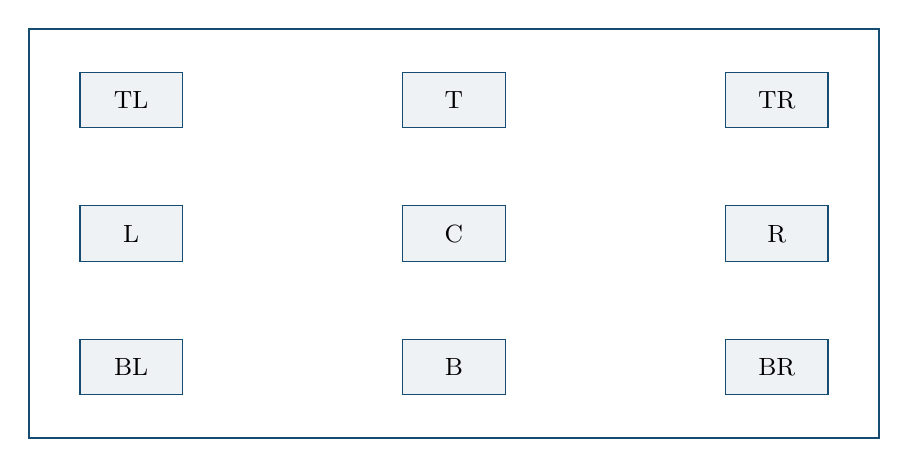
\begin{tikzpicture}[x=1cm,y=1cm,font=\small]
\draw[thick,TemplateBlue] (0,0) rectangle (10.8,5.2);
\foreach \x/\y/\name in {1.3/4.3/TL,5.4/4.3/T,9.5/4.3/TR,
  1.3/2.6/L,5.4/2.6/C,9.5/2.6/R,1.3/0.9/BL,5.4/0.9/B,9.5/0.9/BR} {
  \draw[TemplateBlue,fill=TemplateBlue!7] (\x-0.65,\y-0.35) rectangle (\x+0.65,\y+0.35);
  \node at (\x,\y) {\name};
}
\end{tikzpicture}
\caption{九位置 ROI 布置示意。位置框只表示选点方式，实际 ROI 需落在可测且有效的图卡边缘上。}
\label{fig:quality-roi}
\end{figure}

对于姿态矫正后移出有效视场的位置，记录为“不适用”并说明原因，
不能填为零或在汇总时悄然删除。
黑边和越界填充依据几何有效掩码确定，不能仅按 RGB 为零判定，
因为图卡本身也包含黑色区域。
测试记录以源帧编号关联姿态、有效掩码与 ROI 清单。


\section{基于斜边的 SFR 与 MTF50 清晰度测量}
\subsection{测量方法与计算流程}
SFR 描述图像对不同空间频率的响应。由斜边估计得到的响应包含镜头、传感器、
相机处理、量化与重采样的共同影响，本章将其作为采集至 FPGA 输出链路的清晰度指标。
在未完成线性化和方法核验前，不将其解释为镜头独立的光学 MTF。

对每个 ROI 按以下流程处理，并保存中间数据：
\begin{enumerate}
\item 检查图像无裁剪饱和、明显反光和运动模糊，将像素转为固定定义的亮度或灰度。
若已知相机及输出响应，按实测 OECF 或适当的逆响应完成线性化；
若未知，则记录处理假设，将结果标为当前编码条件下的 SFR，不能直接套用未经核验的 Gamma。
\item 定位斜边并拟合其位置，将 ROI 像素投影到边缘法向，
按亚像素距离分箱形成边缘扩展函数 ESF。记录拟合方式、ROI 大小、倾角和过采样倍数。
\item 对 ESF 求导得到线扩展函数 LSF，按所选算法执行窗函数、
离散微分响应修正和频域归一化，记录所用实现及参数。
\item 计算 SFR 曲线，确定低频归一化响应首次向下穿过 0.5 的频率，
记录 MTF50，并保留边缘过冲、振铃及非单调响应的情况。
\item 对同组重复帧和各个位置重复计算，报告样本数、均值、标准差及最差位置。
剔除异常图像必须使用预先规定的规则，并保留原始帧和剔除原因。
\end{enumerate}

连续形式下的关系可写为
\begin{equation}
\operatorname{LSF}(x)=\frac{\mathrm{d}\operatorname{ESF}(x)}{\mathrm{d}x},\qquad
\operatorname{SFR}(f)=
\frac{\left|\mathcal{F}\{\operatorname{LSF}(x)\}(f)\right|}
{\left|\mathcal{F}\{\operatorname{LSF}(x)\}(0)\right|},
\end{equation}
\begin{equation}
f_{50}=\min\{f>0:\operatorname{SFR}(f)=0.5
\text{，且为首次下降交点}\}.
\label{eq:quality-mtf50}
\end{equation}
实际离散算法还需完成上述窗函数和微分修正，不能只对未经处理的阶跃图像直接做 FFT。
主报告在输出采样的 $0<f\le0.5$ cycles/pixel 范围内给出结果；
若该范围内没有有效 50\% 交点，应记录“范围内未交叉”或“无法可靠估计”，
不能外推填值。ESF 过采样改善估计的相位采样，并不等于输出图像具有更高的独立空间分辨率。

\subsection{频率单位、方向及局部尺度}
主表统一使用 cycles/pixel。若另以图像高度归一化为 LW/PH，须说明线宽口径，
按输出高度 $H$ 使用
\begin{equation}
\operatorname{MTF50}_{\rm LW/PH}=2Hf_{50},\qquad H=1080.
\end{equation}
H 方向的频率响应由近垂直斜边测得，V 方向由近水平斜边测得；
这里 H/V 指频率变化方向，而非边缘延伸方向。

几何矫正会改变局部放大率，直接比较矫正前后的 cycles/pixel 可能把尺度变化
误判为清晰度损失或提升。应记录对应图卡区域在所测方向上的 pixel/mm，
必要时换算为同一物方尺度的 cycles/mm 后比较，或按预先确定的方法统一局部尺度。
用于物方换算的尺度必须对应同一方向及局部区域。
任何额外缩放本身也会引入插值，应另存原生图测量结果并记录缩放方法。
Gamma 开启组单独记录亮度响应和当前曲线，避免与关闭组直接混合平均。

\subsection{清晰度结果记录}
每个姿态、模式和照明条件分别统计表~\ref{tab:quality-mtf} 的指标。
H/V 表示两个测量方向，数值与相应 ROI、曲线和局部尺度关联。
记录项包括测试组、源帧、处理模式、姿态、ROI 尺寸、样本数与线性化方法。

\begin{table}[htbp]
\centering\small
\caption{分区域 MTF50 结果记录（主单位：cycles/pixel）}\label{tab:quality-mtf}
\begin{tabularx}{\textwidth}{>{\raggedright\arraybackslash}p{1.4cm}YYYY}
\toprule
区域 & 原图 H/V & 矫正后 H/V & 局部尺度及比较口径 & ROI/曲线证据 \\
\midrule
中心 C & \qualitypending & \qualitypending & \qualitypending & \qualitypending \\
上 T & \qualitypending & \qualitypending & \qualitypending & \qualitypending \\
下 B & \qualitypending & \qualitypending & \qualitypending & \qualitypending \\
左 L & \qualitypending & \qualitypending & \qualitypending & \qualitypending \\
右 R & \qualitypending & \qualitypending & \qualitypending & \qualitypending \\
左上 TL & \qualitypending & \qualitypending & \qualitypending & \qualitypending \\
右上 TR & \qualitypending & \qualitypending & \qualitypending & \qualitypending \\
左下 BL & \qualitypending & \qualitypending & \qualitypending & \qualitypending \\
右下 BR & \qualitypending & \qualitypending & \qualitypending & \qualitypending \\
\bottomrule
\end{tabularx}
\end{table}

清晰度统计包含逐帧数据、各 ROI 的均值与标准差、外围最差值及测量不确定度。
分析应结合完整 SFR、ESF 和局部边缘图，说明变换尺度、最近邻锯齿及量化的影响，
避免仅用单个 MTF50 数值断言视觉质量全面提高。


\section{网格直线度与残余畸变}
\subsection{直线提取及误差定义}
对网格中的长直线进行亚像素边缘或中心线提取。
宽黑线宜使用两侧边缘确定中心线，并固定算法和阈值，
减少线宽及明暗阈值变化对位置估计的影响。
每条测试线应尽量覆盖较长有效范围，在中心、四边和角部选择横、纵及必要的斜向线。
ROI、端点排除距离、拟合点数、异常点处理和遮挡排除规则应提前确定。

采用正交最小二乘等适合任意方向的拟合方式，得到
\begin{equation}
ax+by+c=0,\qquad a^2+b^2=1.
\end{equation}
对该线上 $n$ 个提取点 $(x_i,y_i)$，定义带符号残差及距离
\begin{equation}
r_i=ax_i+by_i+c,\qquad d_i=|r_i|,
\end{equation}
并计算
\begin{equation}
D_{\rm RMS}=\sqrt{\frac{1}{n}\sum_{i=1}^{n}r_i^2},\qquad
D_{\max}=\max_i d_i,\qquad
D_{95}=\operatorname{percentile}_{95}(d_i).
\end{equation}
若有效测试线段长度为 $L$ 个输出像素，归一化最大直线度误差为
\begin{equation}
\varepsilon_{\rm line}=\frac{D_{\max}}{L}\times100\%.
\label{eq:quality-linearity}
\end{equation}
报告中同时给出像素单位和归一化值，并保留沿线位置对应的带符号残差曲线，
以识别连续弯曲和局部跳变。

透视投影下直线仍为直线，但平行线不一定在图像中保持平行，
线段倾斜也不等于残余畸变。
直线度评价不强行将所有线拟合为水平或垂直；
图卡姿态、校正后视场和投影约定造成的整体倾斜，应与残余弯曲分开说明。
图卡平整度、采集噪声及亚像素提取误差也应计入测量不确定度，
不能仅依据软件输出的小数位数宣称达到对应精度。

\subsection{直线度记录与判定}
每条线均保留原图和矫正后结果，按相同物理线段匹配。
当两者覆盖长度不同或局部尺度变化较大时，应说明像素残差的可比性，
必要时增加同尺度结果；不得通过缩短线段或删除外围采样点来降低残差。

\begin{table}[htbp]
\centering\small
\caption{直线度测量结果（距离单位：pixel）}\label{tab:quality-linearity}
\begin{tabularx}{\textwidth}{>{\raggedright\arraybackslash}p{2cm}YYYYY}
\toprule
线段位置 & 长度/点数 & 原图 RMS & 矫正 RMS & 矫正最大/P95 & 归一化最大误差 \\
\midrule
中央横线 & \qualitypending & \qualitypending & \qualitypending & \qualitypending & \qualitypending \\
中央纵线 & \qualitypending & \qualitypending & \qualitypending & \qualitypending & \qualitypending \\
上/下边缘线 & \qualitypending & \qualitypending & \qualitypending & \qualitypending & \qualitypending \\
左/右边缘线 & \qualitypending & \qualitypending & \qualitypending & \qualitypending & \qualitypending \\
角部代表线 & \qualitypending & \qualitypending & \qualitypending & \qualitypending & \qualitypending \\
\bottomrule
\end{tabularx}
\end{table}

上/下、左/右及四角实测时分别展开记录，不以一个平均值掩盖最差位置。
逐线统计包含 RMS、最大误差、P95、线段长度和最差位置。
直线度结论由测量值、不确定度与预设判据共同决定。


\section{边缘拉伸、断裂与局部完整性}
\subsection{异常拉伸与局部尺度}
使用网格相邻交点间距、方块边长和长宽比检查局部形变，
重点观察四角、姿态边界及有效视场外围。
几何矫正本身会产生预期的尺度变化，所以不能将所有拉伸都认定为缺陷，
也不能要求透视图像中所有网格间距天然相等。
应与相同视场、姿态和采样约定的独立参考，或具有明确成像几何的物方基准比较。

对匹配的局部线段，设输出长度为 $\ell$，参考长度为 $\ell^*$，定义
\begin{equation}
\varepsilon_{\ell}=\frac{|\ell-\ell^*|}{\ell^*}\times100\%.
\end{equation}
横向、纵向分别统计，必要时增加相对于参考长宽比的偏差。
参考线段、交点定位方法、尺度标定和允许误差均应记录。
若未建立独立几何参考，则只保留尺寸分布和观察结论，
不将其填作已经测得的“拉伸误差”。

\subsection{断裂、错位和跨块连续性}
在有效区域内，沿同一条图卡线或方块边缘跟踪连通性，
记录异常缺口数、最大缺口长度和跳变位置。
检测前应确定最小缺口长度、允许的像素连接方式及噪声处理参数，
并对算法检出的异常逐一查看原生像素，避免阈值噪声造成误报。
设计产生的越界黑边、图卡真实间断及被遮挡区域单独标注，不能计作处理断线。

默认输出块大小为 $128\times32$，应重点检查
$x=128k$、$y=32m$ 附近穿过网格线或斜边的位置，
以及图像末行、末列和最后一个不完整块。
对边界两侧比较线条位置、连续性及亮度，检查是否出现整行错位、缓存旧数据或块缝。
最近邻采样可能产生台阶与锯齿，应记录其尺度及可见程度，
并与缺失像素造成的真正断裂区分。

观察统一采用原生 1:1 显示，辅以注明倍率的整数倍最近邻放大，
避免展示软件平滑插值掩盖块缝和缺口。
动态检查则保存连续输出帧或视频，记录姿态、功能切换时刻和异常帧号。

\begin{table}[htbp]
\centering\small
\caption{边缘完整性测量项目}\label{tab:quality-edge}
\begin{tabularx}{\textwidth}{>{\raggedright\arraybackslash}p{3cm}YYY}
\toprule
检查项目 & 区域/条件 & 结果记录 & 局部图/帧号 \\
\midrule
局部横/纵尺度误差 & \qualitypending & \qualitypending & \qualitypending \\
方块长宽比偏差 & \qualitypending & \qualitypending & \qualitypending \\
异常断线数/最大缺口 & \qualitypending & \qualitypending & \qualitypending \\
跨块边界位置跳变 & \qualitypending & \qualitypending & \qualitypending \\
斜边台阶及可见锯齿 & \qualitypending & \qualitypending & \qualitypending \\
末行/末列/不完整块 & \qualitypending & \qualitypending & \qualitypending \\
姿态变化及开关切换 & \qualitypending & \qualitypending & \qualitypending \\
有效覆盖与越界区域 & \qualitypending & \qualitypending & \qualitypending \\
\bottomrule
\end{tabularx}
\end{table}


\section{综合判据与评价结论}
\subsection{门限与验收表}
表~\ref{tab:quality-acceptance} 中的门限应在正式测量前确定。
不同姿态与方向分别判断，主结论使用有效 ROI 中最差位置，
重复测量时同时考虑统计波动及测量不确定度。
若部分位置无法测量，应列出原因及有效视场覆盖，不能默认为通过。

\begin{table}[htbp]
\centering\small
\caption{矫正效果综合评价}\label{tab:quality-acceptance}
\begin{tabularx}{\textwidth}{>{\raggedright\arraybackslash}p{3.2cm}YYY}
\toprule
指标 & 预设判据 & 最差实测结果 & 结论/证据 \\
\midrule
MTF50 与完整 SFR & 未设定 & \qualitypending & \qualitypending \\
直线度 RMS & 未设定 & \qualitypending & \qualitypending \\
最大/归一化直线度 & 未设定 & \qualitypending & \qualitypending \\
局部尺度/长宽比偏差 & 未设定 & \qualitypending & \qualitypending \\
异常断裂与位置跳变 & 未设定 & \qualitypending & \qualitypending \\
原生倍率下边缘观感 & 未设定 & \qualitypending & \qualitypending \\
有效视场覆盖 & 未设定 & \qualitypending & \qualitypending \\
\bottomrule
\end{tabularx}
\end{table}

\subsection{评价结论与数据记录}
本章建立了斜边清晰度、网格直线度和边缘完整性三类评价方法，
分别对应频域响应、几何残差和局部连续性。
中心与外围、水平与垂直、静态与动态条件分组统计，
以有效区域内的最差位置和测量不确定度支撑综合判断。

实物图卡的同源输入输出、逐 ROI 曲线、直线残差及局部放大图尚未形成完整测量记录，
因此表~\ref{tab:quality-mtf}、表~\ref{tab:quality-linearity} 和
表~\ref{tab:quality-edge} 的结果列保留为“未测量”，
表~\ref{tab:quality-acceptance} 不作通过判定。
软件合成图卡与 RTL 功能测试分别验证分析方法和数据通路，
不替代真实相机与 FPGA 输出的定量画质测量。

每组测量采用源帧身份关联输入输出、量化对照、浮点参考、有效掩码和 ROI 坐标，
同时记录曝光、照明、姿态、功能配置、分析方法、原始数据与文件校验值，
保证结果可复核。

\chapter{总结、局限与后续工作}
\section{已完成工作的总结}
本工程已形成面向 1080p 视频的 HDMI 输入、帧自适应 Gamma、RGB565 DDR3 帧缓存、
逐帧姿态快照、定点镜头/姿态逆投影、双槽分块渲染和 HDMI 输出的完整 RTL 通路。
板载 CP2102 支持三个独立功能开关和亮度统计遥测，配置在输入帧边界原子生效。

当前 2026-10-22 基线的完整系统行为模型在给定并发与 DDR 停顿条件下，
达到约 30 个新结果帧/秒；最终 PDS 双角时序及 FIFO Gray 偏斜审计通过。
这些结论支持当前设计在 RTL 与实现工具层面的可行性。
\fillin{补齐实板测量后的最终性能、画质与演示结论}。

\section{赛题完成情况与当前局限}
\begin{table}[htbp]\centering\small
\caption{最终提交前的完成情况核对模板}
\begin{tabularx}{\textwidth}{p{3.1cm}YY}
\toprule
事项 & 当前边界 & 正式提交时补齐 \\
\midrule
视频完整链路 & RTL、实现报告已有；当前候选未板测 & \fillin{板测记录及演示视频} \\
标定参数 & 固定确认的内参与系数 & \fillin{原始标定图集及参数来源说明} \\
切向畸变 & 参数接口保留，当前值为零 & \fillin{非零场景测试或适用范围说明} \\
任意角度能力 & yaw/pitch 每轴约 $\pm15^\circ$，无 roll & \fillin{范围验收、安装标定与扩展状态} \\
重采样与黑边 & 最近邻分块、无效域置黑 & \fillin{双线性需求、画质与黑边验收} \\
实时性与延迟 & 行为模型约 30 fps，实板延迟未测 & \fillin{实板新帧率与端到端数据} \\
图像增强 & 七档帧自适应 Gamma & \fillin{实际光照实验} \\
资源、时序和 CDC & 当前版本有归档结果 & \fillin{最终提交版本与报告对应关系} \\
\bottomrule
\end{tabularx}
\end{table}

运行时串口开关并不是相机内参/畸变参数在线加载接口；当前标定参数由固定配置集成。
如现场要求重新标定相机或修改镜头，应说明参数导出、量化、重新构建及验证过程。

\section{可进一步改进的方向}
后续可围绕分块双线性采样、roll 参与的三轴姿态矩阵、图像/IMU 时间同步、
运行时标定参数加载和更高吞吐开展扩展。稀疏几何网格或倒数 LUT 可作为
精度与资源折中的研究方向，但它们尚不是当前默认路径的已验证功能。

每项改进应分别给出数学误差、边界行为、存储需求和完整系统性能，再重新进行
时序与实板验收。当前最直接的后续工作是完成候选烧录、真实图卡测量和长时稳定性记录。

\guide{正式结论保留已验证且与选题有关的贡献及数值；
删除已完成的待补项，仍未完成的功能如实写入适用范围，不得改写为已达到赛题全部要求。}

\begin{thebibliography}{99}
\addcontentsline{toc}{chapter}{参考资料}
\bibitem{problem} 深圳市紫光同创电子有限公司.
全国大学生嵌入式芯片与系统设计竞赛 2026：FPGA 创新设计赛道选题指南.
选题二：基于紫光同创 FPGA 的任意角度的畸变矫正，正文第 9--12 页.
本地文件：\path{chapter1/reference/problem.pdf}.
\bibitem{project} Pgl50h 工程.
\path{README.md}、\path{EmbFPGA.pds}、\path{src/}，本地查阅日期：2026-10-25.
\bibitem{calibration} 相机标定记录.
\path{calibration/camera_20260930.json}，用户确认的 MATLAB cameraParams，2026-09-30.
\bibitem{current} CP2102 版本位流实现记录.
\path{verification/20261022_pc_control_sbit.md} 及
\path{verification/pds_pc_control_write_ram_20261022/}.
\bibitem{protocol} CP2102 上位机控制与自适应 Gamma 遥测协议.
\path{report/pc_control_protocol.md}，v1，2026-10-21.
\bibitem{history} 1080p30 分块路径历史验证记录.
\path{verification/20261010_pose_tiled_30fps.md}.
\bibitem{board} 深圳市小眼睛科技有限公司.
盘古 50 开发板（MES50HP）硬件使用手册，封面标注 V1.0，2024-07-19.
第 1.1、2.1、2.2.1、2.2.2 节，正文第 2、6--9 页.
本地文件：\path{chapter2/references/} 下的《MES50HP开发板硬件使用手册\_1V1.pdf》.
\bibitem{theory} \fillin{实际查阅的相机模型、标定、图像重采样和 SFR/MTF 测量参考文献，按比赛要求统一格式}.
\end{thebibliography}

\appendix
\chapter{利用 MATLAB 工具箱进行相机标定}
\label{app:camera-calibration}

相机标定为镜头去畸变和姿态逆映射提供焦距、主点及畸变系数。
本附录给出基于 MATLAB Computer Vision Toolbox 的单目标定流程，
说明标定结果如何与第三章算法、FPGA 参数和上位机评估保持一致。
系统采用表~\ref{tab:app-calibration-parameters} 所列标定参数。
原始棋盘格数据集、标定会话与逐图重投影误差记录不完整，
相关采集信息与误差指标据实列为未记录。

\section{标定对象、图卡与采集条件}
\subsection{固定实际成像链路}
标定应使用实际供 FPGA 处理的相机、镜头、分辨率和图像区域。
当前算法与硬件参考尺寸为 $1920\times1080$，像素为方形近似，
采用零 skew 的针孔模型和 Brown 径向/切向畸变。
采集前固定镜头焦距、对焦、曝光、增益及数字变焦，关闭不确定的软件裁切、
自动去畸变和几何缩放；标定与实验使用同一条成像链路。
若相机驱动输出经过裁切或缩放，须把该操作记录为标定条件，
不能仅依据相机型号复用另一尺寸的参数。

标定板使用尺寸准确、表面平整的黑白棋盘格，记录每个方格边长及单位。
MATLAB 中由检测器返回的 \path{boardSize} 是棋盘格方格数，
而上位机评估页面填写的是内角点数：例如 $10\times7$ 个方格对应
$9\times6$ 个内角点。两者必须核对，不能把相同数字直接复制到不同工具。
方格边长决定平移外参的物理单位，焦距和主点仍以像素为单位。

\begin{table}[htbp]\centering\small
\caption{相机标定采集记录}\label{tab:app-calibration-capture}
\begin{tabularx}{\textwidth}{>{\raggedright\arraybackslash}p{3.5cm}Y}
\toprule
项目 & 系统配置与记录状态 \\
\midrule
相机与镜头 & AR0234 相机链路；镜头与设备标识未记录 \\
图像尺寸 & 当前参数用于 $1920\times1080$；未记录 \\
棋盘格 & 未记录 \\
采集环境 & 未记录 \\
数据规模 & 未记录 \\
工具版本 & 未记录 \\
\bottomrule
\end{tabularx}
\end{table}

\subsection{覆盖画面与姿态变化}
标定流程以约 15--25 张清晰图像作为初始采样方案，
实际图像数量由画面覆盖与参数估计稳定性确定。
让棋盘格依次覆盖画面中心、四边与四角，同时改变板到相机的距离和绕两个方向的倾斜。
避免所有图像都正对相机、位于中心或仅绕光轴旋转，因为这些姿态对部分内参约束较弱。

相机与棋盘格在曝光期间保持静止，确保角点无运动模糊、反光、过曝和遮挡。
每次改变位置后保存原始尺寸图像，使用无损格式并保留文件名。
另留若干独立姿态图像作为验证集，不参与参数求解，
用于检查校准后直线是否仍有系统弯曲以及参数能否适用于未见视角。

\section{Camera Calibrator 的操作流程}
在 MATLAB 命令窗口执行 \texttt{cameraCalibrator}，或从 Apps 中打开
Camera Calibrator，按以下顺序操作；菜单名称可能随版本变化\cite{matlab-calibrator}。
\begin{enumerate}
\item 导入同一相机、同一分辨率的棋盘格图像，填写实际方格边长与单位。
核对自动检测出的角点阵列、棋盘方向和图像尺寸，剔除检测错误或模糊图像。
\item 选择与 FPGA 对应的模型：不估计 skew，径向系数数量设为 2，
即 $k_1,k_2$；切向项是否估计需记录。
系统所用切向系数为 $p_1=p_2=0$；求解时是否固定该参数须由标定会话确认。
零系数本身不作为镜头无偏心畸变的物理结论。
\item 执行 Calibrate，查看每张图的重投影误差和相机/标定板外参分布。
检查大误差是否与模糊、反光、板材弯曲或某个画面区域相关，
保留剔除原因，不能只为减小平均误差反复删除边角样本。
\item 查看去畸变预览，检查中心与边缘的网格线。
模型不足时先补充可靠姿态和边缘数据，再比较模型设置；
若必须引入 $k_3$、非零 skew 或其他模型，应同步扩展 FPGA 和软件参考，
不能直接把新参数交给只实现现有模型的链路。
\item 保存标定会话，使用 Export Camera Parameters 将对象导出到工作区，
例如命名为 \texttt{cameraParams}，同时导出参数误差或不确定度信息。
\item 在保留的独立验证图像上检查去畸变结果，归档原图、角点叠加图、
重投影误差图、外参分布和参数文件。
\end{enumerate}

工具箱内部为各张图像同时估计相机内参与标定板外参。
这些外参描述拍摄时标定板相对相机的关系，不是运行时 IMU 输出，
也不等于 IMU 与相机之间的固定安装旋转。

\section{标定模型、误差指标与系统参数}
\subsection{模型与重投影误差}
采用第三章的列向量内参约定，
\begin{equation}
K=\begin{bmatrix}f_x&0&c_x\\0&f_y&c_y\\0&0&1\end{bmatrix},
\qquad L(r)=1+k_1r^2+k_2r^4.
\end{equation}
切向项与式~\eqref{eq:distort-x}、式~\eqref{eq:distort-y} 一致。
对第 $j$ 张图像第 $i$ 个角点，设检测位置为 $\boldsymbol p_{ij}$，
按估计内参、畸变和该图外参投影的位置为 $\hat{\boldsymbol p}_{ij}$，
则本附录定义的重投影 RMS 为
\begin{equation}
e_{\mathrm{RMS}}=
\sqrt{\frac{1}{N_{\mathrm{obs}}}\sum_{j,i}
\|\boldsymbol p_{ij}-\hat{\boldsymbol p}_{ij}\|_2^2}.
\label{eq:app-calibration-rms}
\end{equation}
单位为 px，$N_{\mathrm{obs}}$ 为有效角点观测总数。
工具箱的 \path{MeanReprojectionError} 是平均重投影误差统计，
不能不加区分地标作式~\eqref{eq:app-calibration-rms} 的 RMS\cite{matlab-camera-parameters}。
本附录导出程序分别保存这两个量，并使用不同字段名。

误差应同时按图像、画面位置和方向分析。
总体均值较小但边角残差明显偏向同一方向，可能说明覆盖不足或模型不匹配。
同一组角点上的拟合残差只说明模型拟合程度，
还应检查独立验证图像、参数稳定性及实际直线度；
标定重投影误差也不能替代第~\ref{chap:performance}~章的 MTF50/SFR 测量。

\subsection{系统采用的标定参数}
\begin{table}[htbp]\centering\small
\caption{相机标定参数及坐标约定}\label{tab:app-calibration-parameters}
\begin{tabularx}{\textwidth}{>{\raggedright\arraybackslash}p{3.4cm}YY}
\toprule
参数 & 数值 & 含义 \\
\midrule
图像尺寸 & $1080\times1920$（高$\times$宽） & 与工程全幅输入一致 \\
$f_x,f_y$ & $748.4469,\ 748.0773$ & 像素焦距 \\
$c_x,c_y$ & $944.9033,\ 522.3963$ & MATLAB 一起点主点坐标 \\
$k_1,k_2$ & $0.0099,\ -0.0434$ & 径向系数，无量纲 \\
$p_1,p_2$ & $0,\ 0$ & 切向系数；原始求解设置未记录 \\
输出内参 & 与输入相同 & 当前不另做裁切或焦距调整 \\
标定误差与样本数 & 未记录 & 参数文件不含该统计 \\
\bottomrule
\end{tabularx}
\end{table}

表~\ref{tab:app-calibration-parameters} 的 MATLAB 参数文本与 FPGA 标定 JSON 一致，
适用于 $1920\times1080$ 输入及对应像素坐标约定。
\sourcefile{\path{chapter3/reference/undistort/para.txt}；
\path{../Pgl50h/calibration/camera_20260930.json}}

\section{参数导出与坐标转换}
\subsection{保存 MATLAB 对象与上位机可读文件}
本附录提供 \path{export_camera_calibration.m}，在完成工具箱标定并导出对象后执行：
\begin{quote}\small\ttfamily
addpath('appendix/appendixA');\\
export\_camera\_calibration(cameraParams, 'calibration\_export');
\end{quote}
程序保存 \path{cameraParams.mat} 和 \path{camera_calibration.json}。
MAT 文件保留工具箱对象；JSON 保存 MATLAB 形式的内参、两项径向系数、
两项切向系数、图像高宽和像素起点声明，可由附录~\ref{app:pc-host}~的上位机读取。
该导出配置要求零 skew、两个径向系数，避免默默丢弃第三个径向项。
导出程序用于统一数据格式，未列入已执行的 MATLAB 验证项目。
系统采用的标定数值来自表~\ref{tab:app-calibration-parameters} 的参数文件。

JSON 的关键字段与现有工程一致：
\begin{table}[htbp]\centering\small
\caption{标定 JSON 与不同程序间的数据约定}\label{tab:app-calibration-json}
\begin{tabularx}{\textwidth}{>{\raggedright\arraybackslash}p{5.4cm}Y}
\toprule
字段 & 约定 \\
\midrule
\path{image_size_hw} & MATLAB 图像尺寸 $[H,W]$，不是 OpenCV 的 $[W,H]$ \\
\path{intrinsic_matrix_matlab} & 传统 \path{cameraParameters.IntrinsicMatrix}，为本报告 $K$ 的转置 \\
\path{radial_distortion} & $[k_1,k_2]$ \\
\path{tangential_distortion} & $[p_1,p_2]$ \\
\path{pixel_coordinate_origin} & 明确写入 1，表示 MATLAB 像素中心从 1 开始 \\
\path{mean_reprojection_error_px} & 工具箱平均重投影误差 \\
\path{reprojection_rms_px} & 若有逐点残差，则按式~\eqref{eq:app-calibration-rms} 计算 \\
\bottomrule
\end{tabularx}
\end{table}

\subsection{MATLAB、OpenCV 与 FPGA 对齐}
旧式 MATLAB \path{IntrinsicMatrix} 需要转置后才能用于本报告的列向量公式。
R2022b 起提供的 \path{K} 已采用列向量约定，不应再次转置；
导出程序按对象属性选择相应分支\cite{matlab-camera-parameters}。
将 MATLAB 像素中心 $(u_M,v_M)$ 转为从零开始的坐标时，
\begin{equation}
u_0=u_M-1,\quad v_0=v_M-1,\qquad
K_0=\begin{bmatrix}
f_x&0&c_x-1\\0&f_y&c_y-1\\0&0&1
\end{bmatrix}.
\end{equation}
因此，上位机转换后的零起点主点为 $(943.9033,521.3963)$，
焦距和畸变系数不变。
OpenCV 的常用五项系数顺序为 $[k_1,k_2,p_1,p_2,k_3]$，
当前 $k_3=0$；它与“径向数组后接切向数组”的顺序不同。

FPGA 可以在建立视线时将零起点像素加 1，或使用主点减 1 后的 $K_0$，
两种做法应选择一种并贯穿映射与采样，避免重复补偿。
若零起点图像裁去左侧 $x_0$ 列、上侧 $y_0$ 行，主点应相应减去 $(x_0,y_0)$。
若还发生缩放或平移，使用与实际像素中心规则对应的变换矩阵 $A$ 更新 $K'=AK_0$，
不能仅修改分辨率字段。工具箱去畸变输出采用不同视场时，也应记录新的内参与输出原点。

\section{参数进入 FPGA 与实验归档}
上位机导入 JSON 只更新 PC 侧参考，不会向 FPGA 下载标定参数。
更换标定后，应同时核对软件参考、RTL 中的定点常量、有效视场和分块缓存窗口，
运行相应功能回归与完整链路测试，再生成新的实现报告和位流。
参数集成对象为默认联合逆投影器及其调用参数，确保软件参考与硬件常量一致。

标定数据记录包括原始图像、文件清单、图卡尺寸、采集条件、工具箱会话、
MAT 对象、JSON、残差图及独立验证结果，并保存参数文件 SHA256。
测量结果与 FPGA 源码、约束和配置位流关联。
原始角点检测、重投影残差、外参分布及独立验证图未纳入现有记录，
因此本附录不报告标定 RMS 或样本数的数值结论。
\sourcefile{\path{appendix/appendixA/export_camera_calibration.m}；
\path{../PC/fpga_host/evaluation/calibration.py}；
\path{chapter3/reference/common/simulation_config.m}}

\chapter{利用 IMU 获取摄像头姿态}
\label{app:attitude-estimation}

摄像头姿态由与其刚性连接的 BMI088 测量，经 STM32F4 解算后分别发送给 FPGA 和 PC。
本附录依据 \path{../Stm32f4/} 中的采集、Mahony 解算和通信源码，
说明从惯性数据到摄像头矫正参数的处理过程。
当前工程提供 yaw、pitch、roll 三个姿态角，没有估计摄像头平移位置，
因此本附录中的“位姿获取”具体实现为旋转姿态获取。
默认 FPGA 使用 yaw/pitch，roll 仅保留接收与显示。

\section{硬件接口与任务组织}
\subsection{传感器采集链路}
STM32 工程使用 STM32F407 系列，配置系统时钟为 168 MHz，
基于 HAL、FreeRTOS 与 CMSIS-RTOS2 组织任务。
BMI088 的加速度计与陀螺仪共享 SPI1，使用独立片选；
数据就绪中断启动 SPI DMA，发送/接收完成回调释放总线及数据缓冲。
温度由定时器触发读取，TIM10 PWM 驱动加热控制，代码目标温度为 $36\,^{\circ}\mathrm C$。
该温度是控制设定值，不能代替实测的温度稳定度或零偏稳定度。

\begin{table}[htbp]\centering\small
\caption{STM32 IMU 接口与解算配置}\label{tab:app-imu-config}
\begin{tabularx}{\textwidth}{>{\raggedright\arraybackslash}p{3.5cm}YY}
\toprule
项目 & 当前代码配置 & 说明 \\
\midrule
传感器总线 & SPI1，DMA 读写 & 两个传感器独立片选，以信号量协调共享总线 \\
加速度计 & $\pm3g$，800 Hz ODR & 数据转换系数为 $0.00089685$，用于换算为 $\mathrm{m/s^2}$ \\
陀螺仪 & $\pm1000\,^{\circ}/\mathrm s$，1000 Hz ODR & 寄存器宏为 \path{GYRO_RANGE_1000_DEG_S}；灵敏度 32.768 LSB/(${}^{\circ}/\mathrm s$) \\
解算周期 & 1 tick，tick 频率 1000 Hz & Mahony 源码固定使用 $\Delta t=0.001$ s \\
温度控制 & 目标 $36\,^{\circ}\mathrm C$，PWM 加热 & 需上板记录升温时间和稳态波动 \\
FPGA 姿态链路 & USART6，PG14 TX，921600 baud & 8-N-1，10 字节姿态帧，目标 50 Hz \\
PC 姿态链路 & USB FS CDC，目标 50 Hz & 上位机使用 115200/8-N-1 线路设置；不代表 USB 物理比特率 \\
\bottomrule
\end{tabularx}
\end{table}

量程以实际写入宏和换算系数为准：源码有一处陀螺仪量程注释写为
$\pm500\,^{\circ}/\mathrm s$，但实际配置为
\path{GYRO_RANGE_1000_DEG_S}，转换也采用 32.768。
记录实验时应按后者核对，避免用错误灵敏度将角速度缩放一倍。

\subsection{解算与双通道分发}
\path{AppBmi088Task} 完成初始化和上电等待后，每 1 ms 目标周期调用
\path{control()}、\path{temp_control()} 和 \path{callback()}，
分别解析数据、更新温控和进行姿态解算。
随后把 roll、pitch、yaw 三个浮点数复制到两条独立状态队列，
供 \path{AppJetsonTask} 与 \path{AppJetsonUsbTask} 读取。
代码中的 Jetson 命名沿用早期模块名，当前分别承担 USART 与 USB CDC 姿态发送。

\begin{figure}[htbp]\centering
\begin{tikzpicture}[font=\small,
  box/.style={draw=TemplateBlue,rounded corners,align=center,minimum height=1.05cm},
  flow/.style={-{Stealth[length=2mm]},thick}]
\node[box,text width=1.8cm] (imu) {BMI088\\加速度/角速度};
\node[box,text width=3.0cm,right=0.45cm of imu] (solve) {SPI DMA / STM32\\零偏扣除与 Mahony};
\node[box,text width=1.8cm,right=0.45cm of solve] (queue) {姿态快照\\双队列};
\node[box,text width=3.0cm,right=0.65cm of queue,yshift=0.75cm] (uart) {USART6，50 Hz\\FPGA 帧级锁存};
\node[box,text width=3.0cm,below=0.45cm of uart] (usb) {USB CDC，50 Hz\\PC 解码与模型显示};
\draw[flow] (imu) -- (solve);
\draw[flow] (solve) -- (queue);
\draw[flow] (queue.east) -- ++(0.22,0) |- (uart.west);
\draw[flow] (queue.east) -- ++(0.22,0) |- (usb.west);
\end{tikzpicture}
\caption{现有固件的姿态采集、解算与双通道分发}
\label{fig:app-imu-pipeline}
\end{figure}

两条队列深度均为 2，生产者非阻塞投递，消费者每 20 ms 取一次 FIFO 数据，
不是每次循环都清空队列并选取最新值。
因此，50 Hz 是通信任务的目标频率，不能认为每个发送值都来自该时刻最新的惯性采样。
800 Hz 加速度、1000 Hz 陀螺仪与 1000 Hz 解算循环也不是同一事件，
当前代码可能在某次循环中重用上一组已读数据。
初始化前就已取得调度基准，而初始化包含较长等待，且任务未检查 \path{setup()} 返回状态，
因此代码中的目标周期不构成启动后稳定 1 kHz 或传感器就绪的保证；
后续固件应在初始化成功后重新设定调度基准，并记录采样有效性。
正式动态测试应测量采集新鲜度和任务抖动，而非仅用任务周期推算角度延迟。
\sourcefile{\path{../Stm32f4/Core/Hardware/bmi088/bmi088_task.cpp}；
\path{../Stm32f4/Core/Src/freertos.c}；
\path{../Stm32f4/Core/Hardware/jetson/jetson_task.cpp}；
\path{../Stm32f4/Core/Hardware/jetson_usb/jetson_usb_task.cpp}}

\section{惯性数据处理与 Mahony 姿态解算}
\subsection{单位转换、零偏与温度}
陀螺仪三轴按 x/roll、y/pitch、z/yaw 排列。
设原始有符号输出为 $g_{\mathrm{raw},i}$，灵敏度为 $s_g=32.768$，
固件转换为弧度每秒并扣除偏置：
\begin{equation}
\omega_i=\frac{g_{\mathrm{raw},i}}{s_g}\frac{\pi}{180}-b_i.
\end{equation}
当前构造函数中的固定偏置为
\begin{equation}
\boldsymbol b=
[0.00155281043,\ 0.00148057903,\ 0.00126652408]^{\mathsf T}
\ \mathrm{rad/s}.
\end{equation}
这些数值是已有代码常量，没有随附本次器件、温度和采样时长的原始校准记录，
更换传感器后应重新测量，不能当作所有 BMI088 的通用校准值。
建议在安装固定、温度稳定后采集静态角速度，以均值估计偏置，
另用独立时段记录扣偏后的均值和标准差。

加速度计输出按量程系数转换后用于估计重力方向。
可通过多面静置检查轴向、符号、零偏与尺度，
在运动中则应注意非重力加速度会影响姿态反馈。
现有实现没有完整的六面加速度校准流程，也没有根据动态加速度自适应调整反馈权重；
大幅平移、振动或急停下的误差需另行验证。

\subsection{四元数更新与角度输出}
Mahony 算法用陀螺仪积分提供短时姿态变化，
以归一化加速度与估计重力方向之间的叉乘误差修正漂移。
其处理可概括为
\begin{align}
\boldsymbol e&=\hat{\boldsymbol a}\times\hat{\boldsymbol g}(q),\\
\boldsymbol\omega_c&=\boldsymbol\omega+
K_P\boldsymbol e+K_I\int\boldsymbol e\,dt,\\
\dot q&=\tfrac12q\otimes[0,\boldsymbol\omega_c],\qquad
q_{n+1}=\operatorname{normalize}(q_n+\dot q\,\Delta t).
\end{align}
这里以单位重力向量写出原理；源码使用 half-vector 和 \path{twoKp/twoKi} 的等价写法，
默认 \texttt{twoKp=1.0}、\texttt{twoKi=0}，固定采样频率为 1000 Hz。
初始四元数为 $[1,0,0,0]$，每次更新后归一化，再按源码的欧拉角公式输出弧度。

当前调用向磁力计通道传入三个零值，实际进入六轴 IMU 分支，
重力可约束俯仰与横滚，但无法提供绕重力方向的绝对航向参考。
因此，yaw 只适合作为相对旋转观测，长期漂移应测量并记录。
默认积分反馈关闭，不能把 Mahony 结构本身描述为已经完成在线陀螺仪零偏估计。
固定 $\Delta t$ 也要求实际任务周期与 1 ms 一致，
调度阻塞和丢采样会引入额外误差。
\sourcefile{\path{../Stm32f4/Core/Hardware/bmi088/bmi088.cpp}；
\path{../Stm32f4/Core/Hardware/bmi088/MahonyAHRS.c}；
\path{../Stm32f4/Core/Hardware/bmi088/bmi088_temperature.cpp}}

\section{IMU 安装坐标与摄像头姿态}
\subsection{刚性安装与参考零位}
IMU 应与摄像头刚性连接，标明传感器三轴、相机光轴、图像向右和向下的方向，
避免安装支架松动或线缆牵拉改变两者关系。
通过绕机械轴的单轴正负转动，确认输出角度及矫正图像的方向。
STM32 的 yaw 绕传感器 z 轴，不能仅因字段名相同就等同于图像算法的水平偏转角；
安装后可能需要轴置换、符号转换和固定旋转补偿。

设 $R_{AB}$ 将 B 坐标表达转换到 A 坐标表达，S 为 IMU、C 为相机，W 为参考坐标系。
若已确认解算四元数对应的 $R_{WS}(t)$ 方向，且已标定固定安装旋转 $R_{SC}$，则
\begin{equation}
R_{WC}(t)=R_{WS}(t)R_{SC}.
\end{equation}
以零位相机 $C_0$ 作为理想输出视角，输出视线到当前源相机 $C_t$ 的旋转应为
\begin{equation}
R_{C_tC_0}=R_{WC}(t)^{\mathsf T}R_{WC}(0)
=R_{SC}^{\mathsf T}R_{WS}(t)^{\mathsf T}R_{WS}(0)R_{SC}.
\label{eq:app-imu-camera-rotation}
\end{equation}
该式说明安装旋转、参考零位及映射方向的关系。
当前固件仅发送三个欧拉角，没有显式应用这条完整的相机外参链，
因此式~\eqref{eq:app-imu-camera-rotation} 是联调与后续完善的坐标依据，
不能描述为当前已完成的外参标定功能。

\subsection{与默认 FPGA 路径对接}
当前 FPGA 默认按 yaw/pitch 每轴约 $\pm15^\circ$ 工作，roll 不参与逆映射。
联调应使用该范围内的单轴与组合角度，逐项记录
“机械转动方向、STM32 读数、发送字段、FPGA 矫正方向”，
并核对第三章的旋转顺序。
超过范围时应检查限幅和无效视场处理，不能用通信协议可编码约 $\pm\pi$ 的能力
推断系统支持同样大的有效矫正视场。

上位机“当前姿态设为模型零点”只改变 PC 模型显示，
不会修改 STM32 偏置、FPGA 参考姿态或发送数据。
更严格的姿态零位应通过旋转矩阵或四元数建立相对关系；
简单逐项减欧拉角只在受限小角度、已统一顺序的条件下近似适用。
\fillin{补充 IMU 与相机安装照片、三轴示意、安装旋转或轴映射表及参考零位定义。}

\section{姿态帧、传输通道与异常处理}
\subsection{十字节二进制帧}
USART6 与 USB CDC 使用相同的载荷格式：
\begin{center}\small
\texttt{55 AA | Yaw\_L Yaw\_H | Pit\_L Pit\_H | Rol\_L Rol\_H | SUM | 0D}
\end{center}
每个角度先归一化到 $[-\pi,\pi)$，乘以 2048 后按最接近整数取整，
半整数向远离零的方向处理，编码为小端有符号 16 bit 补码。
接收端换算为
\begin{equation}
\theta_{\mathrm{rad}}=\frac{\operatorname{int16}(\mathrm{raw})}{2048},
\qquad
\theta_{\mathrm{deg}}=\theta_{\mathrm{rad}}\frac{180}{\pi}.
\end{equation}
量化步长为 $1/2048$ rad，约 $0.027976^\circ$，
这只是通信分辨率，不是传感器测量精度。
SUM 为偏移 2--7 六个无符号字节的累加和低 8 位，
不包含帧头与帧尾；它不是 XOR 或 CRC。

例如 yaw=$90^\circ$、pitch=$-30^\circ$、roll=$15^\circ$ 的编解码样例为
\begin{center}\small\texttt{55 AA 91 0C D0 FB 18 02 82 0D}。
\end{center}
此例用于核对字节序、符号与校验，不代表默认 FPGA 的有效矫正范围。
三个解码值受量化影响，约为 $90.0003^\circ$、$-29.9908^\circ$、$14.9954^\circ$。

\subsection{两条发送链路的区别}
USART6 的 921600 baud 是真实异步串口速率，10 字节、8-N-1 的一帧在线路上约需
$100/921600=108.5\ \mu\mathrm s$，远小于 20 ms 目标发送周期。
USB CDC 的 115200 是主机线路编码设置，不能据此计算 USB 的实际传输时间。
USB 路径检查设备已配置且上一笔发送完成后才重用发送缓冲，忙时跳过本次机会；
两条链路均未提供应用层逐帧确认与补发。

接收端必须按连续字节流处理半包、粘包和噪声。
找到 \texttt{55 AA} 后等满 10 字节再检查帧尾与校验，
错误时仅向前移动一个字节重新搜索，不能用文本行或 USB 包边界分帧。
角度跨越 $\pm\pi$ 时会出现数值回绕，计算连续轨迹和角速度前需展开角度。

当前帧不含采样时间戳、序号、传感器就绪位或安装标识。
首次姿态数据到达前可能发送零值，队列无更新时可能继续发送旧姿态；
所以“收到合法帧”不等于“传感器已就绪且数据新鲜”。
PC 连续 0.5 s 无合法帧时提示超时，但这仍是通信层检查。
后续若需要严格动态对齐，应扩展采样序号、硬件时间戳和有效状态，并同步升级 FPGA 与 PC 解码。
\sourcefile{\path{../Stm32f4/Core/Hardware/jetson/jetson.cpp}；
\path{../Stm32f4/Core/Hardware/jetson_usb/jetson_usb.cpp}；
\path{../Stm32f4/Core/Hardware/jetson_usb/usb_receive_manual.md}；
\path{../PC/fpga_host/core/protocols.py}}

\section{联调步骤与测量记录}
先固定相机与 IMU，等待温度和姿态趋于稳定，检查静置时三轴数据，
再分别执行正负 yaw/pitch 及组合转动。
用机械角度参考或独立姿态参考比较读数，
并同时抓取 USART 与 USB 帧，核对两条链路的编码一致性及数据更新时间。
开启 FPGA 姿态矫正后检查图卡方向、帧内稳定性和失联行为，
不将 PC 模型运动正确作为相机矫正方向正确的唯一依据。

\begin{table}[htbp]\centering\small
\caption{IMU 到摄像头姿态的实测记录模板}\label{tab:app-imu-measurements}
\begin{tabularx}{\textwidth}{>{\raggedright\arraybackslash}p{3.1cm}YY}
\toprule
项目 & 测量方法与记录内容 & 当前记录 \\
\midrule
静态零偏与噪声 & 温度稳定后记录三轴均值、标准差和采样时长 & \fillin{待测} \\
角度准确度 & 已知正负单轴角度与组合姿态；报告偏差及重复性 & \fillin{待测} \\
航向漂移 & 静置连续记录，展开 yaw 后统计指定时长内漂移 & \fillin{待测} \\
温控效果 & 目标温度、升温时间、稳态波动与环境温度 & \fillin{待测} \\
采样与通信节拍 & 实际有效帧率、接收间隔分布、丢包与重复值 & \fillin{待测} \\
姿态到画面响应 & 阶跃转动、串口到达、FPGA 帧锁存及显示事件 & \fillin{待测} \\
异常恢复 & 断开、重连、错误校验、启动全零及长期无更新 & \fillin{待测} \\
\bottomrule
\end{tabularx}
\end{table}

第五章已验证 FPGA 姿态 UART 的符号、小端、校验拒收及跨域快照，
附录~\ref{app:pc-host}~给出上位机姿态解析与软件检查。
这些测试覆盖协议与软件行为，表~\ref{tab:app-imu-measurements} 的实物精度和动态响应
仍须按同一固件、安装和温度条件实际填写。

\chapter{上位机软件研发与使用}
\label{app:pc-host}

上位机为 FPGA 图像矫正系统提供视频对照、运行时控制、Gamma 遥测、
IMU 姿态显示和图卡评估入口。本附录依据 \path{../PC/} 中的 Python 工程，
介绍软件结构、关键实现与联调方法。
软件以 Python 3.10 及以上版本、PySide6/Qt 为界面基础，
通过 OpenCV、NumPy 和 pyserial 完成图像分析、模型变换及串口通信。
现有版本为 0.1.0，使用的模型、协议和参考资料保存在 \path{Device/} 中。

\section{功能范围与设备连接}
\subsection{两路视频与两条串口}
系统由原始相机、PC 副屏、FPGA、HDMI 采集卡及 STM32 组成。
原始相机通过 USB 接入 PC，其实时图像可经副屏 HDMI 送入 FPGA；
FPGA HDMI 输出通过独立 USB 采集卡回到 PC，与原始预览并排显示。
PC 与 FPGA 的 CP210x 串口用于控制和统计，
PC 与 STM32 的 USB CDC 用于接收姿态；图像不经过这两条串口传输。

\begin{table}[htbp]\centering\small
\caption{上位机设备接口与数据用途}\label{tab:app-host-devices}
\begin{tabularx}{\textwidth}{>{\raggedright\arraybackslash}p{3.0cm}>{\raggedright\arraybackslash}p{3.0cm}Y}
\toprule
设备 & 识别参考 & 数据与连接要求 \\
\midrule
AR0234 USB 相机 & VID:PID \texttt{1bcf:2cd1} & 原始视频，目标采集请求 $1920\times1080$、60 fps \\
UGREEN 25854 & \texttt{2b89:5854} & 采集 FPGA HDMI 输出，独立于原相机视频节点 \\
FPGA CP210x & \texttt{10c4:ea60} & 115200/8-N-1，无流控；功能掩码、状态和 Gamma 统计 \\
STM32 Virtual COM & \texttt{0483:5740} & 115200/8-N-1 线路设置；十字节姿态协议 \\
PC 独立副屏 & 显示器名称与实际信号模式 & 扩展桌面，$1920\times1080$、约 60 Hz，连接 FPGA 输入 \\
\bottomrule
\end{tabularx}
\end{table}

设备 VID/PID 用于首次发现和建议，不能替代唯一身份识别。
多个同型号串口、同一相机的多个视频节点都需人工核对。
Linux 通常使用 \path{/dev/videoN}、\path{/dev/ttyUSB0} 或 \path{/dev/ttyACM0}，
Windows 使用相机索引和 \texttt{COM} 端口。
FPGA 位流必须支持当前协议；STM32 的 USART6 到 FPGA 链路为 921600 baud，
与表~\ref{tab:app-host-devices} 中 PC 打开的两个串口设置不同。

\subsection{界面组织}
主页仅放置原始图像、处理图像与状态，
设备/对照、FPGA/Gamma、云台姿态、日志分别通过顶部按钮打开独立非模态窗口。
这种布局使双图保持较大显示面积，同时保留控制和故障信息。
“标定评估”使用独立页签，切换时先停止并清理当前设备任务，
避免两套流程同时占用视频设备或重复运行评估线程。

\begin{figure}[htbp]\centering
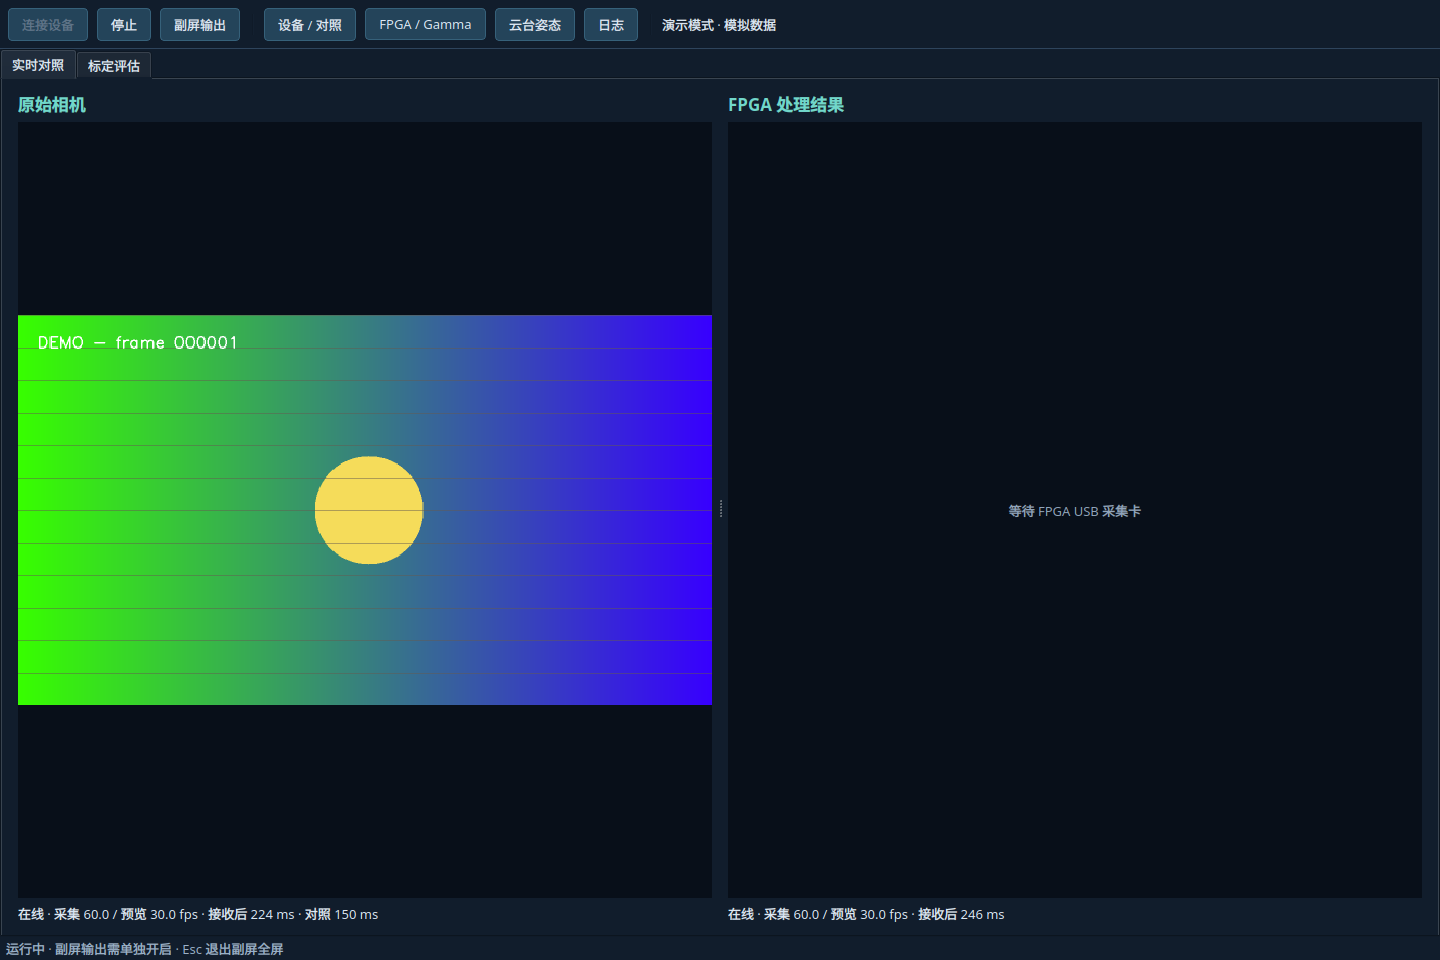
\includegraphics[width=\textwidth]{appendix/appendixC/figures/host_demo.png}
\caption{上位机主页布局（引用工程演示模式截图，画面和状态均不作为硬件测量数据）}
\label{fig:app-host-demo}
\end{figure}

\section{软件分层与并发设计}
\subsection{模块划分}
\begin{table}[htbp]\centering\small
\caption{上位机代码结构与职责}\label{tab:app-host-architecture}
\begin{tabularx}{\textwidth}{>{\raggedright\arraybackslash}p{3.0cm}Y}
\toprule
目录或模块 & 实现职责 \\
\midrule
\path{app.py}、\path{config.py} & 启动参数、设备发现、配置校验及 JSON 原子保存 \\
\path{core/protocols.py} & FPGA 包与 IMU 字节流的编解码、状态和统计数据类型 \\
\path{core/requests.py} & 单个未完成请求门控、序号匹配与超时 \\
\path{core/buffering.py}、\path{jpeg.py} & 带本地时间的有界历史、JPEG 增量分帧 \\
\path{core/model.py} & URDF/STL 资源解析、关节变换和显示网格简化 \\
\path{devices/} & 视频/串口后台 I/O、设备生命周期、演示数据及评估调度 \\
\path{evaluation/} & 标定文件转换、棋盘格检测、几何误差与相对 SFR；不依赖 Qt \\
\path{ui/} & 双图显示、独立工具窗口、评估结果和用户操作 \\
\bottomrule
\end{tabularx}
\end{table}

协议层与 I/O、界面分离，便于在没有 FPGA 或相机时测试解析器。
工作线程通过带锁快照发布状态，Qt 对象只在主线程更新。
视频采用最新帧邮箱和有界历史，界面定时拉取，
不为每个采集帧排队发送大量绘制事件，以防界面阻塞后积累过期图像。

\subsection{采集、预览和副屏分别调度}
每个视频源将连续读取、预览解码和全尺寸输出解码分开。
Linux 自动后端优先使用 FFmpeg/V4L2；MJPG 模式直接保留设备输出的 JPEG，
读取线程不做全尺寸解码或重新编码。
JPEG 分帧器支持分块输入、转义、重启标记和渐进多扫描，限制单帧大小，
不能简单搜索所有字节中的 \texttt{FFD8/FFD9} 代替完整分帧。
其他支持格式包括 YUYV、NV12，并提供 OpenCV 后端。

主页预览后台最多约 30 Hz，MJPG 先半尺寸解码再缩至 $640\times360$；
处理跟不上时跳过旧帧，保持最新画面。
副屏可见时独立解码最新全尺寸原始帧，使用 16 ms 定时器请求绘制，
不读取主页的对照延时。
采集卡只用于处理结果预览，不反向成为 FPGA 输入源。

原始相机历史最多保留 2.5 s 且不超过 128 MiB，
采集卡历史最多 0.25 s 且不超过 128 MiB；实际时间范围可能因码率提前缩短。
MJPG 历史保存压缩帧，其他格式保留缩小预览历史。
断连增加会话标识，后台结果只有在会话和设置仍匹配时才发布，
防止旧解码任务在清空后重新填入过期帧。

\subsection{延时对照与性能数据含义}
对照延时范围为 0--2000 ms，默认 150 ms，
只延迟原图预览，以便人工对齐 FPGA/采集卡链路的较晚画面。
选帧依据 PC 本地单调时钟，不具备硬件帧配对能力。
实时性检查时应将该值设为 0 ms，并分别观察实际采集率、预览发布率和帧龄。

界面的“接收后”时间从 PC 收到输入帧开始计，
包含配置延时、解码和界面调度，不包含设备内部或 USB 上游时间，
不能作为 FPGA 端到端延迟。
同样，请求 1080p60、每 16 ms 请求绘制和实际 HDMI 输出频率是不同事件；
副屏物理时序应在操作系统显示设置中确认，应用不会自动修改显示模式。
\sourcefile{\path{../PC/fpga_host/devices/video.py}；
\path{../PC/fpga_host/devices/video_sources.py}；
\path{../PC/fpga_host/core/buffering.py}；
\path{../PC/docs/development.md}}

\section{FPGA 控制与 Gamma 遥测}
\subsection{协议与帧边界生效}
FPGA 控制包使用二进制格式
\begin{center}\small
\texttt{A5 5A | VERSION | TYPE | SEQ | LEN | PAYLOAD | XOR}。
\end{center}
VERSION 为 \texttt{01}，XOR 从 VERSION 到载荷末尾逐字节异或，
多字节统计字段为小端。
\texttt{SET\_FEATURES/GET\_STATUS/SET\_STREAM/GET\_SNAPSHOT}
分别为 \texttt{10/11/12/13}，返回
\texttt{STATUS/GAMMA\_STATS} 为 \texttt{80/81}，以上编号均为十六进制。
STATUS 负载为 8 字节，Gamma 统计负载为 28 字节。

功能掩码 bit0、bit1、bit2 分别控制去畸变、姿态矫正和自动 Gamma，
上位机一次提交完整三位掩码，禁用设备 \path{available_mask} 不支持的位。
界面同时显示 requested、applied 和 pending：请求已接收后，
还要等输入 SOF 才应用于后续完整输入帧。
applied 变化也不意味着该帧的矫正结果已经出现在 HDMI 上。

\path{RequestGate} 只允许一个未完成请求，
只有序号匹配且负载合法的 STATUS 才释放门控；
异步 Gamma 统计或旧序号响应不能冒充 ACK。
连接后及每 250 ms 查询状态，用户命令优先于下一次轮询，
pending 期间禁止重复提交 SET，仍允许查询和遥测操作。
1 s 内未收到匹配响应时断开，约 2 s 后重连并查询实际状态，
不自动重放 SET，以应对命令已执行但 ACK 丢失的情况。

\subsection{亮度统计与新鲜度}
遥测包括输入帧编号、有效像素数、增强前后亮度和、
增强前暗部/高光计数、实际/目标曲线与该帧功能掩码。
平均亮度与比例分别由亮度和、计数除以有效像素数得到，
分母为零时显示无效，不能显示为零亮度。
暗部和高光比例都来自增强前图像，不能直接解释为增强后比例改善。

Gamma 曲线视图按协议公式绘制示意，
不是从 FPGA LUT 逐项读取的结果；关闭增强时显示恒等映射。
软件分别记录最近合法统计包接收时间和最近帧编号变化时间，
避免重复发送旧统计时误报“图像持续更新”。
这些统计属于输入 Gamma 阶段，不能与最终 HDMI 显示帧默认建立一一对应。
\sourcefile{\path{../PC/fpga_host/core/protocols.py}；
\path{../PC/fpga_host/core/requests.py}；
\path{../PC/fpga_host/devices/serial_link.py}；
\path{../PC/Device/fpga_uart/reference/pc_control_protocol.md}}

\section{姿态解码与三维模型显示}
STM32 接收端按附录~\ref{app:attitude-estimation}~的十字节协议增量解码，
支持半帧、多帧、噪声与错误校验后的重新同步。
三轴补码除以 2048 得到弧度，再转换成界面角度；
连续 0.5 s 无合法帧时标记超时，数值置为无效，模型保留最后姿态。
由于协议没有采样时间戳和就绪位，即使通信持续，也不能确认传感器数据持续更新。

模型视图读取已有 URDF 与 STL，按 joint origin、axis 和关节层级组合刚体变换，
支持资源中的 \texttt{package://} 路径，不依赖 ROS 或 OpenGL。
当前 yaw/pitch 关节随姿态运动，原模型无 roll 关节，roll 仅以读数显示。
视图采用 CPU QPainter 正交投影、深度排序和简化网格，用于观察方向和零位。

用户可设置 yaw/pitch 显示方向，并将当前姿态设为模型零点。
该操作只影响本次连接中的 PC 显示，不会改变原始读数、固件校准或 FPGA 矫正参数，
断开后零点清除。
模型显示也不包含已标定的相机--IMU 外参，
必须按实际安装完成轴向检查后，才可辅助判断相机姿态。
\sourcefile{\path{../PC/fpga_host/core/model.py}；
\path{../PC/fpga_host/ui/widgets.py}；
\path{../PC/Device/imu_usbdcdc/reference/usb_receive_manual.md}}

\section{图卡评估模块与标定结果导入}
\subsection{全分辨率检测和指标计算}
评估页支持原始相机、FPGA 采集卡和静态图像，默认图卡为 $9\times6$ 个内角点。
实时模式约每秒选取一张不同序号的最新帧，连续三次检测稳定，
相邻检测的角点运动 RMS 小于 1.5 px 后自动评估。
检测丢失或输入超时会清除旧报告，避免将上一次有效值留作当前结果。
静态图与演示图直接评估一次，不做运动稳定性判断。

检测可以先缩小图像搜索角点，但会在原尺寸上细化，
直线度与 SFR 均使用原始分辨率，不能从主页 $640\times360$ 缩略图计算。
几何模块沿棋盘格实际灰度边缘搜索梯度峰并亚像素定位，
对整行和整列做正交直线拟合，统计 RMS、P95 和最大距离；
另提供角点直线度、网格单应拟合及导入内参后的重投影残差。

SFR 模块选择最多 24 条分散斜边，提取 ESF/LSF，经窗函数、FFT 和导数响应补偿，
报告各边 SFR、MTF50 与过冲/欠冲。
允许的斜边倾角为 $1.5^\circ$--$15^\circ$，建议约 $5^\circ$；
对低对比度、饱和、ROI 太小、亚像素覆盖不足或无有效交点等情况记录无效原因。
亮度响应未知时输出编码亮度下的相对 SFR，
仅在明确相机响应时选择线性或 sRGB 近似反响应。

\begin{figure}[htbp]\centering
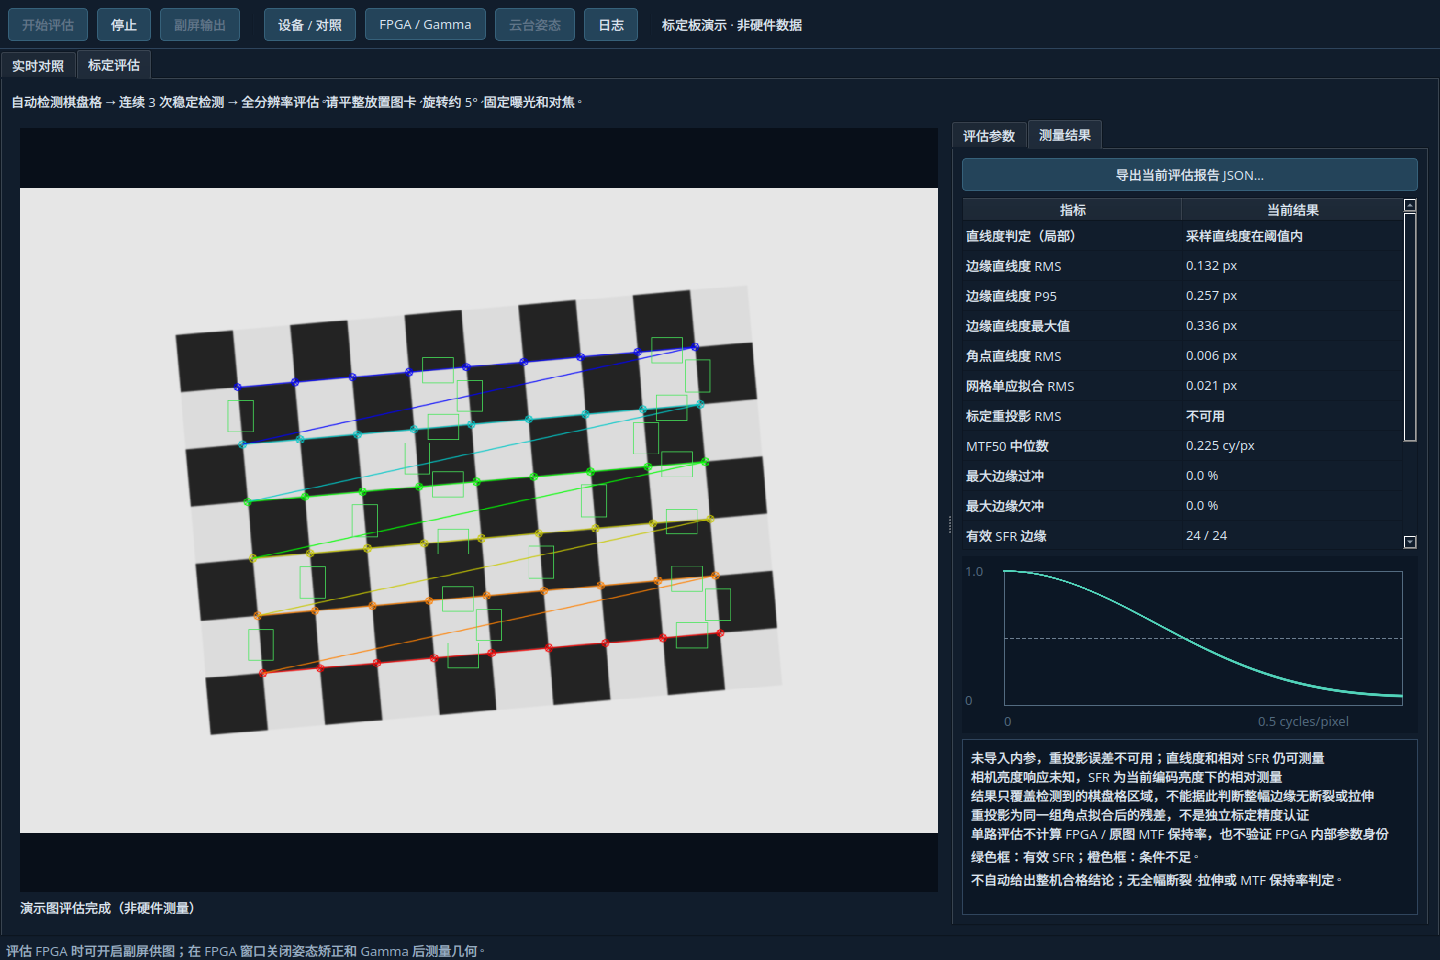
\includegraphics[width=\textwidth]{appendix/appendixC/figures/host_evaluation_demo.png}
\caption{图卡评估界面（工程合成棋盘格演示；图内数值不作为相机或 FPGA 实测结果）}
\label{fig:app-host-evaluation}
\end{figure}

局部直线度默认参考阈值为 RMS 不超过 0.30 px、P95 不超过 0.50 px，
有效边缘采样率至少 80\% 才给出局部阈值判断。
这些值是软件可调整的初始设置，正式验收应采用第~\ref{chap:performance}~章
事先确定的门限，不将默认值写成赛题官方标准。
当前实现不是经过认证的 ISO 12233 测量工具，
也不自动评估整幅拉伸、断裂或给出整机合格结论。

\subsection{标定参数与 JSON 报告}
标定解析器支持附录~\ref{app:camera-calibration}~的 MATLAB JSON，
也支持 OpenCV Brown 模型的 JSON 和 YAML 文件。
MATLAB 内参先转置，再按显式像素起点将主点减 1；
不支持的鱼眼、非零 skew 等模型应拒绝，
图像尺寸不符时不自动缩放内参。
已矫正图像使用实际输出内参和零畸变系数进行参考重投影，
原始图像才允许额外的软件去畸变，避免重复处理。

导入参数只用于 PC 分析，不下发 FPGA，也不能证明硬件内部参数一致。
输出 JSON 保留图像尺寸、图卡、输入几何、软件参考开关、
参数路径与 SHA256、实际 K/D、逐边 ROI 与 SFR、无效原因、阈值和输入接收信息。
对采集卡可附带分析前查询到的功能状态，
但串口状态与视频没有硬件逐帧同步，当前也不计算同步原图/FPGA 图的 MTF 保持率。

导出操作应在停止或切换页面之前进行；
目前 JSON 不包含原始图像，需另外保存原图、曝光/格式、图卡位置和 FPGA 位流信息，
才能按第七章方案复核测量条件。
\sourcefile{\path{../PC/fpga_host/evaluation/}；
\path{../PC/fpga_host/devices/evaluation.py}；
\path{../PC/docs/evaluation.md}}

\section{部署、联调与软件验证}
\subsection{启动与实物操作流程}
在 PC 工程目录建立 Python 虚拟环境并安装 \path{requirements.txt}，
依赖为 PySide6-Essentials、NumPy、opencv-python-headless 和 pyserial。
Linux 硬件模式建议准备 FFmpeg、v4l2-ctl 和 xrandr，
采用 headless OpenCV 可避免其 Qt 插件与 PySide6 冲突。
常用启动命令为
\begin{quote}\small\ttfamily
python -m fpga\_host --demo\\
python -m fpga\_host --config ./settings.json
\end{quote}
首条命令用于无设备界面演示，第二条使用指定配置运行硬件模式。
配置按版本和字段类型校验，并以临时文件替换方式保存；
设备或模型设置应在停止后修改。

\begin{enumerate}
\item 核对 USB 相机、HDMI 采集卡、CP210x 与 STM32 CDC 为正确且不同的设备节点，
下载支持当前协议的 FPGA 位流并启动 STM32 固件。
\item 在系统中启用独立扩展副屏，确认物理信号为 $1920\times1080$、约 60 Hz，
再选定副屏名称；避免镜像、桌面缩放或远程桌面改变输出条件。
\item 连接设备，分别检查两路实际采集与预览 fps，打开副屏输出向 FPGA 供图。
\item 查询 FPGA 状态，提交功能掩码，等待 pending 清除，
再观察输出变化；无输入 SOF 时保留等待提示。
\item 转动 IMU 检查三轴正负号，用模型方向和零点设置辅助观察，
同时按附录~\ref{app:attitude-estimation}~核对实际相机坐标。
\item 定量评估时固定图卡、对焦、曝光与格式，关闭姿态矫正及 Gamma，
采用明确的去畸变开关和输入几何设置，保存全分辨率图像与 JSON。
\end{enumerate}

\subsection{本次软件测试结果}
2026 年 10 月 25 日，使用 PC 工程已有虚拟环境，在 Qt offscreen 模式执行
\begin{quote}\small\ttfamily
QT\_QPA\_PLATFORM=offscreen \textbackslash{}\\
python -B -m unittest discover -s tests -v
\end{quote}
该命令在 PC 工程根目录运行，反斜杠表示 shell 续行。
本次 51 项测试全部通过，无失败或跳过，耗时约 41.3 s。
测试日志与源码身份记录保存在 \path{appendix/references/}。

\begin{table}[htbp]\centering\small
\caption{本次上位机自动测试结果}\label{tab:app-host-tests}
\begin{tabularx}{\textwidth}{>{\raggedright\arraybackslash}p{3.0cm}cY}
\toprule
测试文件 & 数量 & 主要检查内容（均通过） \\
\midrule
\path{test_protocols.py} & 12 & 协议样例、拆包/粘包、噪声重同步、有符号角度、统计合法性及序号门控 \\
\path{test_core.py} & 7 & 缓冲时间/容量、配置校验、实际 URDF 资源和关节变换、显示模式识别 \\
\path{test_serial.py} & 2 & POSIX 虚拟串口、遥测与 ACK 交错、pending、无响应超时及不重放 SET \\
\path{test_video.py} & 10 & JPEG 分帧、FFmpeg 管道、慢解码跳帧、预览延时与副屏独立、断连失效 \\
\path{test_evaluation.py} & 12 & MATLAB/OpenCV 参数、解析高斯斜边、弯曲网格、重投影及评估取消 \\
\path{test_ui.py} & 8 & Qt 演示交互、双路后台解码、页面互斥、静态输入及 JSON 导出 \\
\bottomrule
\end{tabularx}
\end{table}

以上测试验证软件解析、数值趋势、线程调度及界面行为。
合成高斯斜边和棋盘格通过，不代表真实图卡的 MTF50 或直线度已经达标；
虚拟串口通过，也不能替代实际 USB、双屏物理时序与设备断连测试。
实物联调仍需记录两路采集格式和吞吐、正确的副屏输出、长时间运行、
拔插恢复、实际图卡评估与最终 FPGA 位流身份。
\sourcefile{\path{../PC/tests/}；
\path{appendix/references/pc_unittest_20261025.txt}；
\path{appendix/references/source_manifest_20261025.json}}

\end{document}
